\documentclass[11pt]{formatting-template}

% [ ] add figs & tables
% [ ] add text refs to figs & tables
% [ ] After all text added, replace: single and double quotes, escape ampersands
% BUG OK bibtex no \citation commands 

% mathptmx is a Times Roman look-alike (don't use the times package)
% It isn't clear if Times is required. The OGS manual lists several
% "standard fonts" but never says they need to be used.
% \usepackage{mathptmx}

\usepackage[NoDate]{currvita}
\usepackage{array}
\usepackage{tabularx}
\usepackage{booktabs}
\usepackage{ragged2e}
\usepackage{microtype}
\usepackage[breaklinks=true,pdfborder={0 0 0}]{hyperref}
\usepackage{graphicx}
\AtBeginDocument{%
	\settowidth\cvlabelwidth{\cvlabelfont 0000--0000}
}

% OGS recommends increasing the margins slightly.
\increasemargins{.1in}

\usepackage[english]{babel}
\usepackage{blindtext}

\usepackage{url}

\usepackage[super,sort&compress]{natbib}
% The following package was added to add one bibliography per chapter
\usepackage[sectionbib]{chapterbib}

\overfullrule5pt

% Added for merged rows
\usepackage{multirow}

%%%%%%%%%%%%%%%%%%%%%%%%%%%%%%%%%%%%%%%%%%%%%%%%%%%%%%%%%%%%%%%%%%%%%%%%%%%%%%%%
% Thesis Title & Author Information
\title{Integrating Functional Genomics and Human Genetics to Identify Causal Mechanisms for Insulin Resistance}
\author{Xiaomi Du}
\degree{Bioinformatics \& Systems Biology}{Doctor of Philosophy}

% Thesis Committee Members
\chair{Professor Amit R. Majithia}
\cochair{Professor Christopher Glass} 
\committee{Professor Alejandro Chavez} % alphabetical order required
\committee{Professor Terry Gaasterland}
\committee{Professor Yury Miller}
\degreeyear{2026}

%%%%%%%%%%%%%%%%%%%%%%%%%%%%%%%%%%%%%%%%%%%%%%%%%%%%%%%%%%%%%%%%%%%%%%%%%%%%%%%%
\begin{document}

% Begin with front matter and so forth
\frontmatter
\maketitle{}
\makecopyright{}
\makesignature{}

%%%%%%%%%%%%%%%%%%%%%%%%%%%%%%%%%%%%%%%%%%%%%%%%%%%%%%%%%%%%%%%%%%%%%%%%%%%%%%%%
% Dedication
%%%%%%%%%%%%%%%%%%%%%%%%%%%%%%%%%%%%%%%%%%%%%%%%%%%%%%%%%%%%%%%%%%%%%%%%%%%%%%%%
\begin{dedication}
	\setsinglespacing{}
	\parindent0pt\parskip\baselineskip{}
	\vskip0pt plus.25fil
	\begin{center}
		
		This dissertation is dedicated to my family, friends, and scientific mentors.
		
		Thank you for your support. I could not have done this without you. 
		
	\end{center}
\end{dedication}

%%%%%%%%%%%%%%%%%%%%%%%%%%%%%%%%%%%%%%%%%%%%%%%%%%%%%%%%%%%%%%%%%%%%%%%%%%%%%%%%
% Table of Contents, Figures, Tables, Etc.
%%%%%%%%%%%%%%%%%%%%%%%%%%%%%%%%%%%%%%%%%%%%%%%%%%%%%%%%%%%%%%%%%%%%%%%%%%%%%%%%
% Next comes the table of contents, list of figures, list of tables,
% etc. If you have code listings, you can use \listoflistings (or
% \lstlistoflistings) to have it be produced here as well. Same with
% \listofalgorithms.

\tableofcontents
\listoffigures
\listoftables

%%%%%%%%%%%%%%%%%%%%%%%%%%%%%%%%%%%%%%%%%%%%%%%%%%%%%%%%%%%%%%%%%%%%%%%%%%%%%%%%
% Acknowledgements
%%%%%%%%%%%%%%%%%%%%%%%%%%%%%%%%%%%%%%%%%%%%%%%%%%%%%%%%%%%%%%%%%%%%%%%%%%%%%%%%
\begin{acknowledgements}

\noindent Thank you to everyone who joined me on this journey. 

Chapters 1 and 2, in full, are modified for this thesis from the material in Diabetes 2025. The dissertation/thesis author was the primary investigator and author of this paper. I would like to acknowledge my co-authors for the research in Chapters 1 and 2, Karen Mendez-Lara, Siqi Hu, Rachel Diao, Guru Bhavimani, Ruben Hernandez, Kimberly Glass, Camila De Arruda Saldanha, Jason Flannick, Sven Heinz, and Amit Majithia. Thank you for the years of teamwork, weekly meetings, and too many plates of cells.

I would also like to thank my committee members for all their support. Amit Majithia, for taking me on as a graduate student. Chris Glass, for all the advice from first year to my last. Yury Miller, for patiently answering all my questions about macrophages and lipids. Alex Chavez, for his insight on genetic screens and CRISPRa. Terry Gaasterland, for always pushing me to succeed. There are not enough words to express my gratitude. 

Thank you to my mom and dad, who always believed in me, even when I did not. To my brother, Yulin, for inspiring me every day. To my yeye, who liked problem solving through reading books. To all of my family, for their love and support, even from afar. 

Thank you to my friends for filling this experience with laughter, hope, and great food. To Courtney Chen, for always seeing potential in me. To Grace Park, who never gave up on me. To Michelle Ragsac-Mah, the best landlord I could ever ask for. To my graduate school roommates, Alexa Rodriguez, Vanessa Yu, Dinah Shi, Clarence Mah, and Alex Wenzel. To Nena, Arabella, Chloe, Daisy, and Yuuki, for being the best emotional support. To all my hiking buddies, the Saturday b(run)ch club, the cute bioinfo group, the reality tv crew, and everyone else who brought joy to these years - thank you thank you thank you.

Thank you to UCSD and the BISB community, all the faculty, staff, and students who helped along the way. To Hagit Neta, Rizaldy Zapata, Maryam Jalali, and Alex Blee, for keeping the lab running with your wisdom. To Rachel Diao, Karen Mendez-Lara, Guru Bhavimani, Siqi Hu, and Camila De Arruda Saldanha, for all the shared wet lab guidance and support. To the bioinformatics corner, Natalie DeForest, Emily Kobayashi, and Michelle Wang. To GTP and Bruce Hamilton, for training me to be a better scientist. 

Thank you to Demetrios Braddock, for accepting a high school junior into your lab and teaching me the joy of scientific research. To David Baltimore and Arnav Mehta, for giving me the opportunity to learn and perform cutting edge science. To Ci Chu and Charlie Kim, for inspiring my interest in computational biology and functional genomics. And to Taylor Oniskey, for convincing me to apply for graduate school.	

Thank you, all. 
\end{acknowledgements}

%%%%%%%%%%%%%%%%%%%%%%%%%%%%%%%%%%%%%%%%%%%%%%%%%%%%%%%%%%%%%%%%%%%%%%%%%%%%%%%%
% Vita
%%%%%%%%%%%%%%%%%%%%%%%%%%%%%%%%%%%%%%%%%%%%%%%%%%%%%%%%%%%%%%%%%%%%%%%%%%%%%%%%
\begin{vita}
\noindent
\begin{cv}{}
\begin{cvlist}{}
	\item[2012--2016] B.S. in Biology\\
		California Institute of Technology (Caltech)
	\item[2016--2019] Genomics Research Associate\\
		Verily Life Sciences
	\item[2019--2026] Ph.D. in Bioinformatics \& Systems Biology\\
		University of California San Diego
\end{cvlist}
\end{cv}

%%%%% PUBLICATIONS %%%%%
\publications{}

\noindent Cunha E Rocha K, Tan B, Kempf J, Medina C, Beldona V, Qian C, Duan Y, Xiang Q, Yoo A, \textbf{Du X}, Majithia AR, Ying W. 2025. Adipose tissue macrophage-derived miR-690 modulates adipocyte precursor cell maintenance and adipogenesis. Mol Metab 101:102246.
\\

\noindent \textbf{Du X}, Mendez-Lara K, Hu S, Diao R, Bhavimani G, Hernandez R, Glass K, De Arruda Saldanha C, Flannick J, Heinz S, Majithia AR. 2025. An alternatively translated isoform of PPARG suggests AF-1 domain inhibition as an insulin sensitization target. Diabetes 74:651–663.
\\

\noindent DeForest N, Kavitha B, Hu S, Isaac R, Krohn L, Wang M, \textbf{Du X}, De Arruda Saldanha C, Gylys J, Merli E, Abagyan R, Najmi L, Mohan V, Alnylam Human Genetics, AMP-T2D Consortium, Flannick J, Peloso GM, Gordts PLSM, Heinz S, Deaton AM, Khera AV, Olefsky J, Radha V, Majithia AR. 2023. Human gain-of-function variants in HNF1A confer protection from diabetes but independently increase hepatic secretion of atherogenic lipoproteins. Cell Genom 3:100339.
\\

\noindent Guo MH, Sama P, LaBarre BA, Lokhande H, Balibalos J, Chu C, \textbf{Du X}, Kheradpour P, Kim CC, Oniskey T, Snyder T, Soghoian DZ, Weiner HL, Chitnis T, Patsopoulos NA. 2022. Dissection of multiple sclerosis genetics identifies B and CD4+ T cells as driver cell subsets. Genome Biol 23:127.
\\

\noindent \textbf{Du X}, DeForest N, Majithia AR. 2021. Human genetics to identify therapeutic targets for NAFLD: Challenges and opportunities. Front Endocrinol (Lausanne) 12:777075.
\\

\noindent Mehta A, Mann M, Zhao JL, Marinov GK, Majumdar D, Garcia-Flores Y, \textbf{Du X}, Erikci E, Chowdhury K, Baltimore D. 2015a. The microRNA-212/132 cluster regulates B cell development by targeting Sox4. J Exp Med 212:1679–1692.
\\

\noindent Mehta A, Zhao JL, Sinha N, Marinov GK, Mann M, Kowalczyk MS, Galimidi RP, \textbf{Du X}, Erikci E, Regev A, Chowdhury K, Baltimore D. 2015b. The MicroRNA-132 and MicroRNA-212 cluster regulates hematopoietic stem cell maintenance and survival with age by buffering FOXO3 expression. Immunity 42:1021–1032.

%%%%% FIELDS OF STUDY %%%%% 
% This section was omitted within this thesis as it was optional.

\end{vita}

%%%%%%%%%%%%%%%%%%%%%%%%%%%%%%%%%%%%%%%%%%%%%%%%%%%%%%%%%%%%%%%%%%%%%%%%%%%%%%%%
% Dissertation Abstract 
%%%%%%%%%%%%%%%%%%%%%%%%%%%%%%%%%%%%%%%%%%%%%%%%%%%%%%%%%%%%%%%%%%%%%%%%%%%%%%%%
\begin{dissertationabstract}
Insulin resistance, defined by decreased sensitivity in target tissues to normal circulating levels of insulin, underlies the pathogenesis of many epidemic metabolic disorders, including type 2 diabetes, metabolic syndrome, and cardiovascular disease. In this dissertation, I leverage functional genomics and human genetics to further our understanding of the molecular mechanisms driving insulin resistance, with a particular focus on peroxisome proliferator–activated receptor $\gamma$ (PPAR$\gamma$), the pharmacologic target of thiazolidinediones, a class of potent insulin sensitizers limited by adverse effects, and adipose tissue biology. In Chapter 1, I apply high-throughput genome engineering to systematically perturb PPARG, revealing an alternative translational start site that generates a truncated isoform, PPAR$\gamma$ M135, with increased transactivation in response to thiazolidinediones. In Chapter 2, I investigate the metabolic consequences of PPAR$\gamma$ M135 using a human preadipocyte cell line model and through genetic analysis of rare variants that recapitulate the functional effects of this isoform, highlighting its insulin sensitizing potential. Adipose tissue plays a central role in systemic insulin sensitivity, with distinct fat depots contributing differently to metabolic health: while subcutaneous adipose tissue is considered protective, visceral adipose tissue is associated with insulin resistance and cardiometabolic disease. However, mechanistic studies of depot-specific functions have been limited by the lack of human visceral adipocyte cell lines. To address this, in Chapter 3, I describe a framework for reprogramming an existing cell model into depot-specific adipocytes to provide more resources for future studies of insulin resistance. Altogether, in this dissertation, I combine functional genomics with human genetics to identify an alternatively translated isoform with insulin sensitizing implications and establish the foundation for more depot-specific analysis of insulin resistance in adipocytes.
\end{dissertationabstract}

%%%%%%%%%%%%%%%%%%%%%%%%%%%%%%%%%%%%%%%%%%%%%%%%%%%%%%%%%%%%%%%%%%%%%%%%%%%%%%%%
% Main Text of the Dissertation
%%%%%%%%%%%%%%%%%%%%%%%%%%%%%%%%%%%%%%%%%%%%%%%%%%%%%%%%%%%%%%%%%%%%%%%%%%%%%%%%
\mainmatter{}

\begin{dissertationintroduction}
    
\setcounter{chapter}{0}
\chapter*{Introduction}

\label{chap:introduction}

Insulin resistance (IR) is a condition of decreased sensitivity to normal circulating levels of insulin in target tissues. It is the root cause of many epidemic diseases and conditions, including type 2 diabetes (T2D), cardiovascular disease (CVD), and metabolic syndrome (MetS)\cite{James2021-vu,Adeva-Andany2019-df,Park2024-da}. In addition to its clinical heterogeneity, there are also many insulin responsive tissues, including the liver, adipose tissue, and skeletal muscle, and many cell types that facilitate crosstalk between the different organs. Changes in one tissue or cell type can perturb whole body IR\cite{James2021-vu}.  

One class of drugs directly reduces IR by increasing insulin sensitivity. Thiazolidinediones (TZDs) decrease IR by agonizing PPAR$\gamma$\cite{Yki-Jarvinen2004-bc}, a nuclear hormone receptor encoded by gene \textit{PPARG}. TZDs have demonstrated clinical efficacy in treating T2D, CVD, and metabolic dysfunction-associated steatotic liver disease (MASLD), but their use has been limited by serious side effects, such as weight gain and fluid retention, which are a direct consequence of PPAR$\gamma$ agonism through interaction at its ligand-binding domain (LBD)\cite{Kernan2016-as,Musso2017-xi,Arnold2019-kq}. Much pharmacological development has been focused on the development of selective PPAR$\gamma$ modulators that retain the benefits of TZDs without the attendant adverse effects, but successful compounds have not reached the clinic\cite{DePaoli2014-lp,Higgins2010-yv}. Thus, the need for alternative approaches to therapeutically activate PPAR$\gamma$ without PPAR-mediated side effects remains unmet.  

Intriguingly, TZDs lead to weight gain by increasing a specific depot of adipose tissue that is metabolically beneficial\cite{Zhang2024-sl}. Previously, adipose tissue was regarded as only an energy reservoir, and it was understudied compared to other organs \cite{Sebo2019-nh}. We now know it is a dynamic endocrine organ that plays a central role in many physiological processes, including insulin sensitivity and immune responses\cite{Sakers2022-wb}. It is found throughout the human body, with tissue and organ specific depots, but white adipose tissue is generally categorized as either subcutaneous fat, located beneath the skin, or visceral fat, which surrounds the internal organs. Subcutaneous adipose tissue (SAT) is considered metabolically beneficial, while visceral adipose tissue (VAT) is unfavorable\cite{Mathur2022-fx}. Increased VAT is associated with higher risk of both T2D and CVD, whereas SAT is neutral or even protective\cite{Agrawal2023-ee}. While there have been many investigations on differential gene expression and cytokine secretion between SAT and VAT\cite{Mathur2022-fx,Ahn2019-us,Passaro2017-zk,Gesta2006-so,Tchkonia2007-xa,Wajchenberg2002-pt,Lee2010-fl}, the molecular basis of SAT and VAT heterogeneity is largely unknown. Further study of the mechanistic differences between adipocytes in SAT and VAT could elucidate how they contribute to metabolic health in opposing manners.   

While there are lifestyle factors that contribute to metabolic health, genetics also play a role in determining risk of IR and its associated diseases\cite{James2021-vu}. Genome-wide association studies (GWAS) have identified many loci associated with MetS\cite{Park2024-da}, but most GWAS do not include rare variants, which have a larger effect size\cite{Wang2021-au}. Moreover, after identification, the causal genes, mechanisms of action, and tissues of effect need to be elucidated for GWAS loci. Functional genomics studies how genotype affects phenotype at the genome-wide scale through the analysis of genes, RNA transcripts, proteins, and other biological components\cite{Farrell2017-lq}. Genome editing is a common method applied in functional genomics to both isolate causal variants from GWAS loci and enable characterization of the causal genes. The recent development of single cell CRISPR methods, such as Perturb-seq and CROP-seq, produce higher resolution cell phenotypes, generating whole transcriptomes of edited cells\cite{Datlinger2017-yc,Dixit2016-yg}. Combined with the hypotheses generated from GWAS, large screens, and cell atlases, single cell CRISPR and other functional genomics methods can help determine mechanisms underlying IR.   

In this dissertation, I present the following three chapters in which I leverage functional genomics and human genetics to study the role of \textit{PPARG} in insulin resistance and establish the framework to compare matched subcutaneous and visceral adipocytes in vitro.  

In Chapter 1, I perform a genome editing screen across \textit{PPARG} to investigate the effects of edits on each coding exon of the gene. This screen was performed with CRISPR-Cas9 in a human monocyte cell line, THP-1, which is a suitable model for large scale genetic perturbation that phenocopies \textit{PPARG} related transcriptional responses in adipocytes\cite{Majithia2016-bm,Agostini2018-bx}. We discovered that edits in the 5’ end of the gene still generated a functional isoform of PPAR$\gamma$, indicative of an alternative translational start site. These results were corroborated with analysis of an analogous screen that introduced the edited PPARG transcripts exogenously, and the findings were characterized with gene and protein expression. A truncated isoform, referred to as PPAR$\gamma$ M135, can be translated from methionine encoded by codon 135, and this isoform has higher transactivation of canonical PPAR$\gamma$ target genes in response to TZDs.  

In Chapter 2, I extend the findings of Chapter 1 to study the insulin sensitizing capacity of the novel PPAR$\gamma$ isoform. We generated adipocytes that express PPAR$\gamma$ M135 and found significantly increased insulin sensitizing activity in cells with PPAR$\gamma$ M135 as opposed to the endogenous PPAR$\gamma$2 isoform. Additionally, human carriers of rare variants in PPARG were evaluated for the severity of metabolic syndrome and insulin resistance, as measured by the triglyceride to HDL (TG/HDL) ratio. Human carriers of variants with decreased function in the N-terminal portion of PPAR$\gamma$, upstream of p.M135, have nominally lower metabolic syndrome severity and insulin resistance than carriers of variants with decreased function downstream of p.M135. Altogether, the data suggests that PPAR$\gamma$ M135 can be metabolically beneficial in humans as a result of increased insulin sensitization.   

In Chapter 3, I present the analytical framework of how to reprogram preadipocytes into depot-specific adipocytes. I identify factors to reprogram cells into either subcutaneous or visceral adipocytes using established methods and evaluate them on independent transcriptomic datasets. I further detail how to evaluate reprogrammed cells using pseudobulks of single cell/nuclei RNA-sequencing.   

In summary, my dissertation applies functional genomics to investigate genes and tissues that contribute to insulin resistance. Through genetic screens, transcriptomics, and proteomic analysis, I uncovered an alternative translational start site in PPARG that generates PPAR$\gamma$ M135, an isoform with increased transactivation in response to TZDs. PPAR$\gamma$ M135 results in increased insulin sensitivity, as measured in an adipocyte cell line and supported by analysis of human carriers. I additionally propose detailed methods for reprogramming and evaluating depot-specific adipocytes to deepen our understanding of adipocytes and enable further research into their function. In total, my dissertation aims to extend research on genes and cell types critical to preventing insulin resistance.

\end{dissertationintroduction}

\bibliographystyle{unsrtnat}
\bibliography{bib_0.bib}

% \chapter{An alternative translational start \texorpdfstring{site \\identified}{site identified} in \texorpdfstring{\(PPARG\)}{PPARG} generates \texorpdfstring{a \\functional}{a functional} isoform
\chapter{An alternative translational start site identified in PPARG generates a functional isoform
}\label{chap:chapter 1}

%%%%%%%%%%%%%%%%%%%%%%%%%%%%%%%%%%%%%%%%%%%%%%%%%%%%%%%%%%%%%%%%%%%%%%%%%%%%%%%%
\section{Introduction}
%%%%%%%%%%%%%%%%%%%%%%%%%%%%%%%%%%%%%%%%%%%%%%%%%%%%%%%%%%%%%%%%%%%%%%%%%%%%%%%%

Insulin resistance is a major driver of the epidemic diseases, type 2 diabetes, cardiovascular disease (CVD), and nonalcoholic fatty liver disease (NAFLD), that challenge global health\cite{James2021-vu,Adeva-Andany2019-df,Khan2019-qt}. Thiazolidinediones (TZDs) are a class of drugs that decrease insulin resistance by agonizing PPAR$\gamma$\cite{Yki-Jarvinen2004-ba}, a nuclear hormone receptor that contains an autonomous activation-function domain 1 (AF-1), DNA binding domain (DBD), and ligand binding domain (LBD) (\textbf{Figure 1.1A})\cite{Tontonoz1994-nk}. TZDs have demonstrated clinical efficacy in treating type 2 diabetes, CVD, and NAFLD\cite{Kernan2016-fd,Inzucchi2016-ni,Musso2017-xi}, but their use has been limited by serious side effects, such as weight gain and fluid retention, which are a direct consequence of PPAR$\gamma$ agonism through interaction at its ligand-binding domain (LBD)\cite{Yki-Jarvinen2004-ba}. Much pharmacological development has been focused on the development of selective PPAR$\gamma$ modulators (SPPARMs) that retain the benefits of TZDs without the attendant adverse effects, but successful compounds have not reached the clinic\cite{Higgins2010-tv,DePaoli2014-hi}. Thus, the need for alternative approaches to therapeutically activate PPAR$\gamma$ without PPAR-mediated side effects remains unmet.

In this study, we report a novel protein isoform of PPAR$\gamma$ (named PPAR$\gamma$ M135), which lacks the AF-1 domain and is generated from an alternative translational start site (hg38:chr3:12381414). Through biochemical and transcriptomic profiling, we find that PPAR$\gamma$ M135 demonstrates enhanced ligand-inducible transcriptional and functional activity compared to wild-type (WT), leading us to a model of de-repression by loss of AF-1.

%%%%%%%%%%%%%%%%%%%%%%%%%%%%%%%%%%%%%%%%%%%%%%%%%%%%%%%%%%%%%%%%%%%%%%%%%%%%%%%%
\section{Results}
%%%%%%%%%%%%%%%%%%%%%%%%%%%%%%%%%%%%%%%%%%%%%%%%%%%%%%%%%%%%%%%%%%%%%%%%%%%%%%%%

\subsection{A novel functional PPAR\texorpdfstring{$\gamma$}{gamma} isoform, M135, is generated from an alternative translational start site}

In our initial experiments the endogenous \(PPARG\) locus was systematically disrupted by inducing insertions and deletions (indels) in each coding \(PPARG\) exon in a human macrophage cell line (THP-1), a tractable model suitable for large scale genetic perturbation that we and others have shown phenocopy \(PPARG\) related transcriptional responses in adipocytes\cite{Majithia2016-bm,Agostini2018-bx}. Findings from THP-1s were confirmed and extended in human adipocytes models, the physiologically relevant cell type for metabolic disease. The effect of \(PPARG\) disruptions was measured by quantifying the ability of the resulting cells to transactivate CD36, a direct PPAR$\gamma$ transcriptional target\cite{Tontonoz1998-aq}. A custom lentiviral library of CRISPR/Cas9 constructs with guides (sgRNAs) targeting all coding exons, untranslated regions, and introns (n=95), was introduced into THP-1 monocytes at one construct per cell. The resulting population of genome-edited cells was differentiated into macrophages, stimulated with 1 $\mu$M PPAR$\gamma$ agonist rosiglitazone, and sorted by FACS according to the expression of CD36 (\textbf{Figure 1.1B}). The CD36+ and CD36- populations were sequenced to recover the identities of the sgRNAs, and an enrichment score (ES) was calculated based on the counts of each sgRNA in the CD36+/CD36- pools (\textbf{Figure 1.1B, C}). Intron targeting sgRNAs introduced as controls had an average ES of 0.487. As expected, targeting sgRNAs to Exon B of \(PPARG\) (specific to the PPAR$\gamma$2 isoform) did not reduce CD36 activity ($\overline{ES}$=0.622), and most sgRNAs targeted to exons downstream of the PPAR$\gamma$1 start site caused severe loss of CD36 transactivation ($\overline{ES}$=-1.33). Intriguingly, five sgRNAs targeting Exon 1 of \(PPARG\), downstream of the PPAR$\gamma$1 start site, which would be predicted to maximally disrupt the protein sequence, had little effect on CD36 transactivation ($\overline{ES}$=0.629), suggesting an intact PPAR$\gamma$ response in the cells that harbored them (\textbf{Figure 1.1C}).  

\clearpage
\begin{figure}[!t]
    \centering
    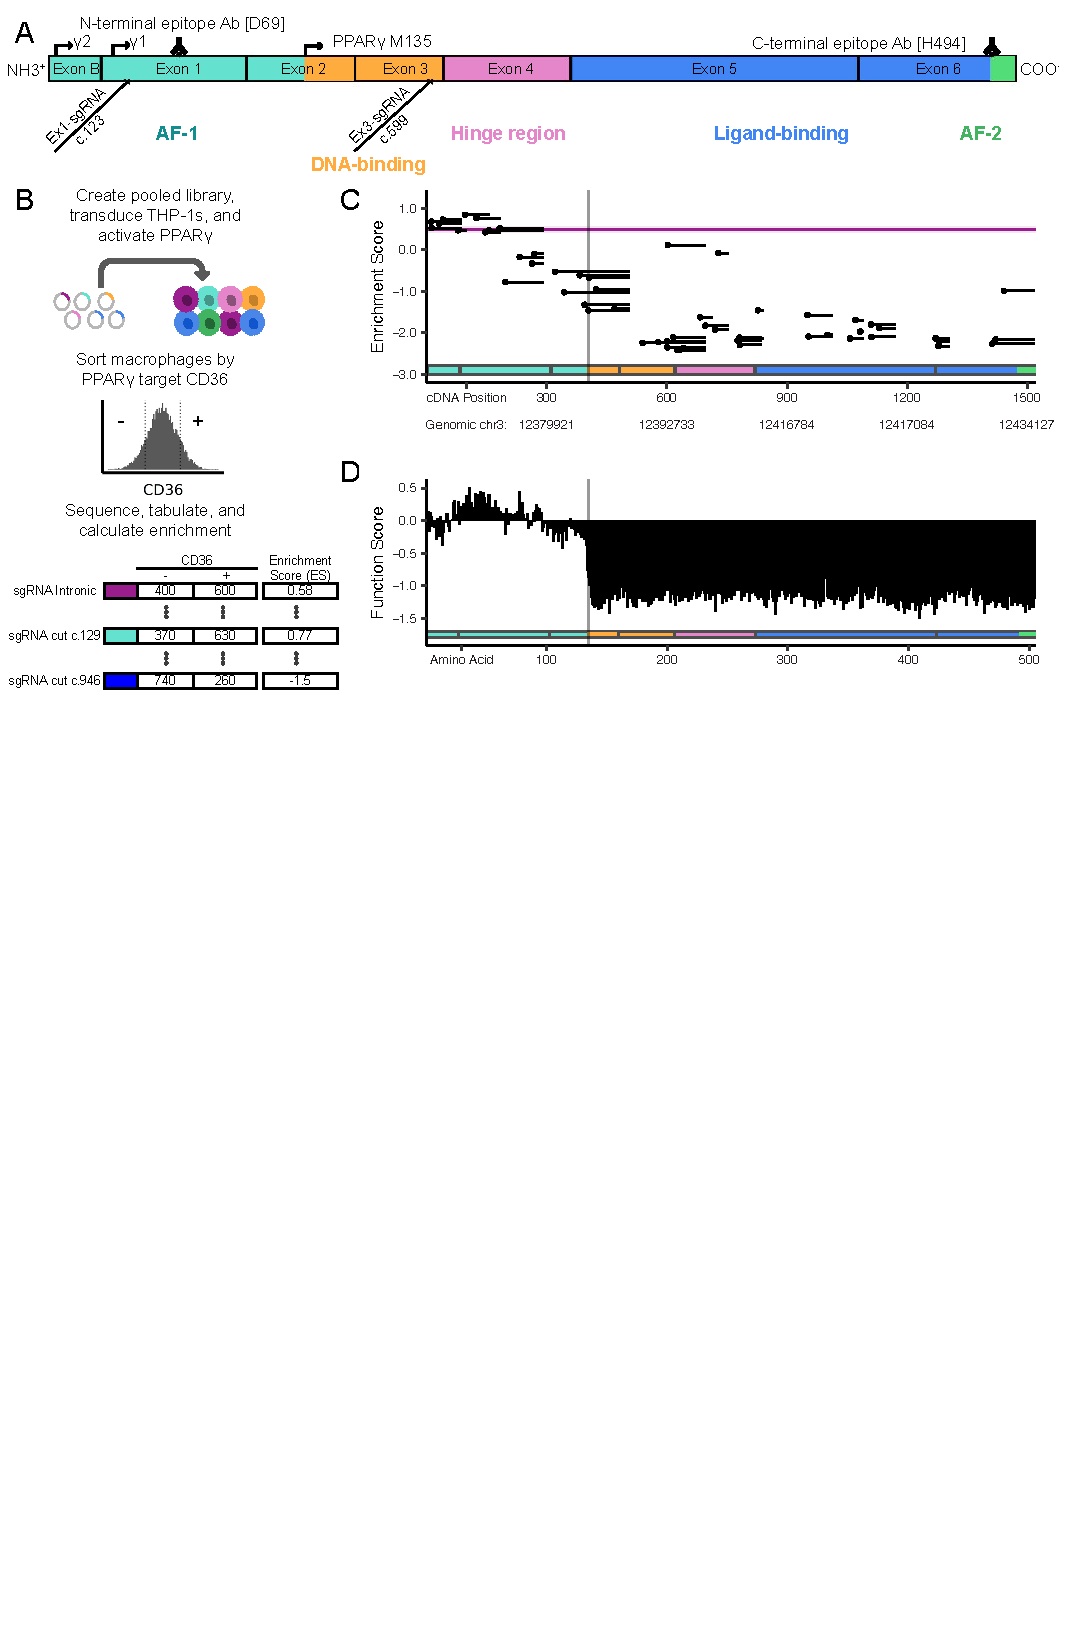
\includegraphics[width=\textwidth]{1_figures-and-files/Fig1.pdf}
    \caption[Functional screens across \(PPARG\) reveal an alternative translational start site at p.M135.]{\textbf{Functional screens across \(PPARG\) reveal an alternative translational start site at p.M135.} A. Linear representation of PPAR$\gamma$ indicating start sites for $\gamma$1, $\gamma$2 and novel M135. Guides and cut sites (Ex1-sgRNA; chr3:12379745 and Ex3-sgRNA; chr3:12392733. hg38) of CRISPR/Cas9 monoclonal generated cells are shown. Domain structure of PPAR$\gamma$ protein is represented in colors, and epitopes of the N-terminus and C-terminus antibodies (Abs) are indicated.  B. A library of 95 guide RNAs (sgRNAs) targeting \(PPARG\) was generated and transduced into THP-1 monocytes, such that each cell received a single construct. The polyclonal THP-1s were differentiated into macrophages, stimulated with a PPAR$\gamma$ agonist, 1 uM rosiglitazone (rosi), and sorted by FACS for expression of PPAR$\gamma$ target CD36 into bins of low (-) and high (+) PPAR$\gamma$ activity (n=5 independent replicate sorts). C. Enrichment scores (ES) from the CRISPR screen across PPARG. The mean ES for each guide across the 5 sort replicates is plotted along the PPARG2 cDNA based on its cut site (dot) and predicted termination after a 1 base indel (line). The horizontal purple line is the mean and standard error (se) of the intronic guides (n=18). PPAR$\gamma$ p.M135 is denoted by the vertical line. D. Function scores (FS) of insertions/deletions (indels) at each amino acid of PPAR$\gamma$2 calculated as previously published (Majithia et al. 2016). FS=0 refers to wild-type activity.
    }\label{fig:1 Alternative translational start site identification}
\end{figure}

To further understand this unexpected finding, we analyzed data generated from a previously conducted saturation mutagenesis study of \(PPARG\) that contained indels at every codon of the PPAR$\gamma$2 cDNA (CCDS2609; \textbf{Figure 1.1D})\cite{Majithia2016-bm}. Most indels that caused frameshift terminations in \(PPARG\) resulted in complete abrogation of rosiglitazone-induced CD36 transactivation, as evidenced by negative function scores (FS, Figure 1.1D). However, frameshifting indels in the 5$^{\prime}$ region of the cDNA, which would be predicted to cause very early termination of protein translation through nonsense disruption of the open reading frame, paradoxically retained cellular PPAR$\gamma$ transactivation ($\overline{FS}$=0.0322). This concurred with our finding of tolerated Exon 1 disruptions at the endogenous \(PPARG\) locus (Figure 1.1C) and suggested a possible post-splicing mechanism for retained PPAR$\gamma$ activity. The tolerance to early frameshifting indels was observed until c.A403 (CCDS2609), after which frameshifting indels showed severe loss of function ($\overline{FS}$=-1.16). These findings were consistent when experiments were performed with prostaglandin J2, a putatively endogenous ligand\cite{Majithia2016-bm} (\textbf{Figure A.1}). The codon at c.A403-405 encodes a methionine, leading us to hypothesize an alternative translation initiation site, which would explain the preservation of PPAR$\gamma$ transactivation functions in transcripts with frameshift and nonsense-inducing indels prior to c.A403.

A translation initiation site at CCDS2609 c.A403 (hg38:chr3:12381414; ENSP00000287820 p.M135) would lead to a protein isoform (PPAR$\gamma$ M135) shorter than PPAR$\gamma$2 by 134 amino acids with a predicted molecular weight of $\sim$40 kDa. To evaluate this hypothesis, we engineered clonal THP-1 monocytes with disruptions in Exon 1, Exon 3, and an intron of PPAR$\gamma$ using CRISPR/Cas9 targeting constructs (Ex1-sgRNA chr3:12379745, Ex3-sgRNA chr3:12392733, Int-sgRNA chr3:12363492, \textbf{Figure 1.1A}). Two independent cell lines were derived for each of the following genotypes: Int-sgRNA +/+, Ex1-sgRNA +/-, Ex1-sgRNA -/-, and Ex3-sgRNA -/- (\textbf{Table A.1}). Following differentiation into macrophages, western blotting was performed using PPAR$\gamma$ antibodies raised against an N-terminal epitope (p.Asp69) and a C-terminal epitope (p.His494). On the N-terminal blot, a 53 kDA band corresponding to full-length PPAR$\gamma$1 can be observed in the control samples (Int-sgRNA) and in the heterozygous Ex1-sgRNA samples, as expected, and no PPAR$\gamma$ bands were detected in the homozygous Ex1-sgRNA or Ex3-sgRNA edited cells (\textbf{Figure 1.2A}). For the Ex1-sgRNA edited cells, the lack of detection on the N-terminal PPAR$\gamma$ blot is consistent with PPAR$\gamma$ M135 lacking the AF-1 domain. The C-terminal PPAR$\gamma$ blot corroborated the detection of full-length PPAR$\gamma$1 and also revealed a series of lower molecular weight bands in the Ex1-sgRNA cell lines, including a band at $\sim$40 kDa that matches the predicted size of PPAR$\gamma$ M135 (\textbf{Figure 1.2B}).

\clearpage
\begin{figure}[h]
    \centering
    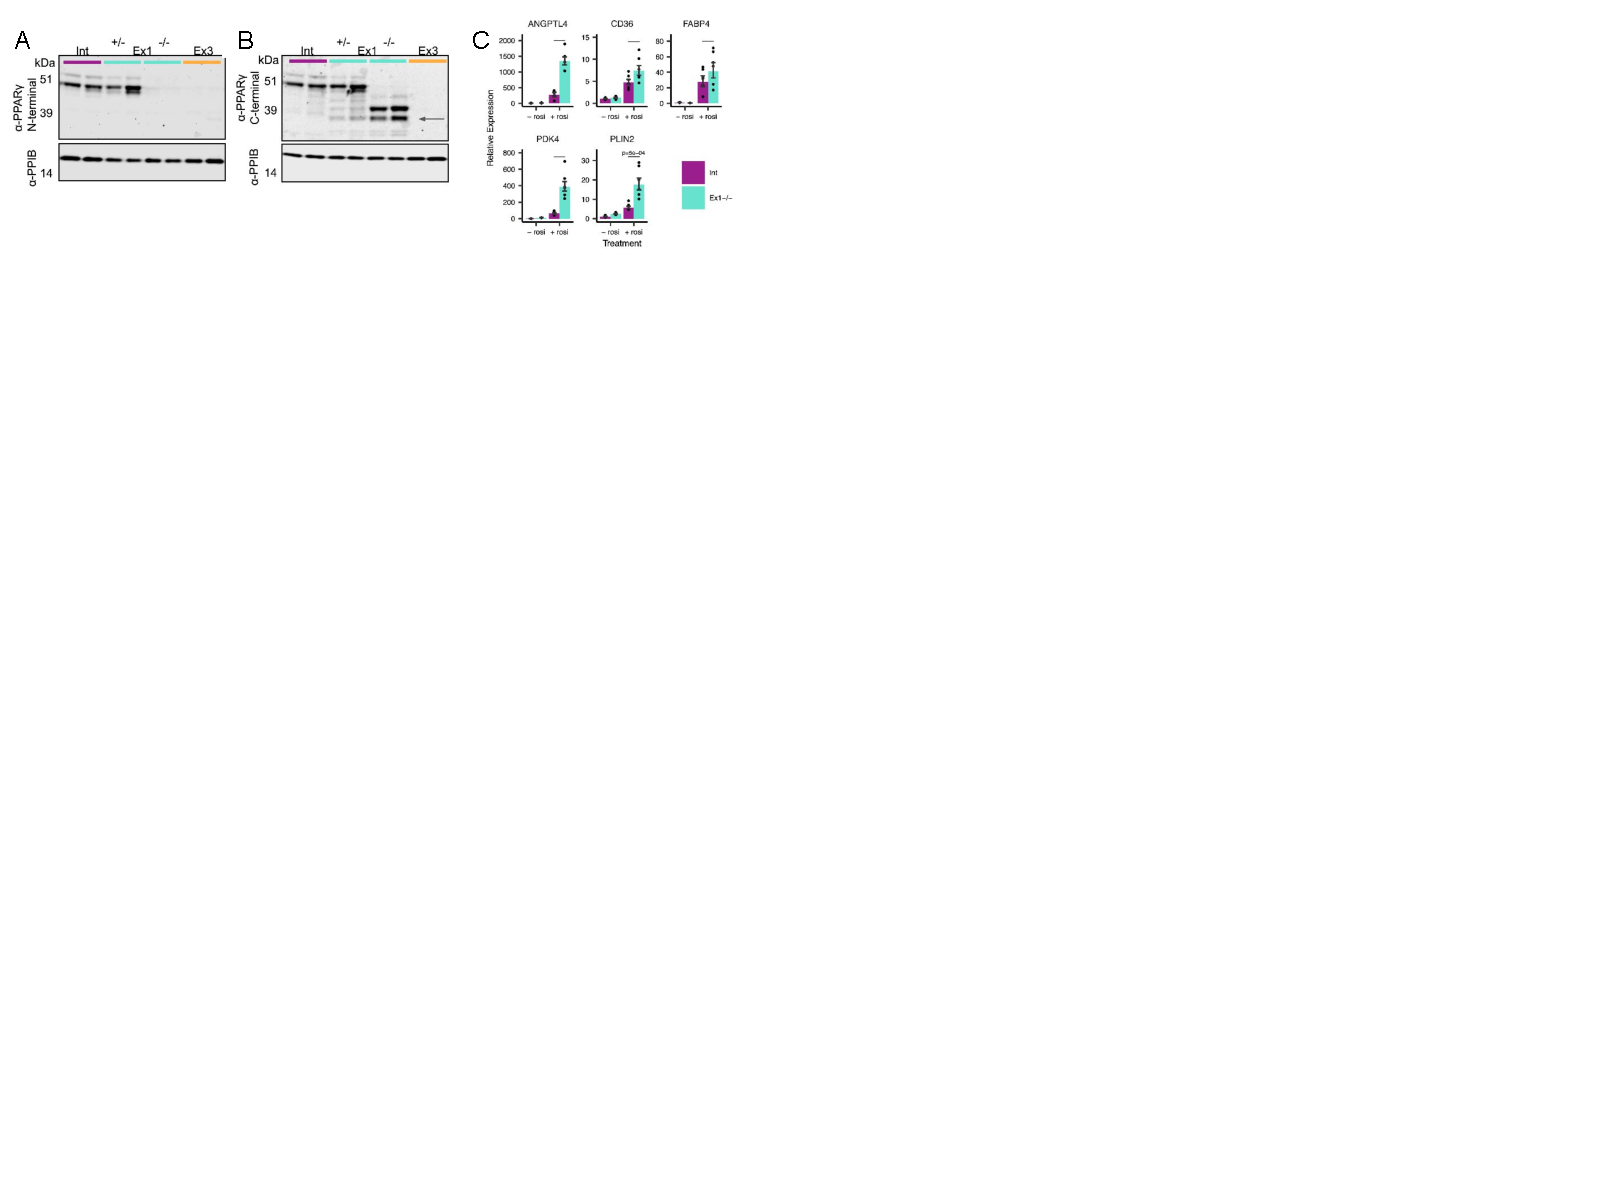
\includegraphics[width=\textwidth]{1_figures-and-files/Fig2.pdf}
    \caption[THP-1 macrophages express a novel isoform of PPAR$\gamma$, named PPAR$\gamma$ M135, when edited upstream of the alternative translational start site.]{\textbf{THP-1 macrophages express a novel isoform of PPAR$\gamma$, named PPAR$\gamma$ M135, when edited upstream of the alternative translational start site.} A. Western blots against the N-terminus and B. C-terminus of PPAR$\gamma$ protein were performed to detect PPAR$\gamma$ isoforms from monoclonal cell lines, evidencing that pre-M135 edited cell lines (Ex1) generate truncated PPAR$\gamma$ bands, including the predicted p.M135 at 40 kDa (arrow) as opposed to post-M135 (Ex3) targeted cell lines and intronic cell lines (Int). C. Relative expression of PPAR$\gamma$ target genes in PPARG targeted monoclonal cell lines, with and without rosiglitazone treatment, with GAPDH as the housekeeping gene and Int-sgRNA edited cells with 0 rosi as control. In response to rosiglitazone, the increases in ANGPTL4, PDK4, and PLIN2 for Ex1 edited cells (n=6, cyan) were greater than the increases in the Int edited cells (n=6, purple) (Welch’s two-sample t-test on delta Ct values). Non-significant increases in CD36 and FABP4 were also observed in Ex1 edited cells.
    }\label{fig:2 THP-1 macrophages can generate novel isoform}
\end{figure}

This 40 kDa band, which was only detected by the C-terminal antibody, had increased intensity in the Ex1-homozygous versus the Ex1-heterozygous cell lines. Some of the other bands detected by the C-terminal antibody could be consistent with translation initiation at AUG codons downstream of the canonical start codon but upstream of p.M135 (e.g. p.M53). Finally, neither the N- or the C-terminal specific antibodies detected protein in the Ex3-sgRNA edited cells, indicating a complete absence of PPAR$\gamma$ protein when Exon 3 is disrupted (\textbf{Figure 1.2B}).

To compare the transcriptional profiles of cells expressing WT and PPAR$\gamma$ M135, the Int-sgRNA +/+ and Ex1-sgRNA -/- clonal cell lines were differentiated into macrophages, stimulated with 1 $\mu$M rosiglitazone and assessed for gene expression at several canonical PPAR$\gamma$ target genes (\textbf{Figure 1.2C}). Upon agonist induction, the Ex1-sgRNA -/- cells expressed significantly higher levels of \(ANGPTL4\)\cite{Aryal2016-ze} (p=0.001), \(PDK4\)\cite{Lefterova2008-rk} (p=6.2e-6), and \(PLIN2\)\cite{Hodgkinson2003-fo} (p=5e-4) than the Int-sgRNA +/+ cells. These PPAR$\gamma$ M135 expressing cells also showed non-significant increases in \(CD36\) and \(FABP4\) expression.

We subsequently isolated and compared the transactivation potentials of WT and PPAR$\gamma$ M135. A PPRE-driven luciferase reporter\cite{Kim1998-aj} and WT PPAR$\gamma$ or PPAR$\gamma$ M135 mRNA were transfected into HEK293s, which have minimal endogenous PPARG activity\cite{Ma2012-dm}. In this system, PPAR$\gamma$ M135 activated transcriptional activity more potently than WT when induced with rosiglitazone (\textbf{Figure A.2a}). We further compared the stability of PPAR$\gamma$ M135 to WT by performing a cycloheximide chase\cite{Hsu1996-yv} in the heterozygous Ex1-sgRNA cells that generate both isoforms (\textbf{Figure A.2b}). The M135 isoform degraded more slowly than PPAR$\gamma$1 (\textbf{Figure A.2c}) which could contribute to its enhanced transactivation potential.

\subsection{Ligand-activated PPAR\texorpdfstring{$\gamma$}{gamma} M135 transactivates target genes more potently than WT PPAR\texorpdfstring{$\gamma$}{gamma} in THP-1s}

We next sought to isolate the activity of PPAR$\gamma$ M135 and evaluate its effect on global transcriptional profiles in comparison with full-length wild-type (WT) PPAR$\gamma$. To compare the direct transcriptional responses of M135 and WT, we performed RNA-seq on PPAR$\gamma$ null (P$\gamma$-/-) THP-1 monocytes electroporated with in vitro transcribed mRNA of each of the two PPAR$\gamma$ isoforms; eGFP mRNA was also electroporated as a process control. In preliminary experiments, mRNA amounts for each isoform were titrated to express similar amounts of protein at the point of harvest (\textbf{Figure A.3}), such that 2 $\mu$g PPAR$\gamma$ M135 mRNA and 8 $\mu$g PPAR$\gamma$ WT were used for each electroporation. The electroporated cells were differentiated into macrophages to mimic the cellular context in which PPAR$\gamma$ is active\cite{Rovera1979-za} and treated with 0 (-) and 1 $\mu$M (+) rosiglitazone. As a positive control, wild-type (P$\gamma$+/+) THP-1 cells with intact \(PPARG\) were also treated with +/- rosiglitazone and transcriptionally profiled (\textbf{Figure 1.3A}).

After filtering for low expression, 16,732 transcripts were retained for analysis across all samples. As expected, rosiglitazone treatment increased gene expression of canonical PPAR$\gamma$ target genes including \(CD36\), \(FABP4\)\cite{Tontonoz1994-nk}, and \(PLIN2\)\cite{Hodgkinson2003-fo} (\textbf{Figure 1.3B}). Remarkably, PPAR$\gamma$ M135-electroporated (P$\gamma$-/- +M135) cells exhibited greater agonist-induced transcriptional responses for some of these targets compared to P$\gamma$-/- +WT or P$\gamma$+/+ THP-1 macrophages, despite comparable PPAR$\gamma$ protein levels (log2 fold-change (log2FC): \(CD36\): P$\gamma$-/- +M135=4.22, P$\gamma$+/+ =2.94, P$\gamma$-/- +WT=1.62. \(PLIN2\): P$\gamma$-/- +M135=3.35, P$\gamma$+/+=3.24, P$\gamma$-/- +WT=1.50).

\clearpage
\begin{figure}[!t]
    \centering
    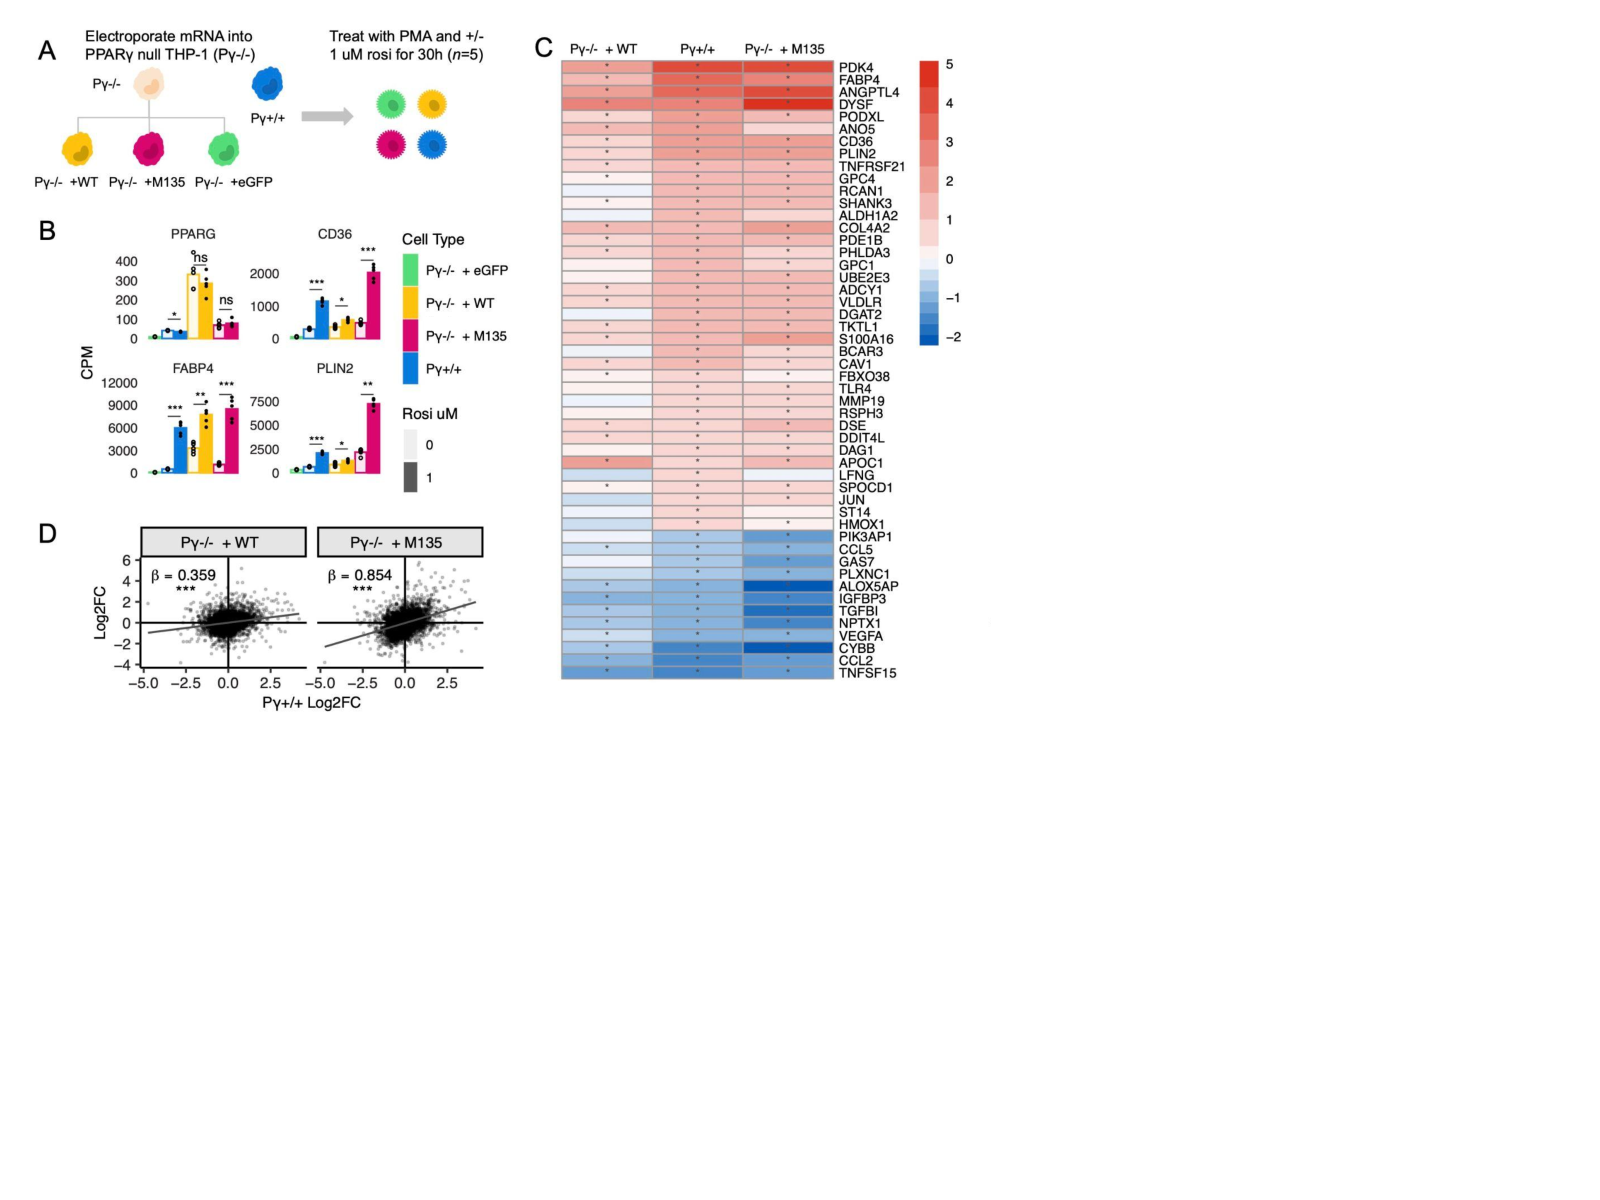
\includegraphics[width=\textwidth]{1_figures-and-files/Fig3.pdf}
    \caption[PPAR$\gamma$ M135 more potently activates ligand stimulated gene expression as compared to WT.]{\textbf{PPAR$\gamma$ M135 more potently activates ligand stimulated gene expression as compared to WT.} A. PPAR$\gamma$ WT and M135 mRNA, along with control eGFP mRNA, were generated through in vitro transcription and electroporated into PPAR$\gamma$ null (P$\gamma$-/-) THP-1 monocytes. The electroporated cells and wild-type THP-1s (P$\gamma$+/+) were differentiated into macrophages and treated with +/- 1 uM rosiglitazone (rosi) for 30 hours before protein and RNA were collected (n=5/condition). B. RNA-seq expression in counts per million (CPM) of PPARG and selected PPAR$\gamma$ target genes. In response to rosiglitazone treatment, P$\gamma$-/- +M135 activates CD36 and PLIN2 with greater fold change than P$\gamma$-/- +WT and P$\gamma$+/+. * Benjamini-Hochberg corrected (BH) p$<$0.01, ** BH p$<$1e-4, *** BH p$<$1e-8. C. Heatmap of log2-fold change (log2FC) in response to rosiglitazone for each cell type of the top 50 differentially expressed genes (DEGs) in P$\gamma$+/+ THP-1s, as ranked by p-value. Asterisks (*) indicate DEGs changing in the same direction with BH corrected p $<$ 0.05. D. Scatterplot of all 1779 P$\gamma$+/+ DEG log2FC values, comparing the log2FC in P$\gamma$+/+ to the log2FC in P$\gamma$-/- +WT and P$\gamma$-/- +M135. Regression slopes ($\beta$) are significant (p $<$ 2e-16, ***) for both, but the P$\gamma$-/- +M135 transcriptional response more closely recapitulates P$\gamma$+/+.
    }\label{fig:3 PPARgamma M135 as a ligand stimulated transactivator}
\end{figure}

To comprehensively evaluate if M135 generated a stronger agonist-induced transcriptional response than WT in P$\gamma$-/- cells, we performed a series of differential expression analyses. We first identified the top-ranked PPAR$\gamma$ target genes as defined by the 50 most significant differentially expressed genes (DEGs) in P$\gamma$+/+ cells +/- rosiglitazone and then compared the log2FC for the same genes across P$\gamma$-/- +WT and P$\gamma$-/- +M135 +/- rosiglitazone (\textbf{Figure 1.3C}). Of the top 50 P$\gamma$+/+ DEGs, 46 were also differentially expressed in P$\gamma$-/- +M135 (p$<$0.05, same sign log2FC), whereas only 33 were differentially expressed in P$\gamma$-/- +WT. Moreover, at several key genes, including \(PDK4\), \(DYSF\), \(ANGPTL4\), \(ALOX5AP\), and \(CYBB\)\cite{De_Morree2013-dh,Pott2012-ji,Keller2018-zv}, P$\gamma$-/- +M135 had a greater activation or repression than P$\gamma$+/+ cells (\textbf{Figure 1.3C}) despite transient and lower PPAR$\gamma$ protein expression per cell (\textbf{Figure A.3}). Across all the P$\gamma$+/+ DEGs (n=1779), the magnitude of gene expression change was more similar for P$\gamma$-/- +M135 cells (slope=0.85) than for P$\gamma$-/- +WT cells (slope=0.36), indicating greater potency of M135 in mediating agonist-induced PPAR$\gamma$ gene expression response than WT (\textbf{Figure 1.3D}).

\begin{figure}[h]
    \centering
    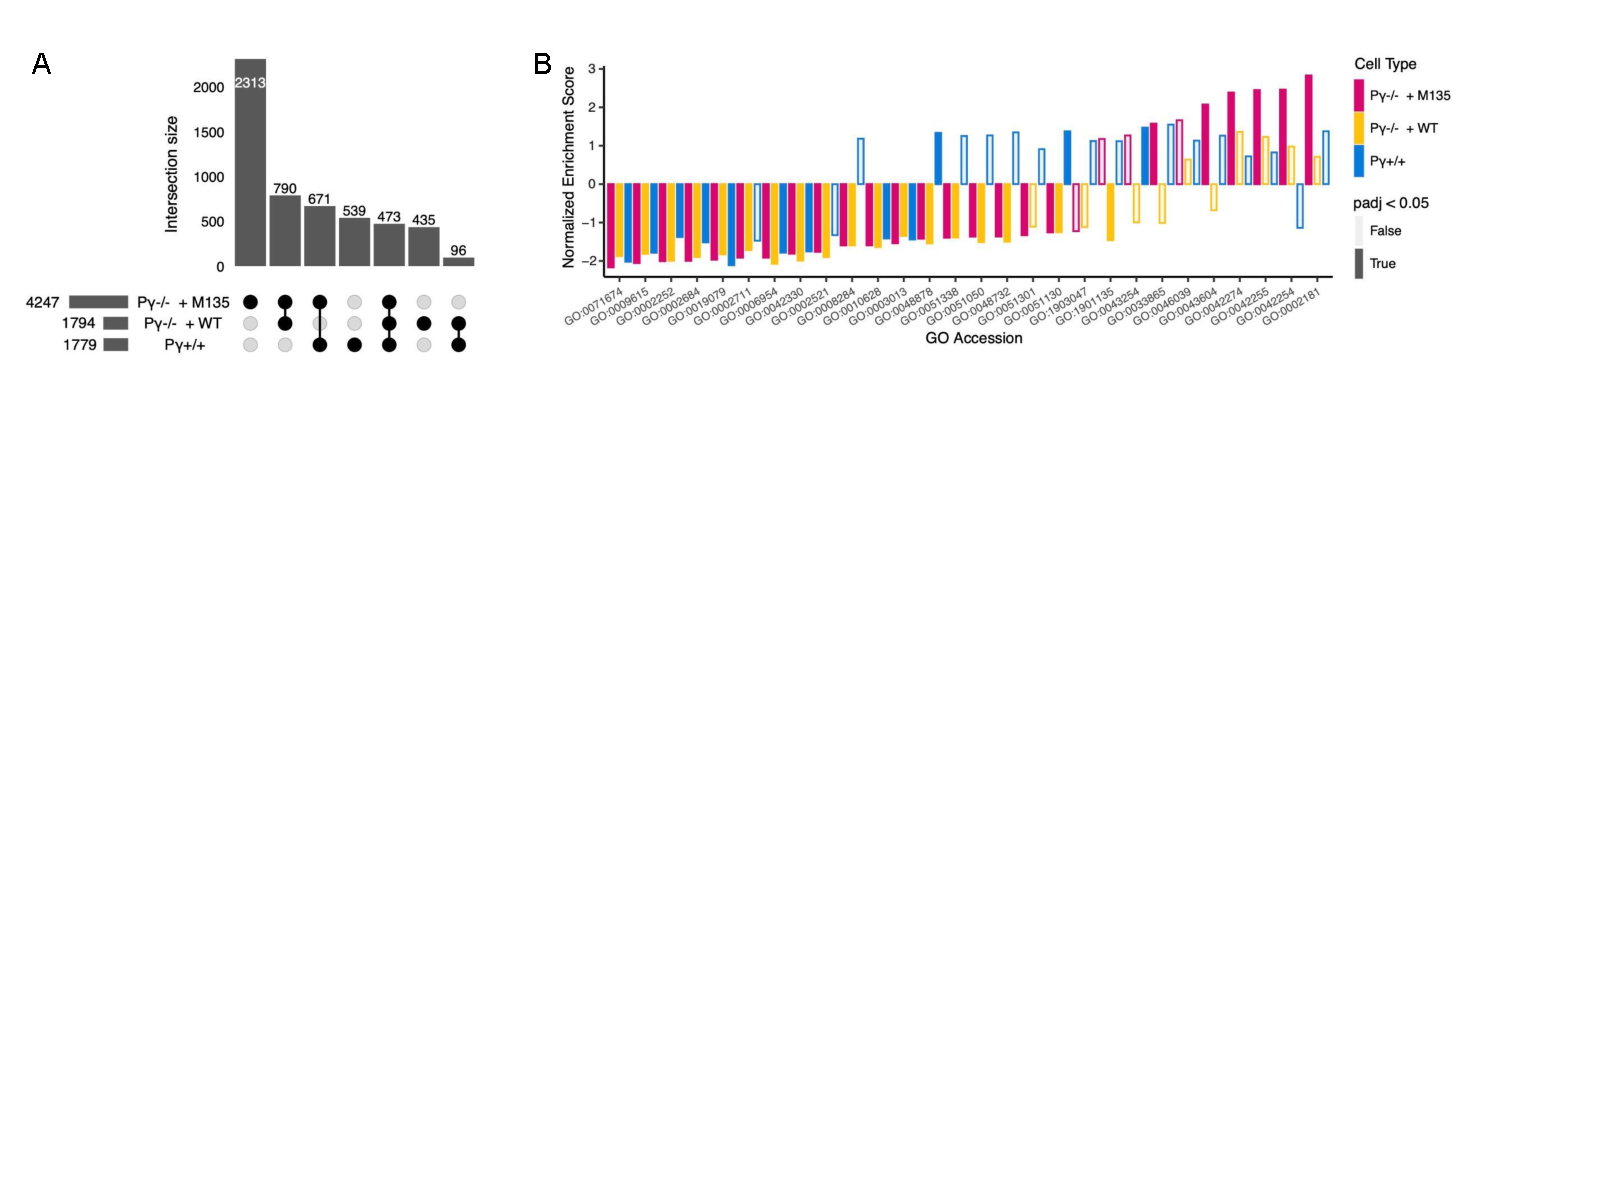
\includegraphics[width=\textwidth]{1_figures-and-files/Fig4.pdf}
    \caption[PPAR$\gamma$ M135 activates more genes in similar biological process pathways as WT.]{\textbf{PPAR$\gamma$ M135 activates more genes in the same biological process pathways as WT.} A. Upset plot of the DEGs per cell type +/- rosiglitazone. Left horizontal bars show total DEGs for each of the three conditions. Filled circles connected by lines indicate intersections among the three conditions and vertical bars show the number of DEGs in the corresponding intersections. B. Normalized enrichment scores in the GO BP pathways for P$\gamma$-/- M135 specific genes. Overall transcriptional pathway activation by P$\gamma$+/+ ,P$\gamma$-/- +WT, P$\gamma$-/- +M135 are similar and consistent.
    }\label{fig:4 PPARgamma M135 has more differentially expressed genes}
\end{figure}

We then queried for DEGs specific to PPAR$\gamma$ M135 to assess if the lack of AF-1 domain in M135 resulted in transactivation/repression of genes not regulated by WT PPAR$\gamma$. In response to rosiglitazone treatment, P$\gamma$-/- +M135 had the greatest number of DEGs (n=4,247, \textbf{Figure 1.4A}) as compared to P$\gamma$-/- +WT (n=1,794) or P$\gamma$+/+ (n=1,779). Of the 4,247 DEGs, 2,313 were exclusive to P$\gamma$-/- +M135 (\textbf{Figure 1.4A}). To understand the gene expression programs captured by these putative M135-specific genes, we performed gene set overrepresentation analysis\cite{Chang2006-im,Yu2012-gb} among the Gene Ontology Biological Process (GO BP) pathways\cite{Ashburner2000-df,Gene_Ontology_Consortium2021-fn} and found 28 overrepresented pathways that were confirmed to be altered by rosiglitazone treatment in M135 complemented cells (p$<$0.05; \textbf{Table A.2}). Among these, 21/28 were similarly altered, although to a lesser degree, by rosiglitazone treatment in either WT-electroporated cells or P$\gamma$+/+ THP-1s (\textbf{Figure 1.4B}). The most enriched result, GO:0002181, is the cytoplasmic translation biological process pathway, and rosiglitazone has been recently found to induce ribosomal transcription in adipocytes\cite{De-Siqueira2024-uz}. Taken together, these analyses suggest that PPAR$\gamma$ M135 regulates similar gene expression programs as WT, but more potently when induced by rosiglitazone, perhaps due to de-repression from the loss of the N-terminal AF-1 domain\cite{Mosure2022-tw}.

%%%%%%%%%%%%%%%%%%%%%%%%%%%%%%%%%%%%%%%%%%%%%%%%%%%%%%%%%%%%%%%%%%%%%%%%%%%%%%%%
\section{Discussion}
%%%%%%%%%%%%%%%%%%%%%%%%%%%%%%%%%%%%%%%%%%%%%%%%%%%%%%%%%%%%%%%%%%%%%%%%%%%%%%%%

In this study, we report and characterize the function of a novel isoform of PPAR$\gamma$ (M135), lacking the AF-1 domain, that can be generated from an alternative downstream translational start site in the second coding exon of \(PPARG\) (chr3:12381414 hg38). We show that PPAR$\gamma$ M135 is transcriptionally active, ligand inducible, and a more potent transactivator than full-length WT PPAR$\gamma$.  

Our finding that PPAR$\gamma$ M135 has increased transactivation potential and is beneficial to metabolic health in vivo aligns with prior studies investigating both naturally occurring and synthetic PPAR$\gamma$ variations. Previous investigators have observed that constructs deleting the N-terminus of PPAR$\gamma$ increase transcriptional potency compared with full-length PPAR$\gamma$ in NIH 3T3 cells\cite{Tontonoz1994-ds,Hummasti2006-rm}. Subsequent work demonstrated that a MAPK phosphorylation site at PPAR$\gamma$ p.S112 inhibits the transactivation function of PPAR$\gamma$\cite{Adams1997-cf}, and PPAR$\gamma$ p.S112A, which lacks the phosphorylation site, is more transcriptionally active\cite{Adams1997-cf,Hu1996-mb,Camp1997-nf}. Additionally, the missense variant PPAR$\gamma$2 p.P12A (rs1801282), which has been robustly associated with a reduced risk of type 2 diabetes in humans\cite{Altshuler2000-kl}, was found to weaken the interaction between PPAR$\gamma$ and its corepressor NCoR, resulting in increased transcriptional activity of PPAR$\gamma$ target genes and improved insulin sensitivity in mice\cite{Heikkinen2009-vb}. Consistent with this mechanism, we find that metabolic syndrome severity scores (METSS) decreases per p.P12A allele carried at the rs1801282 locus. Furthermore, SUMOylation at p.K107 inhibits ligand-induced transactivation of PPAR$\gamma$ targets\cite{Pascual2005-ki}, and removing that modification in mice increased insulin sensitivity without increasing adiposity in mice\cite{Katafuchi2018-jw}. Altogether, these studies illustrate that impairing the AF-1 domain increases PPAR$\gamma$ activity and insulin sensitivity. 

The major limitation of our study is the use of an in vitro cell model. Our experiments were conducted using the THP-1 macrophage cell line which, although human, is not equivalent to in vivo macrophages. However, previous investigations have shown concordant cellular responses between THP-1 monocytes and adipocytes across functional \(PPARG\) variants\cite{Majithia2016-bm,Agostini2018-bx,Majithia2014-op} providing a measure of confidence that these models are suitable for studying genetic variation in \(PPARG\). Furthermore, PPAR$\gamma$ is active in additional tissues including muscle and liver that may have additional metabolic consequences\cite{Norris2003-hi,Gavrilova2003-gb}. These could be the subject of future investigation to fully dissect the metabolic consequences of PPAR$\gamma$ M135.

In summary, we report on PPAR$\gamma$ M135, a novel isoform of \(PPARG\) arising from a downstream alternative translational start site (chr3:12381414 hg38), that is a more potent ligand-inducible transactivator than full-length PPAR$\gamma$. This work points to a new mechanism to activate PPAR$\gamma$ by inhibition of the AF-1 domain that could potentially lead to more effective treatments for insulin resistance-related disorders.

%%%%%%%%%%%%%%%%%%%%%%%%%%%%%%%%%%%%%%%%%%%%%%%%%%%%%%%%%%%%%%%%%%%%%%%%%%%%%%%%
\section{Research Design and Methods}
%%%%%%%%%%%%%%%%%%%%%%%%%%%%%%%%%%%%%%%%%%%%%%%%%%%%%%%%%%%%%%%%%%%%%%%%%%%%%%%%

\subsection{Cell Culture}
Cell suspensions from the human monocytic leukemia cell line THP-1 (ATCC \#TIB-202) were cultured in growth media (RPMI 1640 (Gibco, \#22400089) + 10\% heat-inactivated FBS (Sigma- Aldrich, \#F2442) + 1\% PenStrep (Gibco, \#15140122) + 0.1\% 2-Mercaptoethanol (BME; Sigma-Aldrich, \#M6250)). In all experiments, cells were differentiated with 50 ng/mL phorbol 12-myristate 13-acetate (PMA; Sigma-Aldrich, \#P1585) and PPAR$\gamma$ activation was stimulated with 1uM rosiglitazone (Cayman Chemicals, \#71740).

\subsection{Generation of the pooled CRISPR library}
To study the effect of insertions and deletions (indels) across \(PPARG\), guide RNAs (sgRNAs) were designed using CRISPick\cite{Doench2016-za}, ordered as premixed oligos from IDT, phosphorylated, annealed, and ligated into the lentiCRISPRv2 vector (Addgene \#52961) through Golden Gate cloning\cite{Engler2008-in}. The plasmids were transformed and sequenced for verification. Lentivirus was generated following manufacturer protocols (Mirus Bio \#2304) and used to infect THP-1 cells at MOI=0.3 to minimize doubly infected cells, and the edited cells were selected for using 2 $\mu$g/mL puromycin (Sigma-Aldrich, \#P8833). The distribution and efficiency of infection were assessed as follows. Genomic DNA (gDNA) was extracted from 1 million cells (Qiagen \#51304), split across 4 PCR reactions, amplified (Takara 639208), and loaded onto the iSeq (Illumina), and the reads were deconvolved with PoolQ 3.3.2 (Broad Institute; \url{https://portals.broadinstitute.org/gpp/public/software/poolq}), which showed a 96.8\% completeness with a maximum of 100x difference between the most over-sequenced guide and the least.

\subsection{Pooled CRISPR experimental assay}
To assess the effect of indels across \(PPARG\) on its ability to activate a downstream target, the edited THP-1 cells were sorted, alongside wildtype (P$\gamma$+/+) THP-1s and PPAR$\gamma$ null (P$\gamma$-/-) THP-1s, for expression of CD36. To activate PPAR$\gamma$, the cells were treated with 50 ng/mL PMA for 72 hours and 1 $\mu$M rosiglitazone for 48 hours. The cells were immunostained for CD36 (Miltenyi Biotec, \#130-095-472). Stained cells were sorted using FACS (BD FACSAria II) into two bins: high and low expression of CD36, based on thresholds set by the P$\gamma$+/+ and P$\gamma$-/- cells. 5 independent sorting experiments were performed, sorting approximately 150,000 cells per bin per replicate. To identify and quantify the \(PPARG\) variants in each bin, the methods detailed above were used to extract gDNA, amplify, and sequence. To quantify the effect of each sgRNA on PPAR$\gamma$ function, an enrichment score was generated. The reads for each sorted sample were normalized by library depth, and enrichment was calculated by taking the log2 of the ratio of CD36+ normalized counts to CD36- normalized counts for each sgRNA. 

\subsection{Saturation mutagenesis frameshift analysis}
To determine the impact of indels at each codon of \(PPARG\), a function score for each codon was calculated based on previously published methods\cite{Majithia2016-bm}. The function score is analogous to the CD36+/CD36- enrichment score described above.

\subsection{Generation of monoclonal cell lines}
The endonuclease Cas9 and guides Int-sgRNA, Ex1-sgRNA, and Ex3-sgRNA (\textbf{Table A.1}) were introduced into THP-1 cells by lentiviral transduction. The transduced THP-1 cells were sorted one cell per well into 96-well plates (BD FACSAria II) in growth media supplemented with 50\% conditioned media (RPMI media harvested from healthy cells at $\sim$70\% confluence for 48 hours post the previous passage, clarified by centrifugation at 1000 x g for 10 minutes and then passed through a 0.2 $\mu$m sterile filter to remove any cell debris) and expanded. All cell lines were sequenced to confirm genomic edits and zygosity by Sanger sequencing of genomic DNA.

\subsection{Detecting PPAR\texorpdfstring{$\gamma$}{gamma} isoforms}
Cells were lysed using RIPA lysis buffer (Millipore Sigma, \#20-188), and protease inhibitor (Roche, \#04693132001), and protein concentration was determined. Equal amounts of proteins were separated by 4-12\% Bis-Tris Gels (Invitrogen, \#NP0336) with the SeeBlue Plus2 Prestained Protein Standard (Invitrogen, LC5925) and subsequently blotted on 0.45 um nitrocellulose membrane (Bio-Rad, \#1620115). The membrane was incubated with antibodies against PPAR$\gamma$ for N-terminus (1:1000 Cell Signaling Technology (CST) \#2435, RRID:AB\_2166051), for C-terminus recognition (1:1000 CST \#2443, RRID:AB\_823598), and cyclophilin B (1:1000 CST Cat\# 43603, RRID:AB\_2799247), followed by anti-rabbit secondary antibody conjugated with DyLight 680 Fluorescent dye (1:20,000 CST \#5366, RRID:AB\_10693812). Finally, the membranes were visualized with Odyssey CLx imager (LI-COR).

\subsection{Cycloheximide chase}
3 million THP-1 cells were seeded per well in a 6-well plate and differentiated for 24 hours with 50 ng/mL PMA. Translation was arrested with 5 uM cycloheximide, and cells were collected after 0, 0.5, 1, and 2 hours of treatment (n=3). Fifteen $\mu$g protein from each sample were loaded into a western blot with the PageRuler Plus Prestained Protein Ladder (Thermo \#26619) and processed as detailed above with primary antibodies CST \#2443 for PPAR$\gamma$ and CST \#41185 for actin. Intensities for the PPAR$\gamma$1, PPAR$\gamma$ M135, and actin bands were quantified on Image Studio, and the PPAR$\gamma$ intensities for each sample were normalized to its corresponding actin intensity to control for the amount of protein. For each PPAR$\gamma$ isoform, the percentage relative to baseline was calculated by dividing the normalized PPAR$\gamma$ intensity by the mean of that isoform at 0 hours. For each sample, the ratio of PPAR$\gamma$1 to PPAR$\gamma$ M135 was obtained by dividing the percentage relative to baseline of PPAR$\gamma$1 by that of PPAR$\gamma$ M135. Statistical analysis was performed with one-way ANOVA with a Tukey post hoc test.

\subsection{In vitro transcription}
To evaluate the complementation of PPAR$\gamma$ using wildtype (WT) and M135 PPAR$\gamma$ isoforms, in vitro transcription was performed as previously described\cite{Heinz2018-mp}. Briefly, cDNA constructs were amplified from plasmids containing the PPAR$\gamma$2 sequence using primers that introduce a T7 promoter and AG on the 5$^{\prime}$ end and a 179-nt poly (A) on the 3$^{\prime}$ end (PPAR$\gamma$ WT FWD: 5$^{\prime}$-GAATTTAATACGACTCACTATAAGGAAATACGCCACCATGGGTGAAACTCTGGGAGAT-3$^{\prime}$; M135 FWD: 5$^{\prime}$-GAATTTAATACGACTCACTATAAGGAAATACGCCACCATGGCAATTG\newline AATGTCGTGTCT-3$^{\prime}$, REV1: 5$^{\prime}$-CTAGGACATCGCAGTCTGCACCTAGTACAAGTCCTTG\newline TAGATCTCCTG-3$^{\prime}$; REV2: 5$^{\prime}$- (T)179-CTAGGACATCGCAGTCTGCAC-3$^{\prime}$). To generate capped, polyadenylated mRNA, PCR products were phenol-chloroform extracted and in vitro transcribed with T7 RNA Polymerase HiScribe Mix (NEB \#E2040S), CleanCap Reagent AG (TriLink \#N-7113) and 5-methoxyuridine triphosphate (TriLink \#N-1093-5) instead of UTP. The mRNA was precipitated with lithium chloride and resuspended in water.

\subsection{Luciferase assay}
Transcriptional activity of the PPAR$\gamma$ isoforms was tested in HEK293 cells using a PPAR promoter driven luciferase reporter (PPREx3-luc, Addgene plasmid \# 1015; a gift from Bruce Spiegelman). HEK293 cells were seeded 20,000/well and co-transfected with a mixture of 10 ng Renilla (pGL4.75), 10 ng PPREx3-LUC, and 100 ng PPAR$\gamma$ mRNA using Lipofectamine 3000 (Thermo L3000001) for 48 hours. Rosiglitazone treated samples were incubated with 0.5 uM for 16 hours. Firefly and Renilla luciferase activity was quantified by using the Dual Luciferase Assay System (Promega \#E1910), as described by the manufacturer. Luciferase activity was normalized for moles of mRNA transfected.

\subsection{Creating THP-1 cells with exogenous isoforms}
To introduce the \(PPARG\) IVT mRNA into P$\gamma$-/- THP-1 cells, the transcripts were electroporated into cells on the BioRad XCell in a 4 mm cuvette with one 400 V, 5 ms square wave pulse. To match PPAR$\gamma$ protein expression, 2 $\mu$g of M135 mRNA and 8 $\mu$g of WT mRNA were used for each electroporation of 3 million cells (n=5 per cell type). After each electroporation, the cells were split into 3 for protein collection, treatment with 50 ng/uL PMA, and treatment with 50 ng/uL PMA and 1 $\mu$M rosiglitazone. To study the transcriptomes of these cells, RNA was extracted from the latter two conditions (Zymo \#R1050) and sent for library preparation (Illumina Stranded mRNA Prep) and 100 bp paired-end sequencing (25 million reads/sample on the NovaSeq S4).

\subsection{Transcriptomic analysis of THP-1 cell types}
 Raw sequencing reads were aligned to the reference hg38 using Kallisto with default parameters\cite{Bray2016-zt} to generate gene counts per cell. Analysis was performed in R 4.1.3. EdgeR 3.36.0 and limma-voom (limma v3.50.1) were used to filter and normalize reads for library size and perform differential expression\cite{Robinson2010-qx,Law2014-yh}. UpSetR v1.4.0 was applied to visualize the intersections in differentially expressed genes (DEGs) between the P$\gamma$+/+, P$\gamma$-/- +M135, and P$\gamma$-/- +WT cell lines in response to rosiglitazone\cite{Lex2014-lr,Conway2017-hp}. To study changes in gene sets, overrepresentation analyses and enrichment analyses were performed in fgsea v1.20.0\cite{Korotkevich2021-ra}.

\subsection{Treatment of monoclonal THP-1 cells for qPCR}
Ex1-sgRNA -/- and Int-sgRNA +/+ monoclonal cells were seeded in 12-well plates with 750,000 cells per well. 12 wells of each genotype were differentiated with 50 ng/mL PMA for a total of 72 hours, with 6 wells of each genotype additionally receiving 1 uM rosiglitazone in the last 24 hours. RNA was extracted (Zymo \#R1050) for qPCR. Two independent rounds of seeding and collection were performed.

\subsection{Quantitative PCR for THP-1s}
Reverse transcription was performed with the SuperScript III First-Strand Synthesis System (ThermoFisher 18080051) following manufacturer’s instructions. Gene expression was analyzed using the iTaq Universal SYBR Green Supermix (Bio-Rad 1725121) with \(GAPDH\) as the housekeeping gene. Cycle threshold values (Ct) were analyzed using the $\Delta\Delta$Ct method\cite{Livak2001-va}. Briefly, following outlier removal, technical replicates (n=2) were averaged, and $\Delta$Ct values were calculated for each biological replicate along with their mean and standard error (n=6 for Figure 1.2C). Relative expression (fold-change) was calculated as \[2^{-\Delta\Delta Ct}\] setting a reference condition $\Delta$Ct from differentiated Int-sgRNA THP-1s as a calibrator.

%%%%%%%%%%%%%%%%%%%%%%%%%%%%%%%%%%%%%%%%%%%%%%%%%%%%%%%%%%%%%%%%%%%%%%%%%%%%%%%%
\section{Acknowledgements}
%%%%%%%%%%%%%%%%%%%%%%%%%%%%%%%%%%%%%%%%%%%%%%%%%%%%%%%%%%%%%%%%%%%%%%%%%%%%%%%%

We are deeply grateful to Angela Liu for technical assistance. 
 
\subsection{Author Contributions}
A.R.M conceived the study. X.D., K.M.-L., and A.R.M. designed the experiments. X.D., K.M-L., S.H., R.D., G.B., R.H., K.G., C.D.A.S., J.F., S.Heinz and A.R.M. generated/acquired and analyzed the data. X.D., K.M.-L., S.H., R.D., G.B., R.H., J.F., S.Heinz, and A.R.M. were involved in data interpretation. X.D., K.M-L. and A.R.M. drafted the initial manuscript. All authors were involved in manuscript revision. A.R.M is the guarantor of this work and, as such, had full access to all the data in the study and takes responsibility for the integrity of the data and the accuracy of the data analysis.

\subsection{Duality of Interest}
The authors declare no competing interests.  

\subsection{Funding}
This work was supported by grants from the National Institute of Diabetes and Digestive and Kidney Diseases (1R01DK123422 and R01HL159760 to A.R.M, 1R01DK125490 to J.F and A.R.M) and a UCSD/UCLA Pilot and Feasibility grant (P30 DK063491 to A.R.M). This publication includes data generated at the UC San Diego IGM Genomics Center utilizing an Illumina NovaSeq 6000 that was purchased with funding from a National Institutes of Health SIG grant (\#S10 OD026929).\\ 

\noindent Chapter 1, in full, was modified for this thesis from the material in Diabetes 2025. The dissertation/thesis author was the primary investigator and author of this paper. I would like to acknowledge my co-authors for the research in Chapter 1, Karen Mendez-Lara, Siqi Hu, Rachel Diao, Guru Bhavimani, Ruben Hernandez, Kimberly Glass, Camila De Arruda Saldanha, Jason Flannick, Sven Heinz, and Amit Majithia.

\bibliographystyle{unsrtnat}
\bibliography{bib_1.bib}
\chapter{PPAR\texorpdfstring{$\gamma$}{gamma} M135 has the capacity to be insulin sensitizing
}\label{chap:chapter 2}

%%%%%%%%%%%%%%%%%%%%%%%%%%%%%%%%%%%%%%%%%%%%%%%%%%%%%%%%%%%%%%%%%%%%%%%%%%%%%%%%
\section{Introduction}
%%%%%%%%%%%%%%%%%%%%%%%%%%%%%%%%%%%%%%%%%%%%%%%%%%%%%%%%%%%%%%%%%%%%%%%%%%%%%%%%

The \(PPARG\) gene encodes PPAR$\gamma$, a nuclear hormone receptor that is a master regulator of adipocyte differentiation and is the molecular target of thiazolidinediones (TZDs), a class of drugs that decrease insulin resistance\cite{Tontonoz2008-pe,Yki-Jarvinen2004-ba}. TZDs are potent insulin sensitizers that treat type 2 diabetes, cardiovascular disease (CVD), and non-alcoholic fatty liver disease (NAFLD)\cite{Kernan2016-fd,Inzucchi2016-ni,Musso2017-xi}, but they cause serious side effects, including fluid retention\cite{Yki-Jarvinen2004-ba}. A novel isoform of PPAR$\gamma$, named PPAR$\gamma$ M135, was identified and characterized in Chapter 1. This isoform demonstrated increased transactivation potential in response to TZD treatment compared to wild-type PPAR$\gamma$2.

PPAR$\gamma$ M135 differs from canonical isoforms PPAR$\gamma$1 and PPAR$\gamma$2 with its lack of the autonomous activation-function domain 1 (AF-1); the DNA binding domain (DBD) and ligand binding domain (LBD) are present in all three isoforms. Multiple loss-of-function (LOF) mutations in \(PPARG\) occurring in the DBD and LBD have been shown to cause familial partial lipodystrophy type 3 (FPLD3), a Mendelian genetic syndrome characterized by insulin resistance, metabolic syndrome, and gluteofemoral fat loss\cite{Savage2003-wm,Agostini2006-hc,Broekema2019-nz}. These pathogenic FPLD3 mutations establish the clinical significance of the PPAR$\gamma$ DBD and LBD, but form the tip of the iceberg in human protein-coding variants found in \(PPARG\)\cite{Majithia2014-op}. In previous work, we have identified hundreds of protein-coding variants in \(PPARG\) occurring in all protein domains including the AF-1 domain\cite{Majithia2016-bm}. As with FPLD3, those that cause LOF in the DBD and LBD increased insulin resistance and type 2 diabetes risk. We observed no apparent clinical impact of LOF variants in the AF-1 domain, leaving in question its function in human metabolic health.

In this study, we expand on the insulin sensitizing activity of PPAR$\gamma$ M135. We find that PPAR$\gamma$ M135 demonstrates enhanced ligand-inducible transcriptional and functional activity compared to wild-type (WT) in a human preadipocyte cell line. To evaluate the clinical consequence of this model, we identified and analyzed human carriers of \(PPARG\) variants that impair AF-1 function, finding that these variants increase PPAR$\gamma$ function and decrease metabolic syndrome severity in people who carry them. Taken together, our study nominates AF-1 domain inhibition as a new targetable mechanism to activate PPAR$\gamma$.

%%%%%%%%%%%%%%%%%%%%%%%%%%%%%%%%%%%%%%%%%%%%%%%%%%%%%%%%%%%%%%%%%%%%%%%%%%%%%%%%
\section{Results}
%%%%%%%%%%%%%%%%%%%%%%%%%%%%%%%%%%%%%%%%%%%%%%%%%%%%%%%%%%%%%%%%%%%%%%%%%%%%%%%%

\subsection{Human preadipocytes that generate PPAR\texorpdfstring{$\gamma$}{gamma} M135 more potently upregulate target genes than WT preadipocytes}

As many of the major metabolic effects of \(PPARG\) on human physiology occur in adipocytes\cite{Majithia2014-op}, we evaluated if adipocytes could also generate PPAR$\gamma$ M135 and to what functional consequence. We targeted a human preadipocyte cell line (Simpson-Golabi-Behmel Syndrome (SGBS)\cite{Wabitsch2001-fx}) with disruptions in Exon 1, Exon 3, and a \(PPARG\) intron (Ex1-sgRNA2 cut site at hg38 chr3:12379716, Ex3-sgRNA chr3:12392733, and Int-sgRNA chr3:12363492, \textbf{Figure 2.1A}). The edited cells were treated with inducers of adipocyte differentiation and examined for PPAR$\gamma$ protein expression, target gene expression, and adipocyte differentiation efficiency. After four days of differentiation, we were able to detect both PPAR$\gamma$ WT and M135 in Exon 1 targeted cells, whereas Exon 3 targeted cells expressed no PPAR$\gamma$, and control cells only expressed WT PPAR$\gamma$ (\textbf{Figure 2.1B, C}). These results indicated that, like THP-1 macrophages, SGBS adipocytes are capable of alternatively generating PPAR$\gamma$ M135 in response to disruptive mutations targeted to Exon 1.

\clearpage
\begin{figure}[!ht]
    \centering
    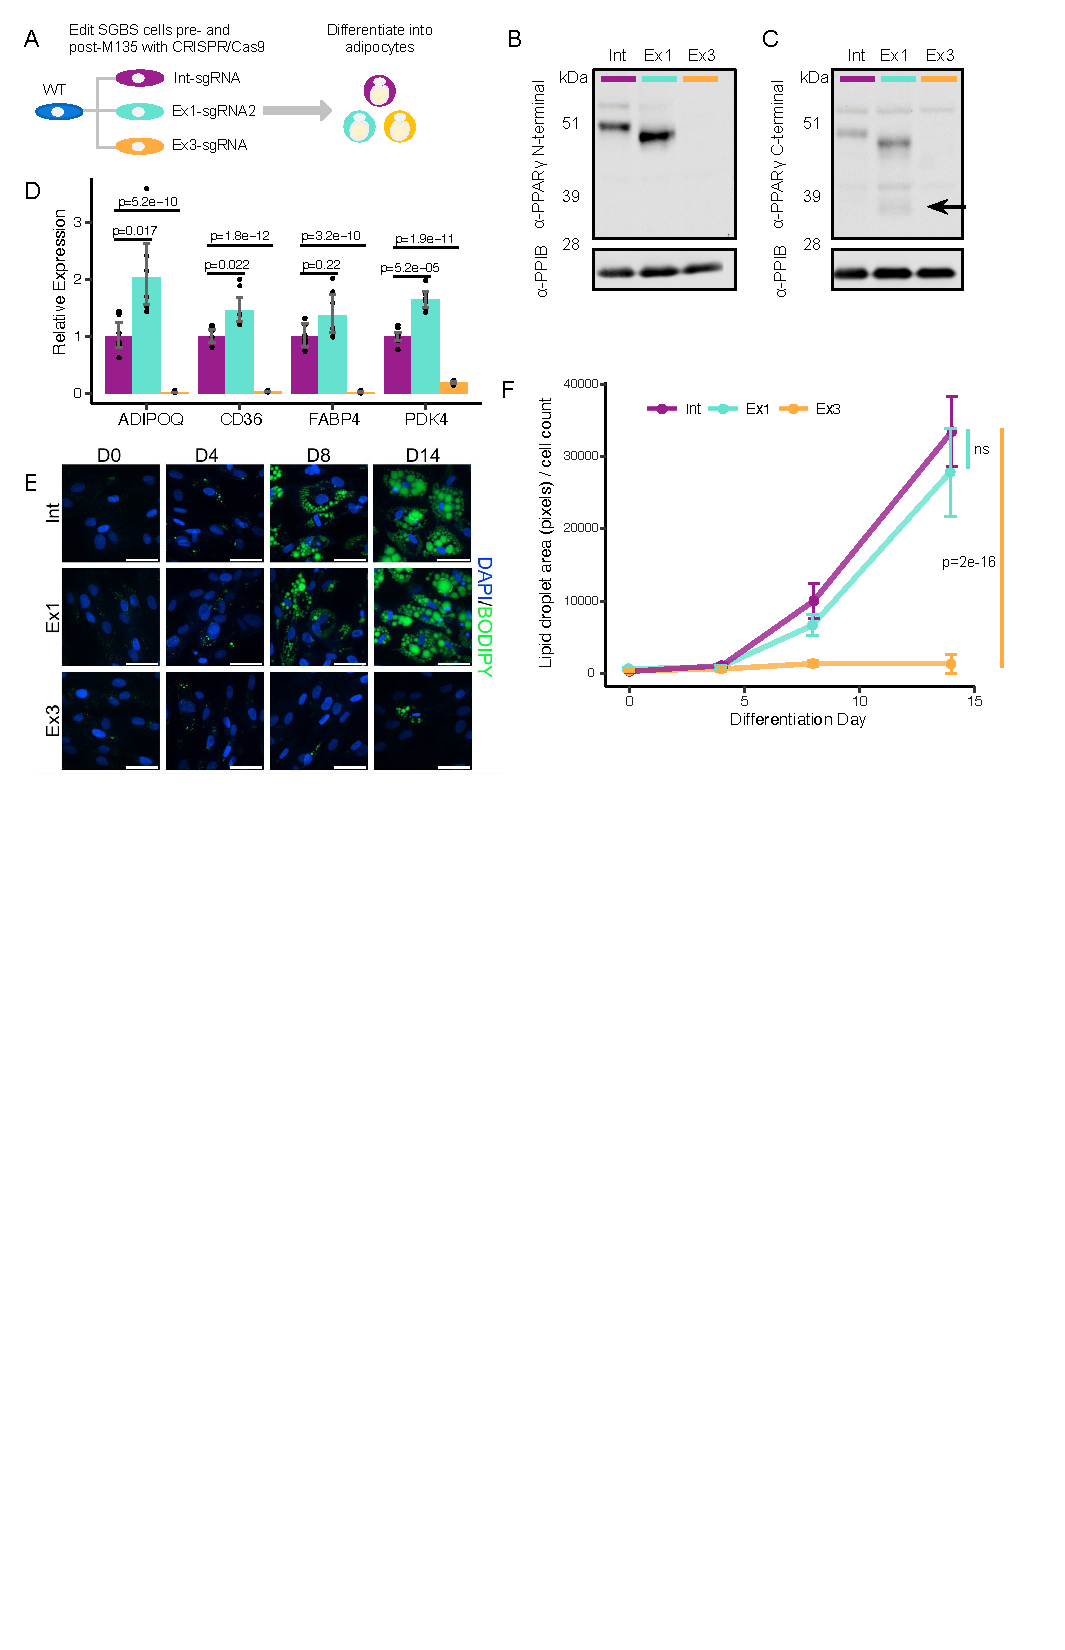
\includegraphics[width=\textwidth]{2_figures-and-files/Fig1.pdf}
    \caption[Human preadipocytes generate PPAR$\gamma$ M135 and more potently upregulate target genes than WT]{\textbf{Human preadipocytes generate PPAR$\gamma$ M135 and more potently upregulate target genes than WT.} \textbf{A.} Simpson-Golabi-Behmel Syndrome (SGBS) cells were transduced with a vector containing Cas9 and a sgRNA targeting \(PPARG\) Exon 1 (chr3:12379716), Exon 3 (chr3:12392733), or an intron (chr3:12363492). The preadipocytes were differentiated into adipocytes. \textbf{B,} \textbf{C.} Western blot for the N-terminus (B, left) and C-terminus (C, right) of PPAR$\gamma$ in SGBS preadipocytes treated with \(PPARG\) targeting constructs (A) at 4 days post-differentiation. The Ex1 targeted preadipocytes generate PPAR$\gamma$ M135 at 40 kDa (arrow), while the Ex3 targeted cells do not express any PPAR$\gamma$. Exon 1 targeted cells also express a band $\sim$50 kDA, consistent with translation initiation at PPAR$\gamma$ p.M53. \textbf{D.} Expression of PPAR$\gamma$ target genes at 4 days of differentiation by qPCR.\@ Ex1 targeted cells expressed higher levels of \(ADIPOQ\), \(CD36\), and \(PDK4\) compared to control. Ex3 edited cells minimally express all PPAR$\gamma$ target genes. N=6 replicates per sample, p-values from linear models of $\Delta$ Ct (see Methods for more details). \textbf{E,} \textbf{F.} Differentiation time-course for Int, Ex1, and Ex3 targeted SGBS cells at days 0, 4, 8, and 14. Cells were fixed and stored in PBS on their respective collection dates, stained on day 14 for nuclei (DAPI, blue) and lipids (BODIPY, green), and imaged. \textbf{E.} Imaged at 40x magnification. Ex1 SGBS differentiate on par with Int, and Ex3 SGBS do not accumulate lipids. Scale bar is 50 $\mu$m. \textbf{F.} Quantification of lipid accumulation in SGBS cells. The data was log-normalized and regressed against genotype and differentiation day to determine the effect of genotype. Ex1 was not different from Int (p=0.933), and Ex3 resulted in a significantly different pace (p = 2e-16).
    }\label{fig:PPARgamma M135 in human adipocytes}
\end{figure}
\clearpage

To evaluate the ability of preadipocytes expressing PPAR$\gamma$ M135 to activate PPAR$\gamma$ target genes, we queried gene expression of several targets during early adipocyte differentiation (\textbf{Figure 2.1D}). SGBS preadipocytes that express PPAR$\gamma$ M135 increase expression of \(CD36\) (p=0.022) and \(PDK4\) (p=5.2e-5) to a significantly greater extent than PPAR$\gamma$ WT expressing cells and showed a trend towards increased expression of \(FABP4\) (p=0.22). Furthermore, we examined adiponectin (\(ADIPOQ\)), an adipokine and PPAR$\gamma$ target specific to adipocytes\cite{Combs2002-sr}, and found it also to be significantly upregulated by PPAR$\gamma$ M135 expressing adipocytes (p=0.017) compared to WT (\textbf{Figure 2.1D}). Cells targeted at Exon 3, which expressed no PPAR$\gamma$, failed to upregulate the expression of any of these genes. 

Finally, we characterized the ability of PPAR$\gamma$ M135 expressing SGBS cells to mature into adipocytes and accumulate lipids during differentiation (\textbf{Figure 2.1E, F}). Exon 1 targeted, PPAR$\gamma$ M135 expressing SGBS differentiated and accumulated lipids at the same rate as control PPAR$\gamma$ WT expressing cells (p=0.933), whereas Exon 3 targeted cells had significantly reduced lipid accumulation (p=2e-16). These analyses show that like macrophages, human preadipocytes can generate the PPAR$\gamma$ M135 isoform, and the truncated isoform is fully functional in driving differentiation into mature, lipid-laden adipocytes.

\subsection{PPAR\texorpdfstring{$\gamma$}{gamma} M135 enhances adipocyte insulin response compared to WT}

To isolate the effect of PPAR$\gamma$ M135, we transduced P$\gamma$-/- SBGS cells (i.e. Ex3-sgRNA targeted cells) with doxycycline-inducible WT PPAR$\gamma$2 cDNA (SGBS P$\gamma$-/- +WT) or PPAR$\gamma$ M135 cDNA (SGBS P$\gamma$-/- +M135) transgenes and evaluated differentiation/ lipid accumulation and insulin response (\textbf{Figure 2.2A}). These cells only express PPAR$\gamma$ (WT or M135) when treated with doxycycline (\textbf{Figure 2.2B}) and differentiate to a similar degree only when PPAR$\gamma$ is induced (p=0.56, \textbf{Figure 2.2C, D}).

\clearpage
\begin{figure}[ht]
    \centering
    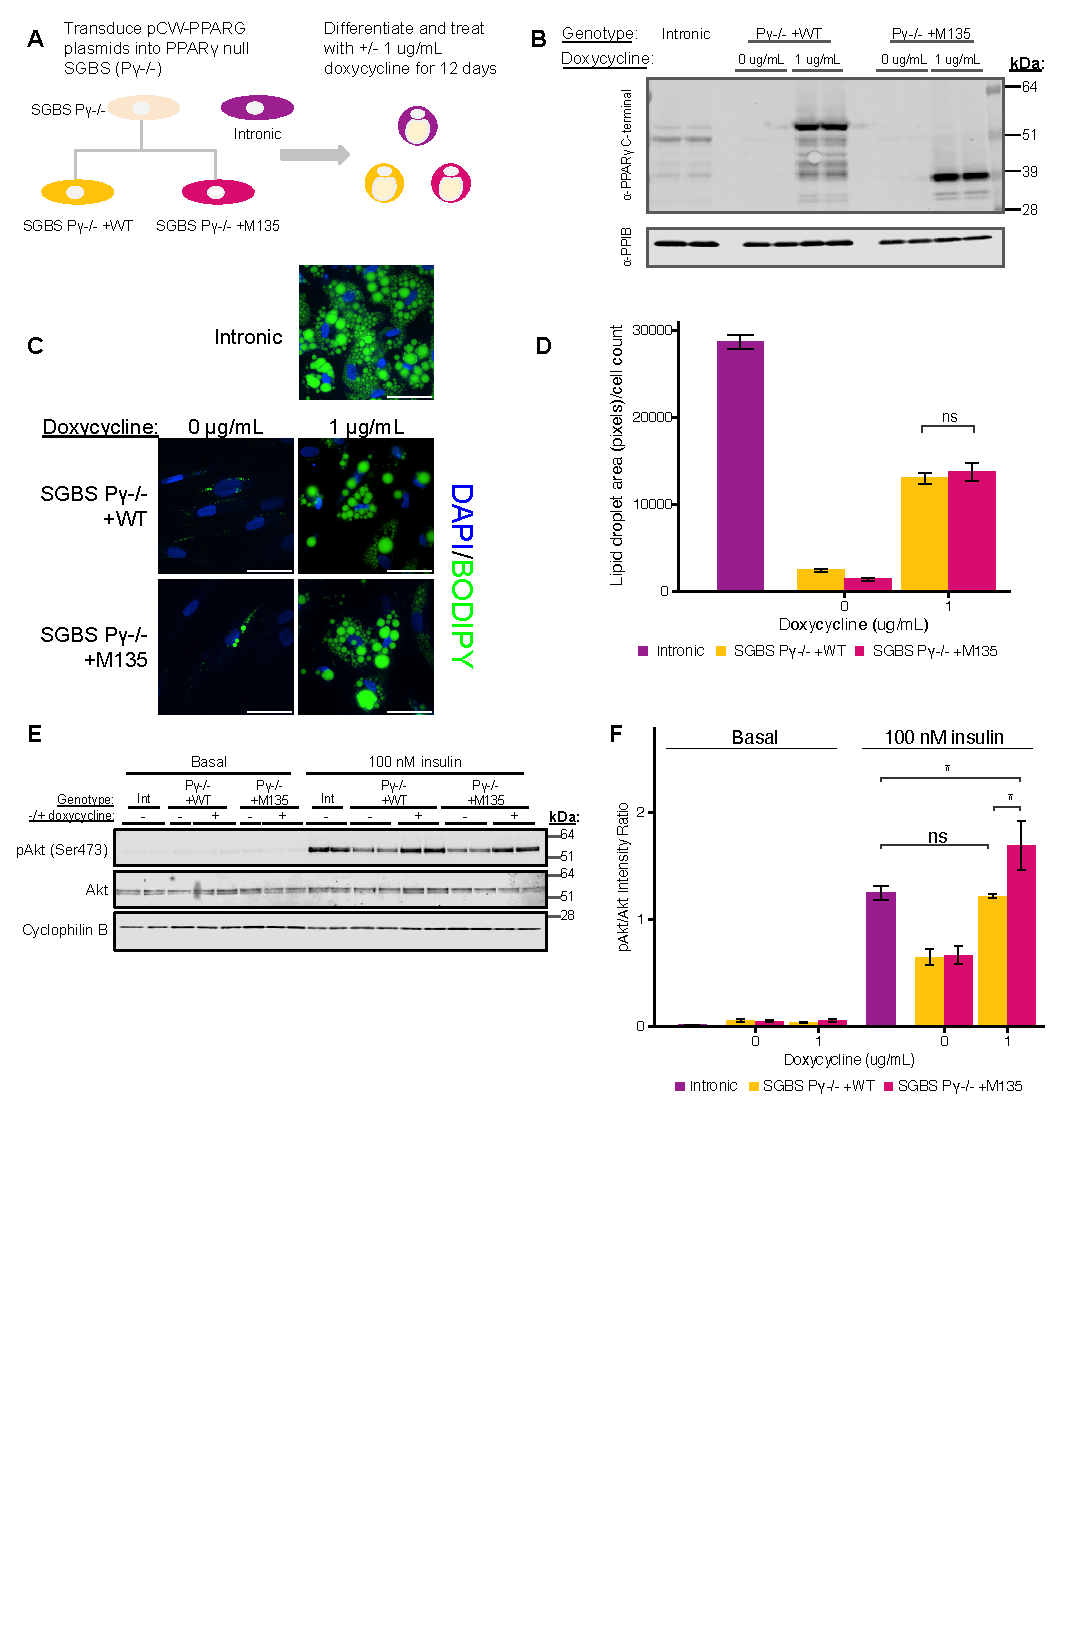
\includegraphics[width=0.8\textwidth]{2_figures-and-files/Fig2.pdf}
    \caption[PPAR$\gamma$ M135 enhances adipocyte insulin response compared to WT.]{\textbf{PPAR$\gamma$ M135 enhances adipocyte insulin response compared to WT.} \textbf{A.} SGBS P$\gamma$-/- cells were transduced with doxycycline-inducible vectors expressing PPARG WT and M135. The preadipocytes were differentiated and treated +/- doxycycline. \textbf{B.} PPAR$\gamma$ expression in the SGBS cells. SGBS P$\gamma$-/- cells with PPARG transgenes only express PPAR$\gamma$ when treated with doxycycline. \textbf{C,} \textbf{D.} Intronic, SGBS P$\gamma$-/- +WT, and SGBS P$\gamma$-/- +M135 cells were differentiated for 12 days, fixed, stained for nuclei (DAPI, blue) and lipid accumulation (BODIPY, green), and imaged. \textbf{C,} Imaged at 40x magnification. PPAR$\gamma$ M135 is sufficient to induce differentiation and lipid uptake in SGBS P$\gamma$-/- cells. Scale bar is 50 $\mu$m. \textbf{D.} Quantification of lipid accumulation. SGBS P$\gamma$-/- +M135 cells accumulate the same amount of lipids as SGBS P$\gamma$-/- +WT (n=12 images/well, 4 wells per genotype, p=0.56, t-test). \textbf{E,} \textbf{F.} Intronic, SGBS P$\gamma$-/- +WT, and SGBS P$\gamma$-/- +M135 cells were treated +/+ doxycycline, +/+ 100 nM insulin for 20 minutes and immunoblotted for phosphorylated Akt (pAkt) and total Akt (n=4 biological replicates). \textbf{E.} Representative immunoblot. \textbf{F.} The pAkt/Akt intensity ratios were significantly different across the conditions (ANOVA p=1.33e-13). Pairwise comparisons are highlighted between the 100 nM insulin stimulated samples for SGBS P$\gamma$-/- +M135 and SGBS P$\gamma$-/- +WT cells treated with 1 ug/mL doxycycline (Tukey HSD p=0.025, *), SGBS P$\gamma$-/- +M135 + doxycycline and Intronic (p=0.045, *), and SGBS P$\gamma$-/- +WT + doxycycline and Intronic (p=0.99, ns). 
    }\label{fig:PPARgamma M135 insulin response}
\end{figure}
\clearpage

To assess insulin response control (intronic), SGBS P$\gamma$-/- +WT and SGBS P$\gamma$-/- +M135 were differentiated, stimulated with insulin and immunoblotted for phosphorylated Akt (S473; pAkt) and total Akt. In response to insulin all cell lines phosphorylate Akt and the response is augmented in doxycycline treated SGBS P$\gamma$-/- +WT and SGBS P$\gamma$-/- +M135 (ANOVA p=1.33e-13, Tukey HSD $\mathrm{p}_{\mathrm{WT, doxycycline}}$=3.67e-8, $\mathrm{p}_{\mathrm{M135, doxycycline}}$=3.43e-11, \textbf{Figure 2.2E, F}). Notably, PPAR$\gamma$ M135 expressing adipocytes show increased insulin stimulated AKT phosphorylation compared to both WT(p=0.025) and control SGBS (p=0.045), indicating an enhanced insulin response.

\subsection{Missense mutations that impair AF-1 function increase PPAR\texorpdfstring{$\gamma$}{gamma} transactivation and may protect against metabolic syndrome in human carriers}

Next, we sought to evaluate the potential in vivo consequence of nonsense mutations in the \(PPARG\) sequence prior to chr3:12381414 by identifying human carriers of such mutations and performing genotype:phenotype correlation under the hypothesis that carriers would not exhibit insulin resistance given the enhanced molecular activity of PPAR$\gamma$ M135 from AF-1 domain deletion. Across biobanks and databases comprising over 1.2 million individuals with sequencing at the \(PPARG\) locus, we only found seven carriers of nonsense mutations prior to chr3:12381414 (\textbf{Table B.1}). Among these, two had no evidence of metabolic syndrome or insulin resistance past 50 years of age, one had type 2 diabetes, but no ascertainment of insulin resistance or metabolic syndrome, and four had no available phenotypic information.

As the number of human pre-M135 nonsense mutation carriers was insufficient to make robust inferences, we turned to carriers of \(PPARG\) missense variants to test the hypothesis that genetic variants abrogating AF-1 domain function would enhance PPAR$\gamma$ activity and thereby increase insulin sensitivity in vivo (\textbf{Figure 2.3A}). While missense variants are not equal to having the M135 isoform, they can model how disruptions to the AF-1 domain affect PPAR$\gamma$ activity in vivo. We rationalized this hypothesis based on recent data that the AF-1 domain intramolecularly binds to the ligand binding domain (LBD) of PPAR$\gamma$, and this interaction inhibits ligand-dependent activity\cite{Mosure2022-tw}. 

\clearpage
\begin{figure}[t]
    \centering
    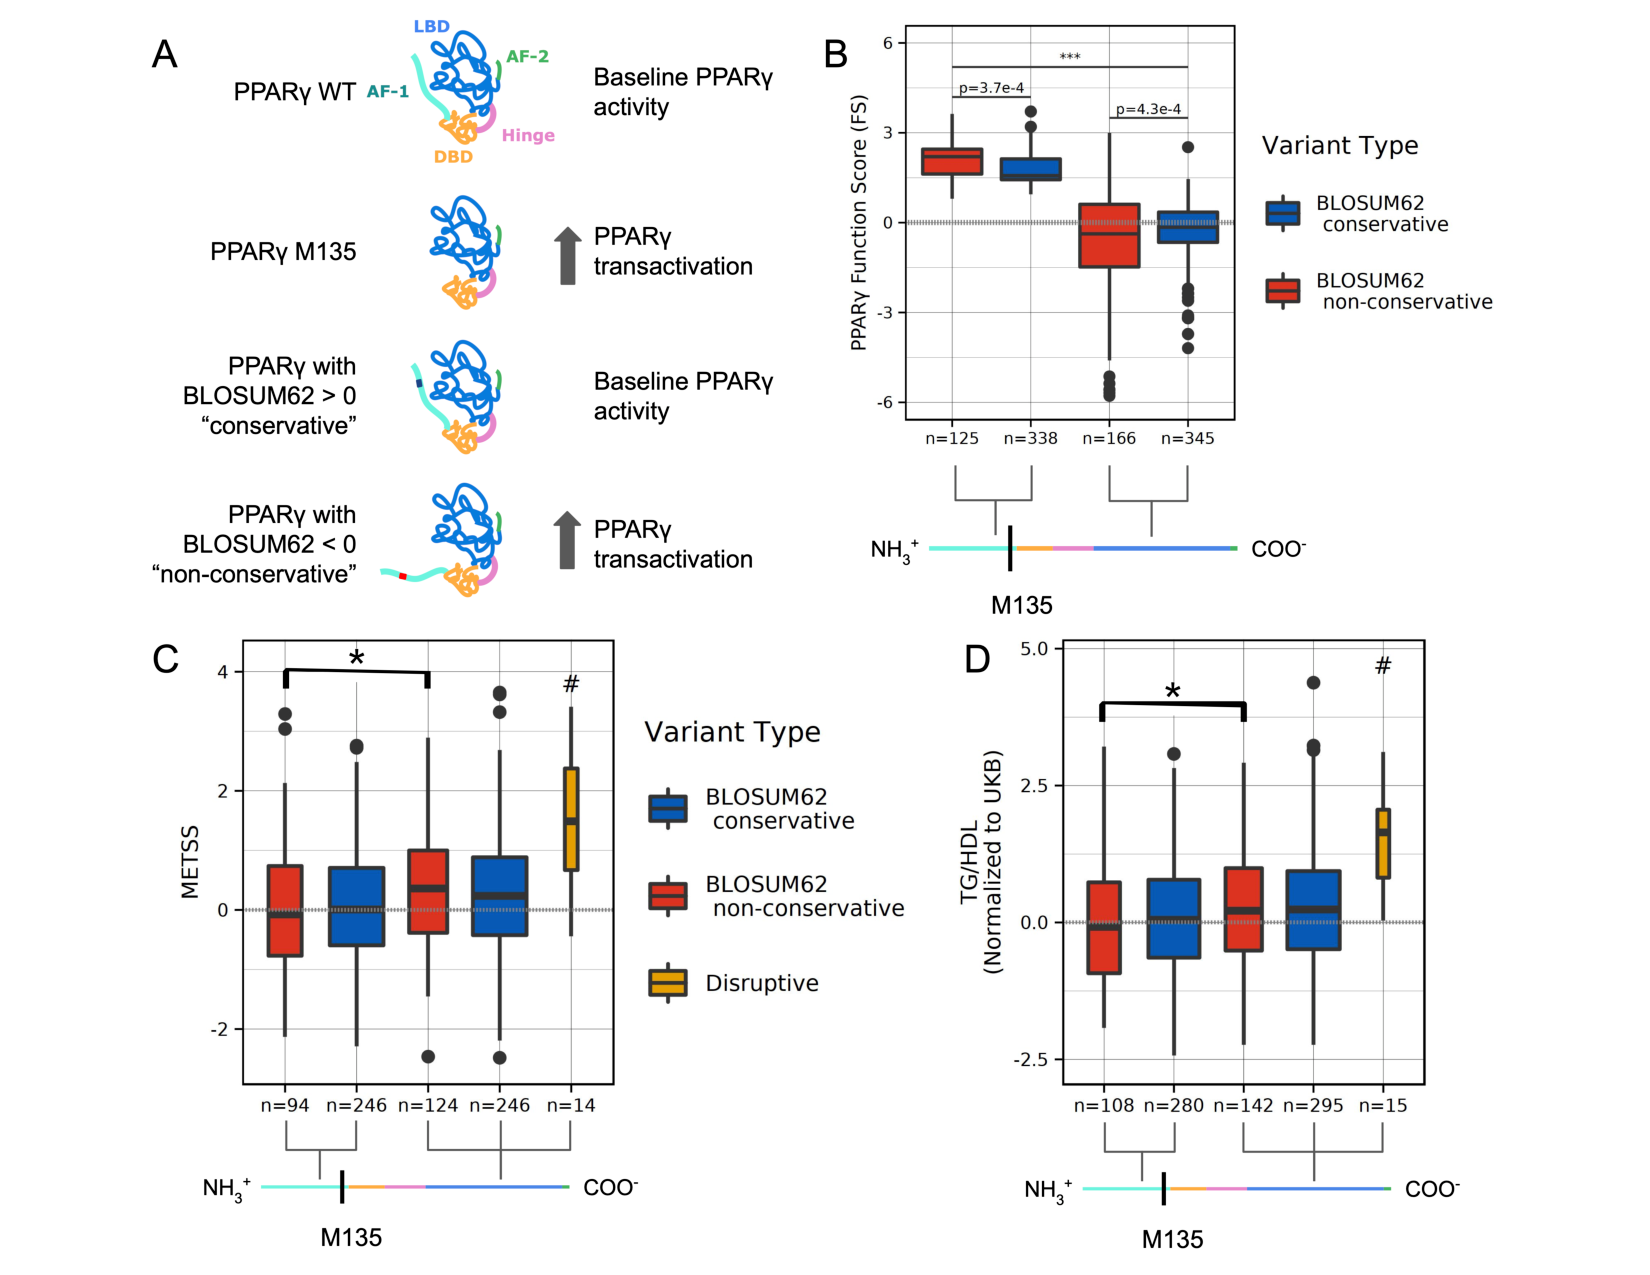
\includegraphics[width=\textwidth]{2_figures-and-files/Fig3.pdf}
    \caption[Human carriers of variants in PPAR$\gamma$ that impair the AF-1 domain are protected from metabolic dysfunction.]{\textbf{Human carriers of variants in PPAR$\gamma$ that impair the AF-1 domain are protected from metabolic dysfunction.} \textbf{A.} Cartoon representation of AF-1 hypothesis. Cyan: AF-1, Orange: DNA-binding domain (DBD), Pink: Hinge, Blue: Ligand-binding domain (LBD), Green: AF-2. Protein cartoon modeled after the PPAR$\gamma$ crystal structure shown in Mosure et al., 2022. \textbf{B.} Function scores (FS) for \(PPARG\) missense variants (MAF $<$ 0.001) from the UK Biobank (UKB) by position (i.e. pre-/post-M135), and evolutionary conservation (conservative: BLOSUM62 $<$ 0, nonconservative: BLOSUM62 $>$ 0) category. All pairwise comparisons between categories are significant by ANOVA (p $<$ 2e-16, ***) and Tukey HSD. \textbf{C.} Metabolic syndrome severity score (METSS) by position and conservation, as in B. There is a significant difference between pre-/post-M135 non-conservative METSS (*, p=0.016, Welch’s t). \# indicates that the disruptive carriers are significantly different from every other category by ANOVA (p=4.1e-6) and Tukey HSD (p$<$8.6e-4). \textbf{D.} TG/HDL, a measurement for insulin resistance, is plotted by position and conservation. The carriers of disruptive variants have significantly higher TG/HDL (\#, ANOVA p=7.31e-7, Tukey HSD p$<$1.1e-4), and there is a significant difference between pre-/post-M135 non-conservative variant carriers (*, p=0.017, Welch’s t).
    }\label{fig:Human carriers of PPARG variants}
\end{figure}
\clearpage

We identified all carriers of rare (MAF $<$ 0.001) protein-coding variants in \(PPARG\) in the UK Biobank (UKB, n=454,787)\cite{Backman2021-kd} and analyzed the cellular function and amino acid position of the variants carried in relation to the insulin sensitivity-related phenotypes of the individuals carrying them. To quantify PPAR$\gamma$ activity, we leveraged the PPAR$\gamma$ function score (FS) derived from our previously published deep mutational scan, in which every possible missense variant was scored by its transactivation of CD36\cite{Majithia2016-bm}. We found 1,250 carriers of 260 unique rare, protein-coding \(PPARG\) variants and partitioned them by pre-/post- M135 and by the BLOSUM62 substitution matrix, which quantifies the tolerance of amino acids to substitution across evolutionary distance\cite{Henikoff1992-jo}. Variants were categorized as “conservative” (BLOSUM62 $>$ 0) or “non-conservative” (BLOSUM62 $<$ 0). Non-conservative substitutions in AF-1 ($\mathrm{FS}_{\mathrm{median}}$=2.21) have higher PPAR$\gamma$ FS than conservative substitutions ($\mathrm{FS}_{\mathrm{median}}$=1.56), while non-conservative substitutions post-M135 in the DBD and LBD ($\mathrm{FS}_{\mathrm{median}}$=-0.158) show decreased PPAR$\gamma$ FS relative to conservative mutations ($\mathrm{FS}_{\mathrm{median}}$=-0.376; ANOVA p$<$2e-16, adjusted p$<$0.005 for each pairwise comparison by Tukey HSD; \textbf{Figure 2.3B}). These data support the hypothesis that missense variants disrupting AF-1 domain function increase the transcriptional activity of PPAR$\gamma$.

To quantify insulin sensitivity in these \(PPARG\) missense variant carriers, we computed a per-individual metabolic syndrome severity score (METSS), a measure of insulin sensitivity determined from waist circumference, systolic blood pressure, serum triglycerides, HDL cholesterol, and serum glucose (HbA1c), using methods analogous to those previously published\cite{Gurka2014-ib,Cavero-Redondo2019-ce,Agarwal2012-qu}. We calculated METSS for the 368,911 individuals in the UKB who had all five measurements ascertained, including 908 of the 1250 carriers of rare, protein-coding \(PPARG\) variants (\textbf{Figure B.1a, b}). Of the rare \(PPARG\) missense variant carriers in the UKB, 340 pre-M135 and 370 post-M135 carriers had computable METSS values. As with the PPAR$\gamma$ function score analysis above (\textbf{Figure 2.3B}), we partitioned each group into conservative and non-conservative BLOSUM62 to examine the effect of each variant category on METSS (\textbf{Figure 2.3C}). Under the model that amino acid substitutions that abrogate AF-1 domain function would increase PPAR$\gamma$ activity and thereby decrease METSS, we hypothesized that non-conservative missense variants in AF-1 (pre-M135) would confer lower METSS as compared to conservative amino acid substitutions that would preserve AF-1 function. Conversely, we expected that non-conservative mutations post-M135 in the DBD or LBD would increase METSS, as is the case for lipodystrophy\cite{Jeninga2009-pt}. As a positive control, we identified carriers of post-M135 disruptive (i.e. nonsense and frameshift causing) \(PPARG\) variants (n=14) in our cohort and found their METSS score to be significantly elevated ($\mathrm{METSS}_{\mathrm{median}}$=1.5, \textbf{Figure 2.3C}) compared to other \(PPARG\) variant carriers (ANOVA p=4.1e-6, Tukey p$<$8.6e-4) and the general UKB population (Welch’s t, p=1.1e-4). We observed an ordinal trend with non-conservative, pre-M135 variant carriers having the lowest METSS ($\mathrm{METSS}_{\mathrm{median}}$=-0.079) followed by conservative, pre-M135 ($\mathrm{METSS}_{\mathrm{median}}$=0.0064), conservative, post-M135 ($\mathrm{METSS}_{\mathrm{median}}$=0.24) and finally non-conservative, post-M135 ($\mathrm{METSS}_{\mathrm{median}}$=0.36). The difference between pre- and post-M135 non-conservative variant carriers is significant (Welch’s t, p=0.016).

We performed a similar analysis alternatively utilizing the serum triglyceride to HDL cholesterol (TG/HDL) ratio as a surrogate measure of insulin sensitivity\cite{Oliveri2024-bz,DeForest2024-ex}. The trends observed with METSS were consistent in the TG/HDL results: carriers of post-M135 disruptive (i.e. nonsense and frameshift causing) \(PPARG\) variants (n=15) had the highest values compared to other \(PPARG\) variant carriers ($\mathrm{TG/HDL}_{\mathrm{median}}$=1.65, \textbf{Figure 2.3D}; ANOVA p=7.31e-7, Tukey HSD p$<$1.1e-4), and the non-conservative, pre-M135 variant carriers had the lowest TG/HDL (n=108, $\mathrm{TG/HDL}_{\mathrm{median}}$= +0.080). The difference between pre- and post-M135 non-conservative variant carriers is significant (Welch’s t, p=0.017).

\clearpage
\begin{table}[t]
    \centering
    \caption[METSS statistics for carriers of \texorpdfstring{\(PPARG\)}{PPARG} Pro12Ala (rs1801282) in the UKB.]{\textbf{METSS statistics for carriers of \texorpdfstring{\(PPARG\)}{PPARG} Pro12Ala (rs1801282) in the UKB.}  Increasing alleles of Ala are associated with decreasing METSS.
  }
    \begin{tabular}{|c|c|c|c|c|}
    \hline
        Genotype & Carriers (n) & Median METSS & Mean METSS & Standard Deviation \\ \hline
        Pro/Pro & 287785 & 0.0035 & 0.0087 & 1.0015 \\ \hline
        Pro/Ala & 75619 & -0.0326 & -0.026 & 0.9947 \\ \hline
        Ala/Ala & 5263 & -0.0839 & -0.0964 & 0.9796 \\ \hline
    \end{tabular}
\end{table}

We separately analyzed the well known \(PPARG\) p.P12A variant (rs1801282, MAF=\newline 0.1050) that is associated with decreased type 2 diabetes risk\cite{Altshuler2000-kl} and occurs frequently in the general population. Under the above partitioning scheme, \(PPARG\) p.P12A would be classified as pre-M135, non-conservative (FS = 1.3, BLOSUM62 score = +1). Carriers of the p.P12A allele (n=80,882) in the UKB had significantly decreased METSS (per allele effect size = +0.039, p=2e-16, \textbf{Table 2.1}, \textbf{Figure B.1c}). These data are suggestive of a model in which AF-1 disrupting variants (both common and rare) can improve insulin sensitivity in vivo.


%%%%%%%%%%%%%%%%%%%%%%%%%%%%%%%%%%%%%%%%%%%%%%%%%%%%%%%%%%%%%%%%%%%%%%%%%%%%%%%%
\section{Discussion}
%%%%%%%%%%%%%%%%%%%%%%%%%%%%%%%%%%%%%%%%%%%%%%%%%%%%%%%%%%%%%%%%%%%%%%%%%%%%%%%%

In this study, we characterize the function of PPAR$\gamma$ M135 in adipocytes and model its effects with human genetics. We show that PPAR$\gamma$ M135 is more transcriptionally active and insulin sensitizing than WT PPAR$\gamma$ in response to exogenous agonism in human preadipocytes. Finally, we characterize metabolic syndrome severity in human carriers of \(PPARG\) variants, demonstrating that variants that abrogate AF-1 domain function potentially protect carriers from insulin resistance. Our data support a model for in vivo de-repression of PPAR$\gamma$ in humans that is metabolically beneficial.  

Regarding therapeutic development, our data suggest an opportunity to physiologically activate PPAR$\gamma$ through a mechanism distinct from thiazolidinediones (TZDs), which bind the LBD. While TZDs have demonstrated benefits in treating/preventing type 2 diabetes and CVD events\cite{Lebovitz2019-oe,dreamteam2006-hz}, they cause side effects such as weight gain\cite{Yki-Jarvinen2004-ba}. Much pharmacological development has focused on identifying molecules that are selective PPAR$\gamma$ modulators (SPPARMs) that would provide insulin sensitization without side effects, but most SPPARM molecules target the LBD of PPAR$\gamma$\cite{Higgins2010-tv} and still show appreciable rates of weight gain and fluid retention compared to placebo\cite{DePaoli2014-hi}. Our study nominates the AF-1 domain as a therapeutic target that is mechanistically distinct from TZDs and SPPARMs, as removing the AF-1 would de-repress rather than activate PPAR$\gamma$. Accordingly, our data show that adipocytes engineered to produce PPAR$\gamma$ M135 express higher levels of adiponectin, an insulin sensitizing adipokine\cite{Berg2001-oq,Stern2016-kw}. Further supporting this proposal are the murine models of human and synthetic \(PPARG\) variants that increase PPAR$\gamma$ activity via impairing AF-1 (p.P12A\cite{Heikkinen2009-vb}, p.S112A\cite{Rangwala2003-hm}, p.K107\cite{Katafuchi2018-jw}) which show enhanced insulin sensitivity compared to WT littermates.

In summary, we report on PPAR$\gamma$ M135, a novel isoform of \(PPARG\) arising from a downstream alternative translational start site (chr3:12381414 hg38), that is a more potent ligand-inducible transactivator than full-length PPAR$\gamma$. This work points to a new mechanism to activate PPAR$\gamma$ by inhibition of the AF-1 domain that could potentially lead to more effective treatments for insulin resistance-related disorders.

%%%%%%%%%%%%%%%%%%%%%%%%%%%%%%%%%%%%%%%%%%%%%%%%%%%%%%%%%%%%%%%%%%%%%%%%%%%%%%%%
\section{Research Design and Methods}
%%%%%%%%%%%%%%%%%%%%%%%%%%%%%%%%%%%%%%%%%%%%%%%%%%%%%%%%%%%%%%%%%%%%%%%%%%%%%%%%

\subsection{Generation and characterization of SGBS cell lines edited at the \texorpdfstring{\(PPARG\)}{PPARG} locus}

SGBS cells were seeded at 10,000 cell/cm2 and transduced with the endonuclease Cas9 and guides Int-sgRNA, Ex1-sgRNA2, and Ex3-sgRNA. Infected cells were selected with puromycin and differentiated 7 days after infection as we have previously published\cite{Jiao2019-ng}. Staining and quantification of cells for lipid accumulation with BODIPY (lipid) and DAPI (nuclei) after differentiation was performed as we have done previously\cite{Majithia2014-op}. Quantitative PCR for day 4 differentiation was performed as detailed above for THP-1s. Data were analyzed in aggregate over two separate transductions (batches), each with three biological replicates. To account for multiple biological replicates in two separate batches, relative expression (fold-change) was determined by a linear model of $\Delta$Ct \textasciitilde Genotype (Int, Ex1, Ex3) + Transduction\_Batch, using the intronic targeted samples as reference (i.e. calibrator). The estimate, error, and p-values for Genotype were used as the $\Delta\Delta$Ct, standard error, and p-values, respectively, with relative expression calculated as \[2^{-\Delta\Delta\mathrm{Ct}}.\]

\subsection{SGBS rescue experiments}

\(PPARG\) cDNA was synthesized (Twist Bioscience) with synonymous mutations\newline (CCDS2609 c.C594T, c.G603C, c.T610A, c.C511G) to eliminate the Ex3-sgRNA recognition sequence (chr3:12392727-12392749), following the principles of guide-intrinsic mismatch tolerance\cite{Fu2022-jh}. The oligo was PCR amplified to generate cDNA sequences encoding PPAR$\gamma$2 and PPAR$\gamma$ M135. These sequences were cloned into the doxycycline-inducible pCW plasmid (Addgene \#184708) using AgeI-HF (NEB \#M0202S), NheI-HF (NEB \#R3131S), and T4 DNA ligase (NEB \#M0202S). Virus was produced, and SGBS P$\gamma$-/- cells were infected to create the SGBS P$\gamma$-/- +WT and SGBS P$\gamma$-/- +M135 cell lines. Cells were differentiated for 12 days before downstream experiments.

\subsection{Imaging}
Cells were fixed in 4\% PFA for 10 minutes (Fisher Scientific \#50-980-487), permeabilized with 0.1\% Triton X-100 (Sigma Aldrich \#X100) for 10 minutes, then stained with 5 ug/mL DAPI (Sigma Aldrich \#D9542) and 2 ug/mL BODIPY 493/503 (Invitrogen \#D3922) for 30 minutes. Images were acquired using a Nikon BioPipeline spinning disk confocal microscope and analyzed using CellProfiler v4.1.3\cite{Carpenter2006-vm}.

\subsection{Insulin Stimulation}
Day 12 SGBS adipocytes were cultured in insulin-free DMEM F12 for 24 hours prior to stimulation with 100 nM recombinant insulin (Sigma Aldrich \#I9278) for 20 minutes in glucose-free Krebs-Ringer buffer as previously described\cite{Tews2022-am}. Cells were placed on ice and insulin-containing buffer was immediately removed prior to washing with cold PBS and cell collection.

\subsection{Immunoblots for phosphorylated-Akt (pAkt) and Akt}
Protein lysates for the SGBS adipocytes were processed as detailed above, and the membranes were incubated with primary antibodies CST \#2920 (Akt), CST \#4060 (phospho-Akt Ser473), and CST \#43603 (cyclophilin B), followed by fluorescent secondary antibodies CST \#5366, \#5151, and \#5470. Imaging was performed on the Odyssey CLx imager (LI-COR).

\subsection{Human Biobank Data}
UK Biobank (UKB) research was conducted under application numbers 41189 and 51436. Framingham Heart Study (FHS) data was accessed through dbGaP project \#30824, “Study on Genetic Risk Scores for Insulin Resistance and their Relation to Metabolic Diseases,” and the All of Us Researcher Workbench was accessed through the workspace, “Detection and analysis of genetic risk factors for insulin resistance v7.” The 1000G variants were accessed through the public data browser\cite{1000_Genomes_Project_Consortium2015-fz}. The Regeneron Genetics Center Million Exome dataset was accessed through the public variant browser\cite{Sun2023-ty}, which includes data accessed through UKB application 26041. The Regeneron Genetics Center, and its collaborators (collectively, the “Collaborators”) bear no responsibility for the analyses or interpretations of the data presented here. Any opinions, insights, or conclusions presented herein are those of the authors and not of the Collaborators. For all exome sequenced cohorts, variants within the genomic coordinates of \(PPARG\) (chr3: 12287368-12434356 hg38) were extracted, and variant annotation was performed using SnpEff v4.3\cite{Cingolani2012-gd}. Nomenclature used for missense variants is for the canonical \(PPARG\) transcript ENST00000287820.10; protein ENSP00000287820.6. Function scores were obtained from the \(PPARG\) saturation mutagenesis performed by Majithia et al.\cite{Majithia2016-bm}.

\subsection{Metabolic syndrome severity score (METSS)}
To calculate a continuous score for metabolic syndrome severity, the values of the five constituent clinical phenotypes\cite{Gurka2014-ib,Cavero-Redondo2019-ce}, serum HDL cholesterol (field 30760), waist circumference (field 48), serum triglycerides (field 30870), systolic blood pressure (field 4080), and glycated hemoglobin (HbA1c, field 30750), were extracted for all UKB participants who had a complete set of measurements and genetic ancestry data (n=368,911). Systolic blood pressure values were corrected for individuals reported to be taking blood pressure medication by adding 15 mm Hg to the listed measurements\cite{Evangelou2018-wo}, and serum triglyceride values were log-normalized. To incorporate the multiple parameters that define metabolic syndrome into one score, dimensionality reduction through principal component analysis (R 4.1.3 prcomp) was performed on the corrected values of the five phenotypes. The resulting principal components (PCs) were regressed against PPAR$\gamma$ function score (FS), adjusted for age, $\mathrm{age}^2$, and sex, and the significant PCs were combined into the metabolic syndrome severity score (METSS = PC5 + PC4 + PC1). The score was adjusted for the covariates of age, age2, sex, and the first ten principal components of genetic ancestry, and the residuals were normalized across the UKB participants (n=368,911). The final METSS thus has a mean of 0 and standard deviation of 1 across the UKB, and it has a significant effect size when regressed against the PPAR$\gamma$ FS (\textbf{Figure B.1b}).

\subsection{TG/HDL}
Serum HDL cholesterol (field 30760) and serum triglycerides (field 30870) were extracted for all UKB participants who had a complete set of measurements and genetic ancestry data (n=425,472). Serum triglyceride values were log-normalized, and the ratio of TG/HDL was applied. TG/HDL was adjusted for the covariates of age, $\mathrm{age}^2$, sex, and the first ten principal components of genetic ancestry, and the residuals were normalized across the UKB participants (n=425,472).

%%%%%%%%%%%%%%%%%%%%%%%%%%%%%%%%%%%%%%%%%%%%%%%%%%%%%%%%%%%%%%%%%%%%%%%%%%%%%%%%
\section{Acknowledgements}
%%%%%%%%%%%%%%%%%%%%%%%%%%%%%%%%%%%%%%%%%%%%%%%%%%%%%%%%%%%%%%%%%%%%%%%%%%%%%%%%
We would like to thank the All of Us participants, as the All of Us Research Program would not be possible without their partnership. We are grateful to Angela Liu for technical assistance. Microscopy was performed at the Nikon Imaging Center at UCSD with the support of P. Guo and R. Sanchez. This research has been conducted using the UK Biobank Resource under Application Numbers 41189 and 51436. We would like to acknowledge the participants and the contributions made by the UK Biobank (www.ukbiobank.ac.uk) in providing the data and resources used in this study.  

\subsection{Author Contributions}
As this work was derived from the same manuscript, see \ref{chap:chapter 1} for corresponding details.

\subsection{Funding}
This work was supported by grants from the National Institute of Diabetes and Digestive and Kidney Diseases (1R01DK123422 and R01HL159760 to A.R.M, 1R01DK125490 to J.F and A.R.M) and a UCSD/UCLA Pilot and Feasibility grant (P30 DK063491 to A.R.M). This publication includes data generated at the UC San Diego IGM Genomics Center utilizing an Illumina NovaSeq 6000 that was purchased with funding from a National Institutes of Health SIG grant (\#S10 OD026929). The All of Us Research Program is supported by the National Institutes of Health, Office of the Director: Regional Medical Centers: 1 OT2 OD026549; 1 OT2 OD026554; 1 OT2 OD026557; 1 OT2 OD026556; 1 OT2 OD026550; 1 OT2 OD 026552; 1 OT2 OD026553; 1 OT2 OD026548; 1 OT2 OD026551; 1 OT2 OD026555; IAA \#: AOD 16037; Federally Qualified Health Centers: HHSN 263201600085U; Data and Research Center: 5 U2C OD023196; Biobank: 1 U24 OD023121; The Participant Center: U24 OD023176; Participant Technology Systems Center: 1 U24 OD023163; Communications and Engagement: 3 OT2 OD023205; 3 OT2 OD023206; and Community Partners: 1 OT2 OD025277; 3 OT2 OD025315; 1 OT2 OD025337; 1 OT2 OD025276.
\\

\noindent Chapter 2, in full, was modified for this thesis from the material in Diabetes 2025. The dissertation/thesis author was the primary investigator and author of this paper. I would like to acknowledge my co-authors for the research in Chapter 2, Karen Mendez-Lara, Siqi Hu, Rachel Diao, Guru Bhavimani, Ruben Hernandez, Kimberly Glass, Camila De Arruda Saldanha, Jason Flannick, Sven Heinz, and Amit Majithia.

\bibliographystyle{unsrtnat}
\bibliography{bib_2.bib}
\chapter{Establishing the framework to reprogram a preadipocyte cell line into depot-specific adipocytes
}\label{chap:chapter 3}


%%%%%%%%%%%%%%%%%%%%%%%%%%%%%%%%%%%%%%%%%%%%%%%%%%%%%%%%%%%%%%%%%%%%%%%%%%%%%%%%
\section{Introduction}
%%%%%%%%%%%%%%%%%%%%%%%%%%%%%%%%%%%%%%%%%%%%%%%%%%%%%%%%%%%%%%%%%%%%%%%%%%%%%%%%

Adipose tissue is a dynamic endocrine organ that plays a central role in maintaining metabolic homeostasis. Adipose depots are anatomically and functionally diverse, but they are commonly grouped as subcutaneous (SAT) and visceral adipose tissue (VAT). The question of what underlies the differences between these two tissues has been explored through many modalities, including across gene expression\cite{Gesta2006-so,Tchoukalova2010-ea}, protein secretion\cite{Wajchenberg2002-pt,Roca-Rivada2015-ee,Kahn2022-tq}, methylation\cite{McAllan2023-qo}, acetylation\cite{Navarro-Ruiz2022-xi}, triglyceride turnover\cite{Spalding2017-lr}, and ex vivo differentiation\cite{Macotela2012-wy,Laber2023-qe}. The transcriptomic divergence between these depots is sufficiently pronounced that a recent bulk deconvolution tool requires depot-specific architecture to achieve accurate cell-type estimations\cite{Sorek2024-ah}.   

Accumulation of VAT has a two-fold stronger correlation with insulin resistance measures than SAT, including cardiovascular risk factors\cite{Preis2010-eh}, while accumulation of SAT can be regarded as metabolically beneficial\cite{Tran2008-cw}. One prevailing hypothesis of why VAT contributes more to metabolic dysfunction is the portal theory, which proposes that VAT releases free fatty acids (FFAs) and inflammatory cytokines into the liver through the portal vein, thereby impairing hepatic insulin sensitivity; however, current evidence disputes the FFA component and instead supports a primary role for the inflammatory factors\cite{Sakers2022-wb,Item2012-mg}. While the myriad of cell types in adipose tissue all contribute to cytokine secretion, this chapter will focus on adipocytes, whose depot‑specific characteristics remain to be fully explored.   

It is insufficient to only study mature, fatty adipocytes, as their precursors already contain epigenetic differences\cite{Macotela2012-wy}. Even within one depot, different populations of preadipocytes have been found to progress into separate clusters of adipocytes\cite{Ramirez2020-jz}. A recent study examining adipocytes from both VAT and SAT delineated classical adipocytes, defined by enrichment of lipid metabolism pathways, and nonclassical adipocytes, which were enriched in specialized functions such as immune regulation, angiogenesis, fibrosis, and mitochondrial processes\cite{Lazarescu2025-ru}. In pseudotime analysis, nonclassical adipocytes were found between preadipocytes and classical adipocytes, indicating that classical adipocytes are at the end state and have lost specialized functions. Therefore, to fully elucidate the differences between subcutaneous and visceral fat cells, it is essential to perform comparisons throughout adipocyte differentiation.   

To do so, we need a more robust method of studying adipocytes from SAT and VAT. There are existing methods to generate adipocytes from stem cells\cite{Taura2009-is,Noguchi2013-od}, but they do not specify which kind of adipocyte is generated. Rather, the origin of the stem cell impacts the resulting adipocyte. Mesenchymal stem cells (MSCs) collected from SAT differentiate into adipocytes with subcutaneous markers, while MSCs from VAT differentiate into visceral adipocytes\cite{Macotela2012-wy,Mathur2022-fx}. However, visceral adipose depots are difficult to access, while SAT can be collected more easily from procedures such as liposuction\cite{Hafner2014-qp}. Moreover, there are immortalized preadipocyte cell lines\cite{Church2015-gf} and protocols that can be applied to precursors from any adipose depot\cite{Darimont2003-ev}, but the different donor sources, genetic backgrounds, and derivation methods can confound comparisons between these existing models\cite{Kassner2020-mo}. As an additional complication, preadipocytes collected from VAT have limited differentiation potential compared to precursors from SAT, introducing additional difficulties in comparative studies\cite{Dufau2021-vi}. Furthermore, there are commercial sources of primary visceral adipocytes and preadipocytes, but no visceral cell lines\cite{Natsume2020-pr}. Therefore, we propose establishing a method of reprogramming a precursor cell to become a subcutaneous adipocyte (SA) and a visceral adipocyte (VA).   

The field of cell fate determination and reprogramming has expanded with the advent of single cell RNA sequencing (scRNA-seq) and high throughput screening methods. Takahashi and Yamanaka started with 24 transcription factors of interest to test before identifying the 4 canonical transcription factors (TFs)\cite{Takahashi2006-xh}. Many different cell types can now be generated in vitro\cite{Missinato2023-ey,Song2012-mv}, and novel methods of defining cell identity have been developed with the plethora of data available through scRNA-seq\cite{Tan2019-lt,Alquicira-Hernandez2019-dw,Kong2022-pg}. These tools leverage the high dimensionality of single cell data to identify factors that distinguish between cell types and classify cells. There are other methods that combine chromatin accessibility and protein binding with transcriptomic data, enabling the simultaneous analysis of potential TF binding with gene expression\cite{Wang2023-fj,Jung2021-bf,Hammelman2022-hq}. These approaches are more robust, but not all datasets have this depth. Adipocytes in particular are difficult to process for single cell methods, as they are lipid laden, which makes them large and fragile. Many papers circumvent this by using single nuclei RNA-seq (snRNA-seq)\cite{Emont2022-pb,Sun2020-ep}. At the moment, single nuclei chromatin accessibility data for adipocytes is sparse, so we have focused on only methods that use transcriptomic data. Most single cell atlases for adipocytes focus on types of adipocytes that can be found across depots, building classifiers on these specific subtypes\cite{Lazarescu2025-ru,Emont2022-pb}. This is important to understand different types of adipocytes, but here we focus on the differences between all adipocytes per depot for a holistic characterization of VA and SA.  

Simpson-Golabi-Behmel syndrome (SGBS) preadipocytes are a human cell line derived from SAT, commonly used to study the molecular mechanisms of adipocyte function in vitro\cite{Wabitsch2001-rx,Tews2022-am}. We hypothesize that SGBS cells have the potential to be a robust starting point for both subcutaneous and visceral preadipocytes and adipocytes ((pre)adipocytes), as indicated by the secretion of VAT and SAT cytokines\cite{Rosenow2010-tk}. To test this hypothesis, we compare SGBS cell transcriptomics to primary samples from both depots. We then identify putative TFs that differentiate between subcutaneous and visceral (pre)adipocytes and validate these TFs in independent datasets. To evaluate the results after reprogramming, we build a protocol to evaluate adipocyte identity with scRNA-seq. Altogether, in this paper, we introduce a framework for reprogramming SGBS preadipocytes into depot-specific (pre)adipocytes.

%%%%%%%%%%%%%%%%%%%%%%%%%%%%%%%%%%%%%%%%%%%%%%%%%%%%%%%%%%%%%%%%%%%%%%%%%%%%%%%%
\section{Results}
%%%%%%%%%%%%%%%%%%%%%%%%%%%%%%%%%%%%%%%%%%%%%%%%%%%%%%%%%%%%%%%%%%%%%%%%%%%%%%%%

\subsection{SGBS cells are a suitable model for reprogramming depot-specific adipocytes}

To evaluate the fitness of SGBS cells as a model for generating SA and VA, we compared transcriptomic data from human subcutaneous and visceral adipocytes across differentiation\cite{Laber2023-qe} to transcriptomes captured from similar timepoints for SGBS cells\cite{DeForest2024-ex,Aldehoff2024-ts,Wachowski2024-bb}  (\textbf{Figure 3.1A}) Starting from subcutaneous preadipocytes (SPA) and visceral preadipocytes (VPA) at day 0, days 3 and 4 correspond to early differentiation, day 8 to late differentiation, and day 14 and 15 cells are mature adipocytes. Principal component analysis (PCA) was performed, and samples were more highly correlated by timepoint than by depot of origin (\textbf{Figure 3.1B}). Within each timepoint, cells derived from VAT and SAT separate along principal components (PC) 1 and 2, and SGBS cells are intermediate between the two across all timepoints (\textbf{Figure 3.1C}).

Differential expression analysis was performed for each depot relative to SGBS with a linear mixed model for the differentiation timepoint (\textbf{Figure 3.1D, E}). There are 662 differentially expressed genes (DEGs; FDR 0.05) between subcutaneous (pre)adipocytes and SGBS (pre)adipocytes, and there are 681 DEGs between visceral (pre)adipocytes and SGBS cells. In both analyses, the most differentially expressed gene was UBD, which encodes ubiquitin-like protein D, a protein associated with inflammation and tumorigenic activity\cite{Su2021-var}. This gene was more highly expressed in SGBS than either subcutaneous or visceral (pre)adipocytes, although the average counts per million (CPM) for SGBS cells was only 0.19 CPM. Overall, 86.6\% of the DEGs for visceral (pre)adipocytes and 59.8\% of subcutaneous (pre)adipocyte DEGs averaged $<$1 CPM. This suggests that although SGBS cells originated from SAT, they have transcriptional profiles that differ from both subcutaneous and visceral (pre)adipocytes. Therefore, there is value in examining the factors that define both subcutaneous and visceral (pre)adipocytes and applying them to SGBS cells for reprogramming.

\clearpage
\begin{figure}[!t]
    \centering
    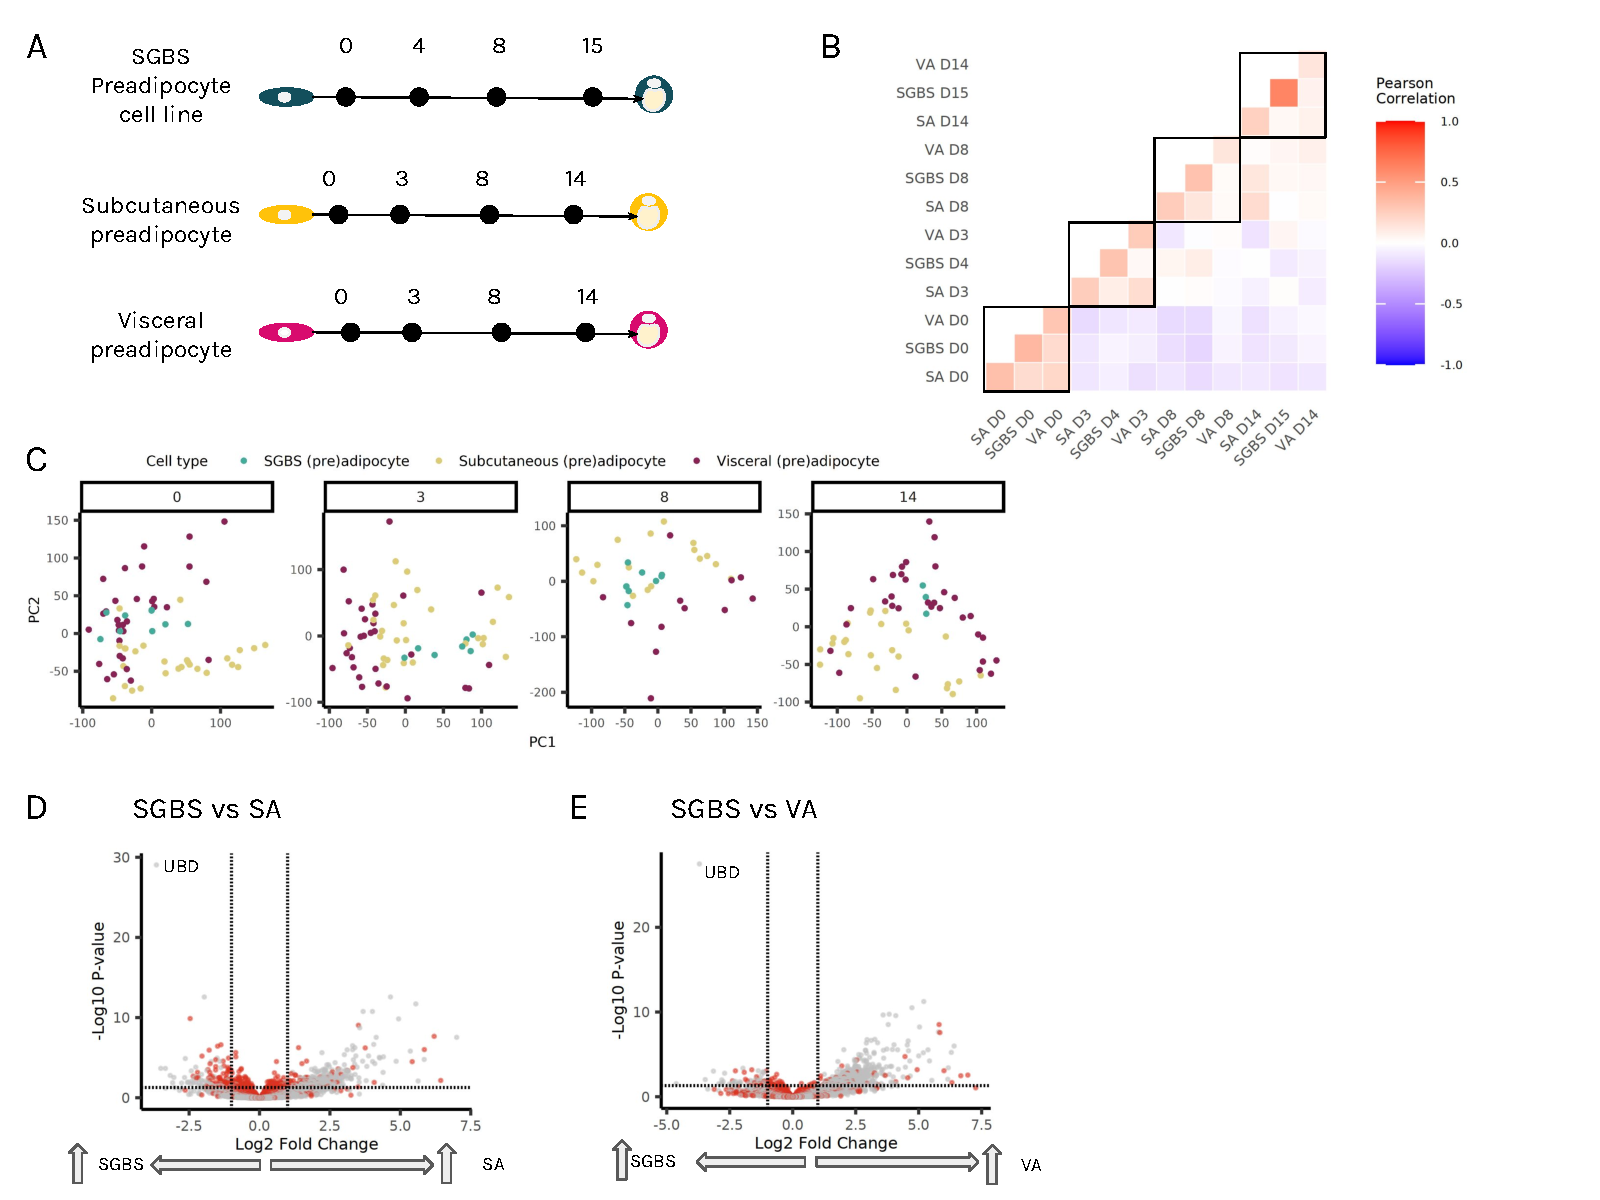
\includegraphics[width=\textwidth]{3_figures-and-files/Fig1.pdf}
    \caption[The transcriptional profiles of SGBS cells differ from both subcutaneous and visceral (pre)adipocytes.]{\textbf{The transcriptional profiles of SGBS cells differ from both subcutaneous and visceral (pre)adipocytes.} A. RNA-seq from 4 timepoints of differentiation was obtained for SGBS, subcutaneous, and visceral (pre)adipocytes. B. Pearson correlation applied on the PCs of each sample found more similarity by timepoint (black boxes) than the original source (VA, SA, SGBS). 
    C. PC 1 by PC 2 performed for each differentiation timepoint. For simplicity, days 3 and 4 were grouped together, and days 14 and 15 were put together. The SGBS cells, in teal, are found between the (pre)adipocytes of subcutaneous (yellow) and visceral (magenta) origin. 
    D, E. Volcano plots of the differential expression analysis performed for each depot against SGBS with the linear mixed model, $\mathrm{y} \sim \mathrm{depot} + (1 | \mathrm{timepoint})$. The red dots indicate genes with average expression of $>$ 1 CPM across all samples.
    }\label{fig: SGBS, subcutaneous, and visceral (pre)adipocyte transcriptional profiles}
\end{figure}

\subsection{Predicting transcription factors (TFs) to distinguish between subcutaneous and visceral (pre)adipocytes}

There are many existing methods to determine the TFs that define a cell type, ranging from purely computational to data-driven and validated\cite{Xu2021-bn,Joung2023-ft,Ng2021-kl,Ieda2010-rc,Stone2019-oe,Treutlein2016-hs}. Unfortunately, not all the databases include adipocytes or distinguish between types of adipocytes. Moreover, the methods that do have limited input samples for comparison between visceral and subcutaneous (pre)adipocytes. Thus, we applied the relevant ones to our question, and we complemented the results with our own analysis with a larger cohort of data.   

Mogrify predicts TFs for cell conversion by identifying those that are not only differentially expressed but also exert strong regulatory influence on other DEGs within a network\cite{Rackham2016-ef}. We ran the model to predict TFs to reprogram (pre)adipocytes between subcutaneous and visceral origins (\textbf{Figure 3.2A}). Intriguingly, the predicted TFs for the preadipocytes are not the same for the adipocytes. Moreover, KLF4 is both in the set for SPA to VPA and for VA to SA. The limited sample number (n=3 per celltype) from the FANTOM5 database is a caveat to these predictions.   

Another existing reference was built by D'Alessio and colleagues, which identifies candidate TFs using the Human Body Index collection\cite{D-Alessio2015-ia}. This algorithm evaluates the expression of each TF in the cell type of interest against the background of other cell types to determine candidate core TFs with high specificity to the cell type of interest. In this case, subcutaneous and visceral adipocytes are not being directly compared, but the TFs should reprogram a stem cell or fibroblast to SA or VA (\textbf{Figure 3.2A}). There are three redundant factors for the two cell types, PPARG, EBF1, and ZNF117, which would suggest that these three TFs are common for all adipocytes. While PPARG and CEBPA are required for differentiation from preadipocytes to adipocytes\cite{Lefterova2008-rk}, CEBPA is presented as a TF to reprogram a stem cell to a visceral adipocyte, which contradicts the Mogrify prediction that it would convert VA to SA. Collectively, Mogrify and D'Alessio models yield 46 TFs for depot-specific (pre)adipocyte reprogramming, accounting for overlaps and discrepancies between the models.

To further investigate these factors, we leveraged two independent cohorts of data from human subcutaneous and visceral (pre)adipocytes across differentiation\cite{Laber2023-qe,Bradford2019-ps}. Differential analysis was performed per timepoint and across four timepoints with a linear mixed model. Gene enrichment analysis and motif enrichment were applied to the DEGs to identify TFs that distinguish between the two depots. 38 of the 46 TFs are represented in the GSEA C3 Transcription Factor Targets Gene Set\cite{Liberzon2015-uo}, the HOMER human promoter set from RefSeq\cite{Heinz2010-lw}, and JASPAR2020\cite{Fornes2020-uo} (\textbf{Figure 3.2B}). The remaining 8 proposed TFs, DMRT2, ZNF117, PRICKLE1, SIK1, TXNIP, ARNTL2, IGF1, TSHZ2, should be tested experimentally.

\clearpage
\begin{figure}[!t]
    \centering
    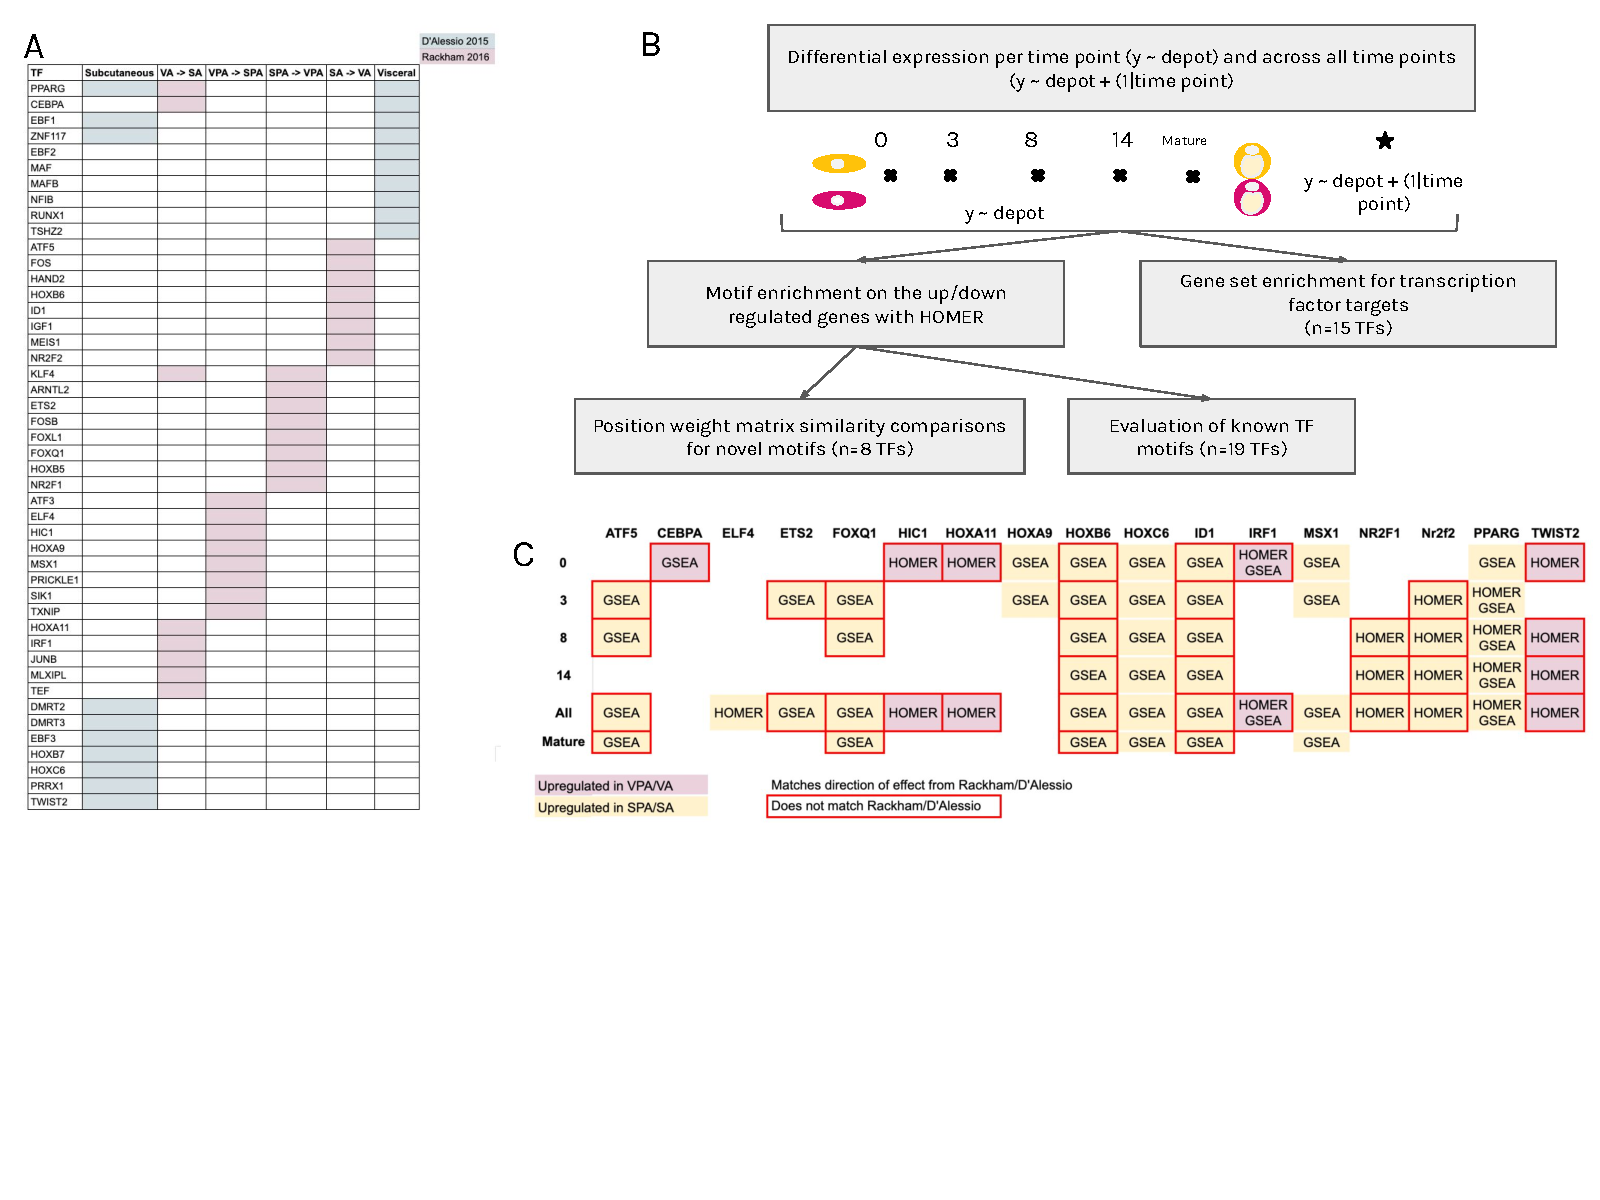
\includegraphics[width=\textwidth]{3_figures-and-files/Fig2.pdf}
    \caption[Candidate TFs predicted to distinguish between subcutaneous and visceral (pre)adipocytes include PPARG as a factor that is upregulated in subcutaneous (pre)adipocytes.]{\textbf{Candidate TFs predicted to distinguish between subcutaneous and visceral (pre)adipocytes include PPARG as a factor that is upregulated in subcutaneous (pre)adipocytes.} 
    A. The 46 TFs that are predicted to reprogram (pre)adipocytes from established methods. The colors indicate the data source. B. Workflow to evaluate the predicted TFs in two independent datasets\cite{Laber2023-qe,Bradford2019-ps}. Differential expression was performed for each timepoint and across all timepoints, and the results were put through motif enrichment and gene set enrichment analysis. C. Summary of the results from HOMER and GSEA, organized by differential expression model timepoint (row) and TF (column), colored by upregulation in subcutaneous (pre)adipocytes (yellow) or visceral (pre)adipocytes (pink). 5 TFs replicated in the same direction of effect, while 12 TFs were found in the opposite direction than predicted in A (red outline). 
    }\label{fig: Candidate TFs for depot specific reprogramming}
\end{figure}

17 of the predicted TFs were significantly enriched for either depot in at least one differential expression model across the TF identification methods (\textbf{Figure 3.2C}). The directional activity of each TF was internally consistent across the six models, with motif and gene set enrichment analyses identifying the same upregulated depot in every instance of overlapping detection. With the exception of ELF4, all the other TFs had significantly enriched activity in more than one model. Only 5 of these were concordant with the directionalities of the candidate reprogramming factors: ELF4, HOXA9, HOXC6, MSX1, and PPARG. PPARG was consistently enriched for subcutaneous (pre)adipocytes across five models and both gene set and motif enrichment analyses. 

D'Alessio predicted CEBPA as a factor for VA, which is supported by upregulated CEBPA activity in Day 0 visceral preadipocytes, but Mogrify identified CEBPA as a TF to convert VA to SA. HIC1, HOXA11, IRF1, and TWIST2 were predicted to identify subcutaneous (pre)adipocytes, but they are upregulated in visceral (pre)adipocytes. On the other hand, ATF5, ETS2, FOXQ1, HOXB6, ID1, NR2F1, and NR2F2 are all more active in subcutaneous (pre)adipocytes, despite initial predictions for visceral (pre)adipocyte fate. While gene expression does not necessarily correlate with transcription factor activity level\cite{Cheng2007-mc}, NR2F1 is more highly expressed in human visceral adipocytes\cite{Gesta2006-so}, which supports the Mogrify prediction. RUNX1 was nominally more active in visceral Day 3 preadipocytes than subcutaneous (p=0.01; q=0.0646), which is the predicted direction of effect from D'Alessio, but it was not found to be significantly enriched in visceral (pre)adipocytes. Overall, the minimal reproducibility of the TFs across the various methods highlights the need for more data. These results can be used to prioritize factors for testing, but all 46 proposed TFs should be evaluated for reprogramming.

\subsection{Developing a method to evaluate the reprogrammed cells}

After modification of SGBS cells with the proposed TFs, a robust analytical protocol is required to evaluate the reprogrammed state. To quantify reprogramming success, the transcriptomes of reprogrammed and thus unknown “query” cells will be captured via snRNA-seq and systematically benchmarked against reference profiles of both the original SGBS and target SA/VA cell types. We tested an assortment of computational conditions, including varying feature selection and integration methods, using two recent adipocyte snRNA datasets\cite{Emont2022-pb,Lazarescu2025-ru}. One limitation of sc/snRNA-seq is sparse data, in that there are many genes with zero counts, which can be biological, technical, or sampling in origin\cite{Jiang2022-yf}. To circumvent the sparse data and increase the reliability of results, pseudobulks can be generated for sc/snRNA-seq\cite{Squair2021-wz}. A pseudobulk is an aggregated transcriptional profile from a group of cells with the same label or cell type. It increases the stability of methods applied to sc/snRNA-seq data, such as differential expression or cell type classification\cite{Squair2021-wz,Adamson2016-gi}.   

\clearpage
\begin{figure}[!t]
    \centering
    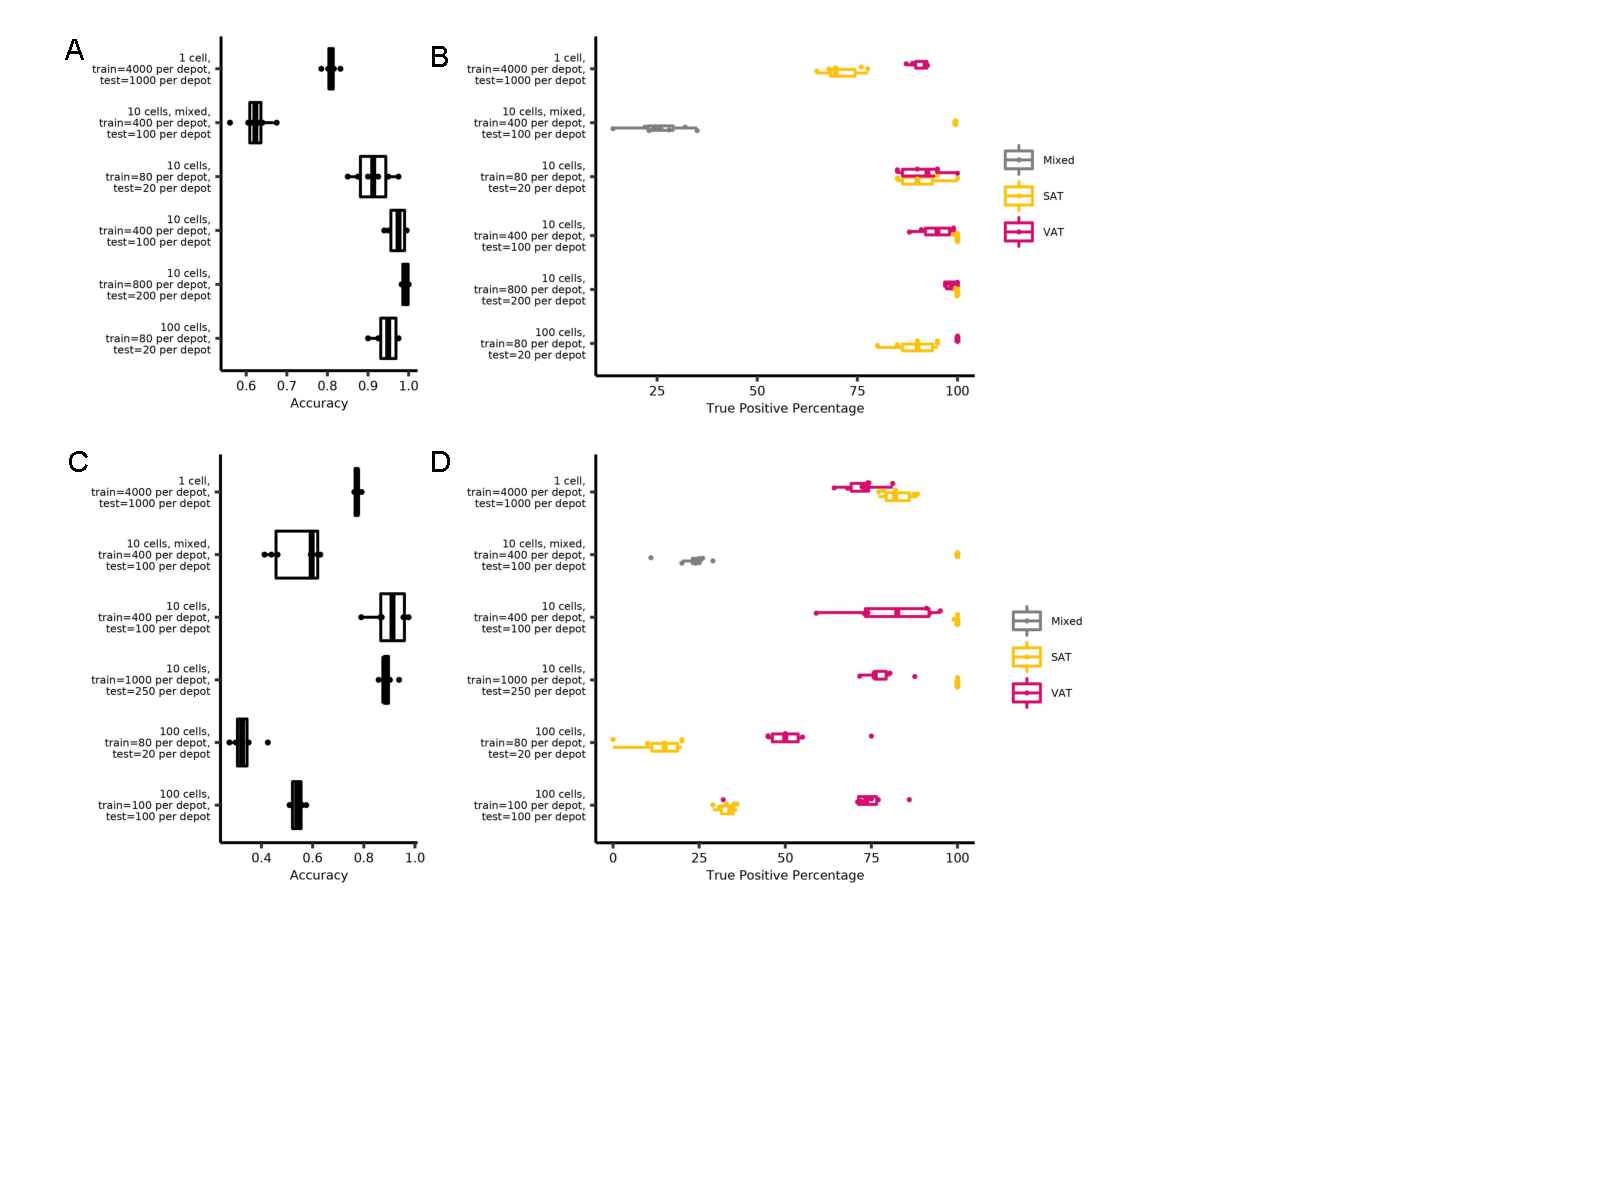
\includegraphics[width=\textwidth]{3_figures-and-files/Fig3.pdf}
    \caption[Pseudobulks of 10-cells with large training sets have high accuracy for predicting cell identity between subcutaneous and visceral adipocytes.]{\textbf{Pseudobulks of 10-cells with large training sets have high accuracy for predicting cell identity between subcutaneous and visceral adipocytes.} 
    A. Accuracy of Capybara models on Emont adipocytes. B. Percent of true positive results in the Emont models, separated by cell identity. C. Accuracy of Capybara models, trained on Emont data, tested on Lazarescu adipocytes. D. Percent of true positive results in the Lazarescu models, separated by cell identity. 
    }\label{fig: Evaluating cell identify with single cell RNAseq and pseudobulking}
\end{figure}

Capybara is an unsupervised computational method that scores cells against references using quadratic programming and has the framework to allow for multiple identities, including “multi” and “unknown”, enabling the identification of hybrid cells during reprogramming\cite{Kong2022-pg}. Capybara was run on the human adipocyte samples from Emont et al., using the single-cell data , pseudobulks generated from groups of 10 cells, and pseudobulks of 100 cells. A mixed population containing both visceral and subcutaneous adipocytes was also generated for the 10-cell pseudobulks to assess the multiple identity capacity within Capybara. With the single-cell data, the depot was correctly assigned with accuracy of 0.809$\pm$0.016, and the accuracy increased with pseudobulks (\textbf{Figure 3.3A}). Within the 10-cell pseudobulk, accuracy correlated with sample depth, from 0.972+0.023 with 500 pseudobulks per depot to 0.992+0.008 with 1,000 samples per depot. At the same sample depth of 100 samples, the 100-cell pseudobulks model (0.946+0.029) had higher accuracy than the 10-cell pseudobulk model (0.876+0.039). This indicates that the accuracy and precision of the predictions could be even greater with more samples. The results are bolstered by the mixed depot 10-cell pseudobulks, which had the lowest accuracy (0.633+0.024) and faithfully identified that there were mixed samples, detecting 25.5\% of the mixed pseudobulks (\textbf{Figure 3.3B}). Unexpectedly, the true positive rates of each depot varied between conditions. Subcutaneous adipocytes had a lower true positive percentage (70.9$\pm$1.99) in the single-cell and 100-cell pseudobulk models compared to visceral adipocytes (90.8$\pm$0.918), while the opposite trend held for most of the 10-cell pseudobulks (\textbf{Figure 3.3B}). This could be attributed to missing or lowly expressed genes that contribute significantly to cell identity. 

To increase sample number and test how the models work across datasets, the Emont-integrated transcriptomes from the Lazarescu et al. adipocytes were pseudobulked and classified (\textbf{Figure 3.3C, D}). The 10-cell pseudobulk model outperformed both the single-cell and 100-cell approaches, achieving accuracies of 0.903$\pm$0.073 and 0.890$\pm$0.027 across two sample depths. In comparison, the single-cell model reached an accuracy of 0.774$\pm$0.011, and the 100-cell pseudobulk 0.333$\pm$0.0517, at the same split ratio. While increasing the sample depth with an adjusted split ratio improved the 100-cell model, its accuracy remained low (0.540$\pm$0.0251) due to insufficient input data. Both 100-cell models were surpassed by the depot 10-cell pseudobulk model in accuracy (0.547$\pm$0.092), further indicating that more samples are necessary when combining different sc/snRNA datasets, even with computational integration. Intriguingly, the true positive percentage for subcutaneous adipocytes still approached 100\% in the 10-cell pseudobulk methods, and the predictions for visceral adipocytes were less accurate. This suggests that the transcriptional signature of subcutaneous adipocytes is more robust than visceral adipocytes. Altogether, despite being trained and tested on different datasets, the 10-cell pseudobulk models predicted cell identity with $>$0.890 accuracy, which is highly promising for future applications.

\section{Discussion}

In this chapter, we set up the analytical framework for reprogramming depot-specific adipocytes. We explored whether SGBS cells would be suitable progenitors to model human (pre)adipocytes from both subcutaneous or visceral origin through transcriptomics. The TFs to convert precursors to SA and VA were evaluated using a series of curated methods, and models scoring the success of reprogramming were explored. This novel proposal is unique in its application of cell identity methods and pseudobulking on depot-specific adipocytes.   

The 46 candidate TFs we identified for subcutaneous and visceral (pre)adipocyte reprogramming are well supported in the literature. In this chapter, PPARG was consistently found across many time points and modalities as having upregulated activity in subcutaneous (pre)adipocytes. This aligns with previous data for mouse and human adipocytes: in human preadipocyte samples, visceral adipocytes have lower expression of adipogenic factors, including PPARG\cite{Mathur2022-fx}; in mouse cells, visceral preadipocytes cultured ex vivo require BMP-4 in addition to the standard differentiation cocktail to induce expression of Pparg and stimulate adipogenesis\cite{Macotela2012-wy}; and human SA have reduced methylation at \textit{PPARG} and its binding partner RXRa compared to VA\cite{Bradford2019-ps}. Moreover, familial partial lipodystrophy type 3 (FPLD3) is caused by pathogenic variants in PPARG\cite{Rutkowska2022-rs}. This rare genetic disorder results in a loss of subcutaneous fat from lower limbs without affecting visceral fat accumulation, highlighting the depot-specific activity of PPARG.

Additionally, 6 HOX TFs were predicted to induce depot-specificity, and the literature contains many examples of differentially expressed HOX genes between depots, although not all of our predictions are concordant with existing knowledge\cite{Ahn2019-us,Gesta2007-cp}. One that is consistent is HOXA9, which is more active in subcutaneous (pre)adipocytes and has been observed to be more highly expressed in SAT than VAT\cite{Tchkonia2007-xa}.  

Furthermore, a genome wide methylation study performed on SA and VA examined TF binding motifs within 150 base pairs of the methylated sites and identified 49 transcription factors that corresponded to 7 binding motifs in SA\cite{McAllan2023-qo}. 9 of these overlapped with our 46 of interest, including 5 that were intended for reprogramming into SA: ATF3, JUNB, KLF4, ELF4, and HOXA11. Lazarescu et al. also identified TFs of interest for depot-specificity using SCENIC, a method for regulatory network and cell identity clustering\cite{Aibar2017-wj}. They found one regulon that is different between visceral and subcutaneous adipocytes, containing CEBPA, which was enriched in VA but not SA, as well as RUNX1. This is concordant with the D'Alessio predictions and the gene set enrichment results. The genes enriched for subcutaneous adipocytes were STAT4 and RELA, which were not in our set of 46\cite{Lazarescu2025-ru}. In addition, lineage tracing studies have identified Prx1 as a selective marker for subcutaneous adipocytes and Wt1 for visceral preadipocytes\cite{Sakers2022-wb}. Collectively, these studies suggest a broader landscape of candidate TFs for (pre)adipocyte reprogramming.  

The significance of this work would include not only the computational methods but also the physical resource of depot-specific (pre)adipocytes to enable further research. Visceral adipocytes contribute to ovarian cancer metastasis\cite{Nieman2011-hq} and are associated with ovarian cancer chemoresistance\cite{Lin2024-ov}. The study that identified the chemoresistance correlation used a 3-cell coculture model, in which the adipocytes were either primary culture omental adipocytes or differentiated 3T3-L1 cells, which are a mouse preadipocyte cell line. The objective of this work would be to enable future investigators to use a human visceral adipocyte cell line instead of the mouse fibroblast. Furthermore, there was internal consistency in the TF predictions, but many of the candidate 46 were not uncovered by the enrichment analyses. This could be indicative of differences between initial data sources, especially with the caveats that the subcutaneous and visceral (pre)adipocyte transcriptomic data is derived from cells differentiated ex vivo\cite{Laber2023-qe}, while the Mogrify model had three replicates per cell type\cite{Rackham2016-ef}. This highlights the need to reprogram depot-specific adipocytes to enable future comparisons. The factors identified could be applied to cell types other than SGBS cells, such as stem cells and induced pluripotent stem cells, such that the effects of genetic mutations on visceral versus subcutaneous adipocytes could be robustly compared.  

While this framework provides a theoretical blueprint for depot-specific reprogramming, several limitations remain. The current reliance on transcriptomic data provides a high-resolution snapshot of cell state, but lacks the epigenetic context required to fully map the regulatory landscape. Future iterations of this model would benefit from the integration of ATACseq data to further refine the candidate set of 46 factors\cite{Halasz2023-xu,Lee2024-ix}. Furthermore, while our pseudobulking approach successfully prevented data leakage and ensured internal consistency, the resulting data bottleneck for the 100-cell models suggests that future studies utilize even larger datasets to improve model generalizability. Ultimately, the transition from this computational framework to in vitro experimental validation will be the definitive test of these predicted TFs. Several critical parameters remain to be optimized, including the number of TFs delivered simultaneously, the activation method (e.g., viral overexpression or CRISPRa), and the specific “dosage” of each factor. Because many identified TFs exhibit activity in both subcutaneous and visceral depots, achieving the precise threshold of upregulation necessary to drive a depot-specific identity is essential. Addressing these pending questions will move us closer to generating subcutaneous and visceral (pre)adipocyte cell lines.   

This work establishes a novel analytical framework for the depot-specific reprogramming of human adipocytes, utilizing SGBS cells as a versatile progenitor model. By integrating multiple transcriptomic datasets and literature-backed methods, we generated a candidate set of 46 transcription factors to identify key regulators of depot identity, such as PPARG and members of the HOX family. We further applied pseudobulking without replacement to a cell identification method to create high-fidelity models for scoring adipocyte reprogramming and demonstrated that 10-cell pseudobulks provide optimal predictive accuracy. This research provides a theoretical foundation for creating human subcutaneous and visceral (pre)adipocytes from the same original cell line, offering a more physiologically relevant alternative for studying adipocytes and adipocyte-driven pathologies.

%%%%%%%%%%%%%%%%%%%%%%%%%%%%%%%%%%%%%%%%%%%%%%%%%%%%%%%%%%%%%%%%%%%%%%%%%%%%%%%%
\section{Methods}
%%%%%%%%%%%%%%%%%%%%%%%%%%%%%%%%%%%%%%%%%%%%%%%%%%%%%%%%%%%%%%%%%%%%%%%%%%%%%%%%

\subsection{Analysis of bulk RNA-seq datasets}

We analyzed the bulk RNA-seq datasets of human derived subcutaneous and visceral adipocytes (GSE184089 and GSE110821) and SGBS cells (GSE274839, GSE245619, and GSE262480). Raw sequencing reads were aligned to the reference hg38 using Kallisto with default parameters\cite{Bray2016-zt} to generate gene counts per sample. Analysis was performed in R 4.1.3.   

In GSE184089, adipose derived mesenchymal stem cells (AMSCs) were sequenced at four timepoints of adipocyte differentiation, from early preadipocytes to full adipocytes. 2 outliers were removed, and 3 samples were relabeled after initial processing indicated they were mislabeled.

\subsubsection{Visualizing the transcriptional profiles of SGBS, subcutaneous, and visceral (pre)adipocytes}
ComBat-seq was run between datasets (GSE274839, GSE245619, GSE262480, and GSE184089) for batch correction\cite{Zhang2020-kq}. The smallest group was the Day 15 SGBS samples (n=3), and the largest were the visceral Day 0 preadipocytes and visceral Day 14 adipocytes (n=32). EdgeR 3.36.0 and limma-voom (limma v3.50.1) were used to filter and normalize reads for library size\cite{Robinson2010-qx,Law2014-yh}. 28,757 genes were retained across 234 samples. PCA was performed with prcomp() across all samples and by time point. The correlation plot was generated from the cor() on the PCA results of the full dataset, taking the average per cell type and time point. 

\subsubsection{Differential expression between SGBS, subcutaneous, and visceral (pre)adipocytes}
ComBat-seq was run between datasets (GSE274839 and GSE184089) for batch correction\cite{Zhang2020-kq}. EdgeR 3.36.0 and limma-voom (limma v3.50.1) were used to filter and normalize reads for library size\cite{Robinson2010-qx,Law2014-yh}, retaining 27,134 genes and 218 samples. Differential expression was performed for each depot (subcutaneous and visceral) against SGBS in dream\cite{Hoffman2021-xx} using a linear mixed model with gene expression as a result of fixed effect depot and random effect differentiation day, $\mathrm{y} \sim \mathrm{depot} + (1 | \mathrm{day})$.

\subsection{Identifying candidate transcription factors}
Mogrify and the atlas built by D'Alessio were used as directed by the manuscripts\cite{Rackham2016-ef,D-Alessio2015-ia}. For Mogrify, each TF is ranked based on a weighted sum of its regulatory influence, and the optimal set of TFs is selected to account for 98\% of regulatory coverage \cite{Rackham2016-ef}. Its database has n=3 for each SPA, VPA, SA, and VA.

\subsubsection{Differential expression between subcutaneous and visceral (pre)adipocytes}
EdgeR 3.36.0 and limma-voom (limma v3.50.1) were used on GSE184089 to filter and normalize reads for library size\cite{Robinson2010-qx,Law2014-yh}, retaining 24,269 genes and 206 samples. A cell-means linear model, in which samples were categorized into eight discrete groups representing each depot-time combination (SA and VA; Days 0, 3, 8, and 14), was performed in dream\cite{Hoffman2021-xx}, and contrasts were calculated between each depot for every time point. In addition, a linear mixed model with gene expression as a result of fixed effect depot and random effect differentiation day, $\mathrm{y} \sim \mathrm{depot} + (1 | \mathrm{day})$. For the mature adipocytes, edgeR 3.36.0 and limma-voom (limma v3.50.1) were used on GSE110821 to filter and normalize reads for library size, retaining 13,1472 genes and 6 samples, and perform differential expression analysis by depot\cite{Robinson2010-qx,Law2014-yh}.

\subsubsection{TF identification}
TF Gene set enrichment was run with fgsea v1.20.0\cite{Korotkevich2021-ra} on the transcription factor pathways in Gene Ontology C3 transcription factor targets (TFT) using the parameters minSize=10, maxSize \= 1500, and nPermSimple=10000\cite{Subramanian2005-bj,Mootha2003-ys}. FindMotifs was run in HOMER with the parameters \-start \-1000 \-end 1000\. 8 TFs have known motifs in JASPAR but are not present in either the GO C3 TFT collection or the HOMER Refseq promoter set. These genes are PRRX1, DMRT3, EBF3, FOSB, HOXB5, NFIB, MLXIPL, and FOXL1. To determine if any of these TFs were enriched, the position weight matrices (PWMs) for these transcription factors were scored against the top novel HOMER results. There were no Pearson correlations greater than 0.7, indicating that none of the novel motifs align with the motifs of these 8 TFs.  

\subsubsection{Processing adipocyte sc/snRNA-seq}
Human adipocyte snRNA-seq was downloaded in rds format from the Emont lab\cite{Emont2022-pb}. Analysis was performed in R 4.3.1 with Seurat 4.3.0.1. The adipocytes were subset into two objects by depot (11,475 visceral adipocytes and 14,396 subcutaneous adipocytes), and a sparse matrix of the raw counts from each object was exported. Pseudobulks without replacement were generated in 10 and 100-cell iterations. Mixed 10-cell pseudobulks were created with commonly expressed genes and equal proportions of VA and SA cells (n=2,294).  

The snRNA-seq of human subcutaneous and visceral adipocytes, integrated with Emont et al., were downloaded from CZ CELLxGENE\cite{Lazarescu2025-ru,CZI-Cell-Science-Program2025-eh}. Analysis was performed in R 4.3.1 with Seurat 4.3.0.1 after the h5ad file was converted into a Seurat Object. There were 26,601 subcutaneous adipocytes and 26,935 visceral adipocytes. Pseudobulks were generated as described above. 

\subsection{Implementing Capybara}
The cell identification method was applied following the original protocol \newline https://github.com/morris-lab/Capybara with a few modifications\cite{Kong2022-pg}. For each iteration, the snRNA sparse matrices were randomly subset and formatted to match the Capybara reference and test matrices. There were an equal number of SA and VA (or SA and mixed) samples for each test dataset and train dataset. A high-resolution reference was constructed from the reference matrix and metadata, and quadratic programming was performed on the reference and subsequently on the test. Cell types were then classified and scored. For each condition, n=6 for SA vs VA, and n=8 for SA vs mixed.

\subsection{Proposed experimental outline}
We will use CRISPR activation (CRISPRa) to overexpress our TFs of interest in SGBS cells. The advantages of this model over other forms of induced overexpression are the high multiplexing capacity and direct transcriptional activation from endogenous loci activation \cite{Sokka2022-ax}. There have been CRISPRa reprogramming screens \cite{Yang2019-wd,Liu2018-fc}, and targeted CRISPRa for the reprogramming of lymphoblastoid cell lines to induced pluripotent cells showed high fidelity and homogeneity, indicating it can be more successful than conventional methods \cite{Sokka2022-ax}.   

SGBS cells will be transduced with a doxycycline-inducible dCas9-VPR to generate a CRISPRa cell line. The 46 transcription factors identified will be activated singly and in pairwise combinations using CROPseq-multi\cite{Walton2024-xj}. A library of constructs consisting of single and dual guide RNAs (sgRNAs) corresponding to each of the TFs, with two independent sgRNAs per TF, and 20\% non-targeting control (NTC) sgRNAs, will be constructed. The sgRNAs will be identified through CRISPick, which optimizes differently for CRISPRa/i guides\cite{Sanson2018-bh,Doench2016-bp}. Chromosomal positioning of the sgRNAs will also be taken into account to optimize the binding of many activators to the promoter region.   

This library will be transduced at MOI=0.15 into the dCas9-VPR inducible SGBS adipocytes such that each perturbation is replicated in 1000 cells. After 7 days, the transduced SGBS cells will be subjected to scRNA-seq using the 10x Genomics platform as detailed in the preliminary data to generate a per cell transcriptomic profile. Notably, the sgRNA vector design enables for each cell identification of the sgRNAs transduced as well activation of the target TF. Thus only cells with successfully induced activation will be retained for analysis\cite{Walton2024-xj}.   

As alternatives, we will also explore transgenes and multiplexed open reading frames, in case the CRISPRa SGBS cell line is not viable\cite{Joung2023-ft}.

% References
\bibliographystyle{unsrtnat}
\bibliography{bib_3.bib}
\begin{dissertationepilogue}

    % Fix a bug in the numbering of the epilogue chapters?
    \setcounter{chapter}{4}
    \setcounter{section}{0}

    \section{Conclusion}
    Insulin resistance (IR) is a global epidemic, and it is imperative to shift from broad-spectrum pharmacology toward precision molecular targeting to combat this multifaceted condition. While the therapeutic potential of PPAR$\gamma$ has been recognized for decades, the clinical utility of thiazolidinediones (TZDs) remains constrained by their adverse side-effect profile\cite{Yki-Jarvinen2004-bc}. As a master regulator of adipocyte differentiation, PPAR$\gamma$ orchestrates the development and maintenance of adipose tissue\cite{Tontonoz2008-pe} and contributes to distinctions between adipose depots: adipocytes derived from visceral adipose tissue, which is associated with exacerbating the pathogenesis of IR-related diseases\cite{Preis2010-eh,Agrawal2023-ee}, exhibit reduced PPARG activity compared to subcutaneous adipocytes\cite{Bradford2019-ps,Mathur2022-fx}. Despite these insights, the molecular mechanisms by which depot specific adipocytes affect adipose tissue dysfunction and systemic insulin resistance remain poorly defined\cite{Sebo2019-nh,Sakers2022-wb}. This dissertation addressed these challenges by integrating functional genomics with human genetics to uncover a novel translational start site within PPARG and by developing a computational infrastructure to generate and interrogate depot-specific adipocytes.

    
    %%%%%%%%%%%%%%%%%%%%%%%%%%%%%%%%%%%%%%%%%%%%%%%%%%%%%%%%%%%%%%%%%%%%%%%%%%%%
    \section{Summary}
    %%%%%%%%%%%%%%%%%%%%%%%%%%%%%%%%%%%%%%%%%%%%%%%%%%%%%%%%%%%%%%%%%%%%%%%%%%%%

    In Chapter 1, we investigate the coding landscape of PPARG and identify an alternative translational start site at methionine 135. This discovery redefines our understanding of the PPARG locus, demonstrating that the upstream region encoding the activation-function 1 (AF-1) domain of the protein is not necessary for function. The novel translational initiation site generates the isoform PPAR$\gamma$ M135, which manifests superior transactivation of target genes than the canonical PPAR$\gamma$2 isoform in response to TZD treatment.
    
    The therapeutic relevance of PPAR$\gamma$ M135 was confirmed in Chapter 2 through a combination of in vitro modeling and human genetic association studies. SGBS human adipocytes engineered to express PPAR$\gamma$ M135 exhibited increased insulin-sensitizing capacity relative to wild-type controls. Consistent with the heightened activity of this truncated isoform, human genetic variants that attenuate the PPARG AF-1 domain correlate with favorable metabolic profiles, as quantified by a metabolic syndrome severity score (METSS) developed within this study. Together, these findings suggest that AF-1 inhibition or selective expression of PPAR$\gamma$ M135 may amplify the therapeutic benefits of PPAR$\gamma$ agonism while minimizing the adverse effects associated with conventional TZDs.
    
    Finally, in Chapter 3, we provide a framework for modeling depot-specific adipocytes. SGBS cells were verified as a suitable progenitor model for both visceral and subcutaneous adipocytes, though other multipotent stem cells or fibroblasts may offer similar utility. We identified 46 candidate transcription factors (TFs) that distinguish between subcutaneous and visceral (pre)adipocytes and applied orthogonal methods to substantiate 17 TFs, including PPARG. To evaluate the reprogrammed cells, we proposed a computational blueprint that implemented cell identity scoring methods on pseudobulked single cell RNAseq and achieved high accuracy. This work provides a foundation to further study the mechanisms contributing to IR in the cellular contexts in which they manifest.

    %%%%%%%%%%%%%%%%%%%%%%%%%%%%%%%%%%%%%%%%%%%%%%%%%%%%%%%%%%%%%%%%%%%%%%%%%%%%
    \section{Limitations and Future Directions}
    %%%%%%%%%%%%%%%%%%%%%%%%%%%%%%%%%%%%%%%%%%%%%%%%%%%%%%%%%%%%%%%%%%%%%%%%%%%%

    The PPAR$\gamma$ M135 isoform demonstrates that extensively studied genes still harbor critical, undiscovered regulatory mechanisms with profound clinical implications. The plethora of data generated from single cell functional genomics methods could be helpful in this pursuit.
    
    One innovation in this thesis was the development of the metabolic syndrome severity score (METSS), which assessed metabolic syndrome in the UK Biobank based on five clinical components. However, this score had limited application and scope, as the clinical landscape progresses quickly, especially with multifaceted conditions. This was recently exemplified by the evolution of steatotic liver disease nomenclature. In 2021, I wrote a review about the human genetics underlying non-alcoholic fatty liver disease (NAFLD), in which I discussed the difficulties of diagnosing and classifying NAFLD and annotated each known genetic variant by the specific phenotypes it was found to be associated with, such as histologically defined steatosis, liver fat measured by imaging modalities, and liver enzyme levels\cite{Du2021-bq}. In the review process, we were asked to include a section addressing metabolic dysfunction-associated fatty liver disease (MAFLD), a new name and set of diagnosis criteria proposed by experts in the field in 2020\cite{Eslam2020-ud}. In 2023, another name and definition were introduced: metabolic dysfunction-associated steatotic liver disease (MASLD)\cite{Rinella2023-oe}. While the two new terms are still under debate\cite{Ramirez-Mejia2024-jo}, in just two years, the review I wrote became obsolete. I strongly support this trajectory toward precision medicine, as both MAFLD and MASLD are examples of reducing ambiguity, removing stigma from medical terms, and replacing invasive diagnostic methods with minimally invasive measurements, all of which benefit patients, researchers, and clinicians. Similarly, for metabolic syndrome, we are moving from using binary definitions\cite{Kraja2011-ja}, to severity indices\cite{Gurka2014-ib}, to multivariate genomic analysis\cite{Park2024-da}. While METSS served as a robust tool for this specific study, future applications will have better methods that reflect our deepening understanding of metabolic health.
    
    The reprogramming framework proposed in Chapter 3 offers significant potential for expanding our understanding of adipocytes and mechanisms underlying IR beyond the current models. However, translating this computational framework into a viable experimental system presents substantial technical hurdles. The multifactorial nature of cellular reprogramming requires rigorous optimization of experimental conditions to evaluate candidate transcription factors (TFs), adipocytes are particularly difficult to work with due to cellular fragility, and many TFs were proposed. More adipocyte and adipose tissue datasets would be beneficial. Ideally, the proposed framework could also be extended to model other understudied cell types with primarily transcriptomic data.
    
    During my PhD, I used functional genomics combined with human genetics to determine causal mechanisms of insulin resistance, with a focus on key regulators and cell types in adipose tissue.  Looking forward, the field should prioritize high-resolution, multimodal research on adipocyte biology to further elucidate the mechanisms driving insulin resistance. 

\end{dissertationepilogue}

\bibliographystyle{unsrtnat}
\bibliography{bib_4.bib}

%%%%%%%%%%%%%%%%%%%%%%%%%%%%%%%%%%%%%%%%%%%%%%%%%%%%%%%%%%%%%%%%%%%%%%%%%%%%%%%%
% Appendix of the Dissertation
%%%%%%%%%%%%%%%%%%%%%%%%%%%%%%%%%%%%%%%%%%%%%%%%%%%%%%%%%%%%%%%%%%%%%%%%%%%%%%%%
\appendix

\appendix{}

\chapter{Supplemental Material for Chapter \ref{chap:chapter 1}}

Additional supplemental material can be found in the published location at \url{https://doi.org/10.2337/db24-0497}. 

\begin{figure}[h]
    \centering
    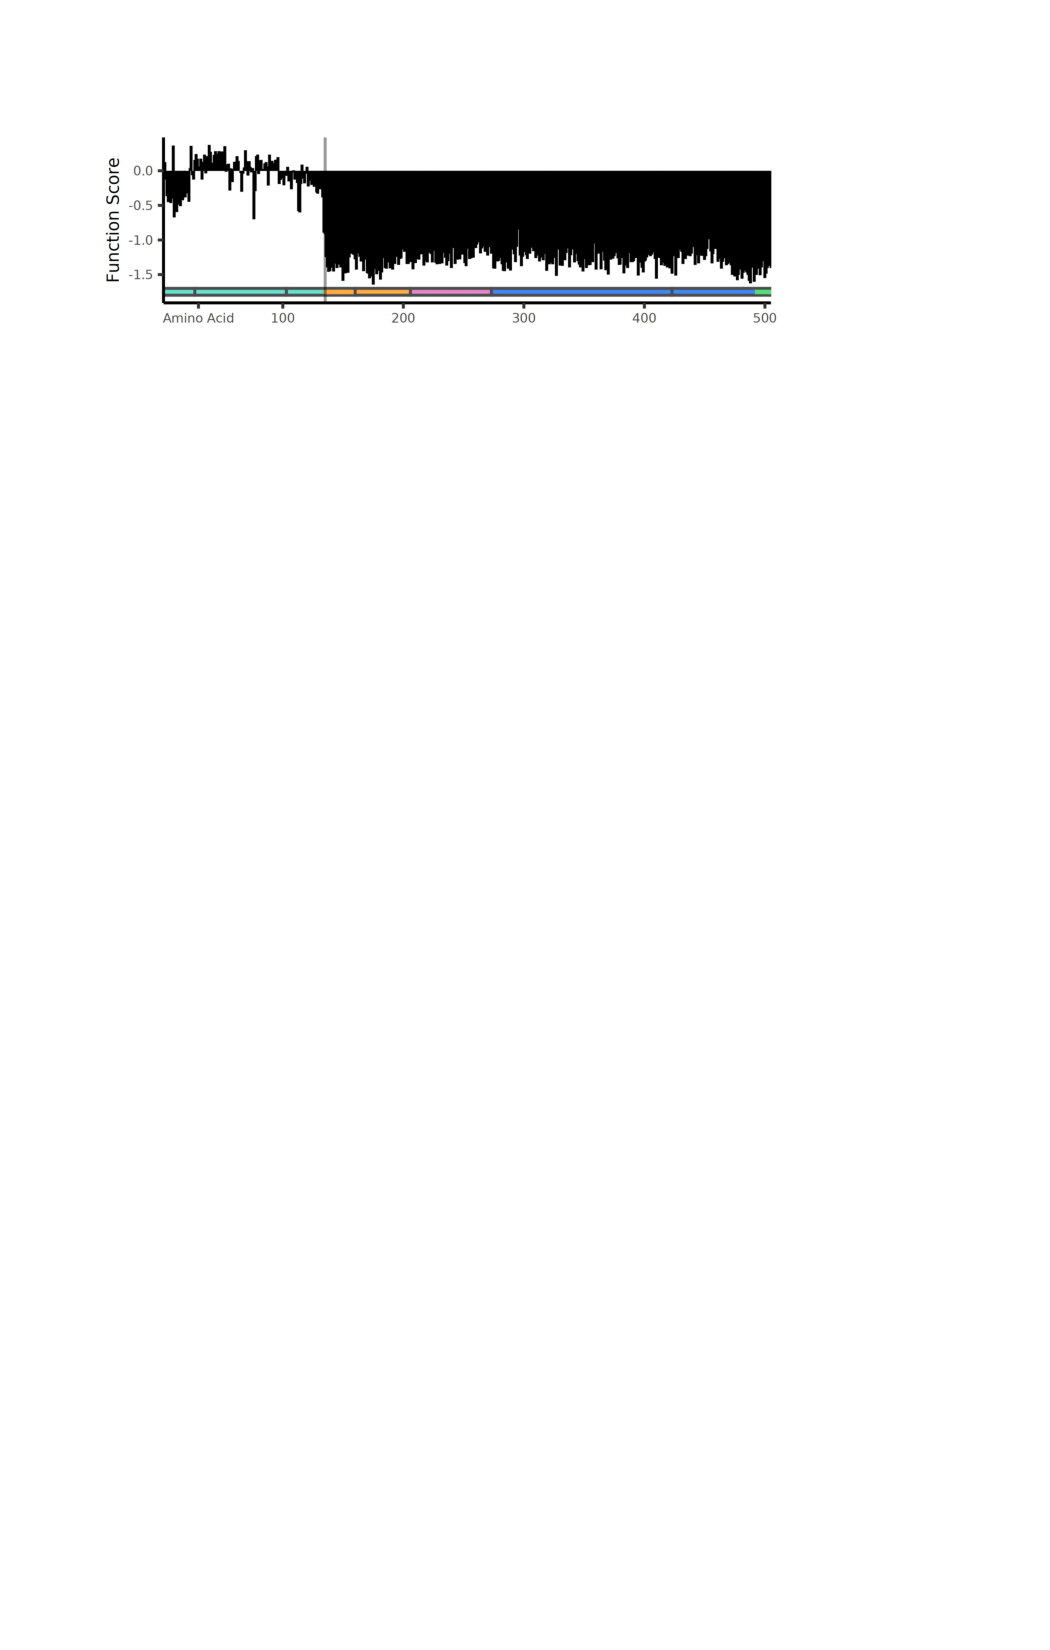
\includegraphics[width=\textwidth]{1_figures-and-files/FigS1.pdf}
    \caption[Alternative start site present with endogenous ligand.]{\textbf{Alternative start site present with endogenous ligand.} Function scores (FS) of insertions/deletions (indels) at each amino acid of PPAR$\gamma$2 calculated as previously published (Majithia et al. 2016) after 10 $\mu$M prostaglandin J2 (PGJ2) treatment. This response to an endogenous ligand is similar to the effect induced by the synthetic drug, rosiglitazone (\textbf{Figure 1.1D}). FS=0 refers to wild-type activity. 
    }
\end{figure}


\clearpage
\begin{table}[h]
  \centering
  \caption[CRISPR guides and genotypes from the monoclonal cell lines.]{\textbf{CRISPR guides and genotypes from the monoclonal cell lines.} Cell lines with guides targeted to \(PPARG\) intronic sequence (Int-sgRNA), to be used as control, targeted to exon 1 (Ex1-sgRNA), for pre-p.M135 edits, and targeted to exon 3 (Ex3-sgRNA), for post-p.M135 edits.
  }
\begin{tabular}{|c|c|c|m{4.7cm}|m{2.8cm}|}
    \hline
    Guide Name & Cut Site (hg38) & Zygosity & Genotype & Protein\newline Consequence \\
    \hline
    Int-sgRNA & chr3:12363492 & +/+ & WT & PPAR$\gamma$ \\
    \hline
    \multirow{4}{*}{Ex1-sgRNA} & \multirow{4}{*}{chr3:12379745} & \multirow{2}{*}{+/-} & chr3:12379749\_12379751delo\newline 12379744\_12379750del & p.N42GfsX50 \\
    \cline{4-5}
                                &                               &                       & chr3:12379736\_12379744delo\newline 12379741\_12379751del & p.T41SfsX48 \\
    \cline{3-5}
                                &                               & \multirow{2}{*}{-/-} & chr3:12379744\_12379973del & p.PPAR$\gamma\Delta$1 (deletion exon 1) \\
    \cline{4-5}
                               &                               &                       & chr3:12379702\_12379773del & p.PPAR$\gamma\Delta$1 (deletion exon 1) \\
    \cline{3-5}                                                        
    \hline
    \multirow{2}{*}{Ex3-sgRNA} & \multirow{2}{*}{chr3:12392733} & \multirow{2}{*}{-/-} & chr3:12392733insA & p.V201SfsX206 \\
    \cline{4-5}
                                &                               &                       & chr3:12392733insT & p.V201GfsX206 \\
    \hline
    \end{tabular}

\end{table}

\clearpage
\begin{figure}[h]
    \centering
    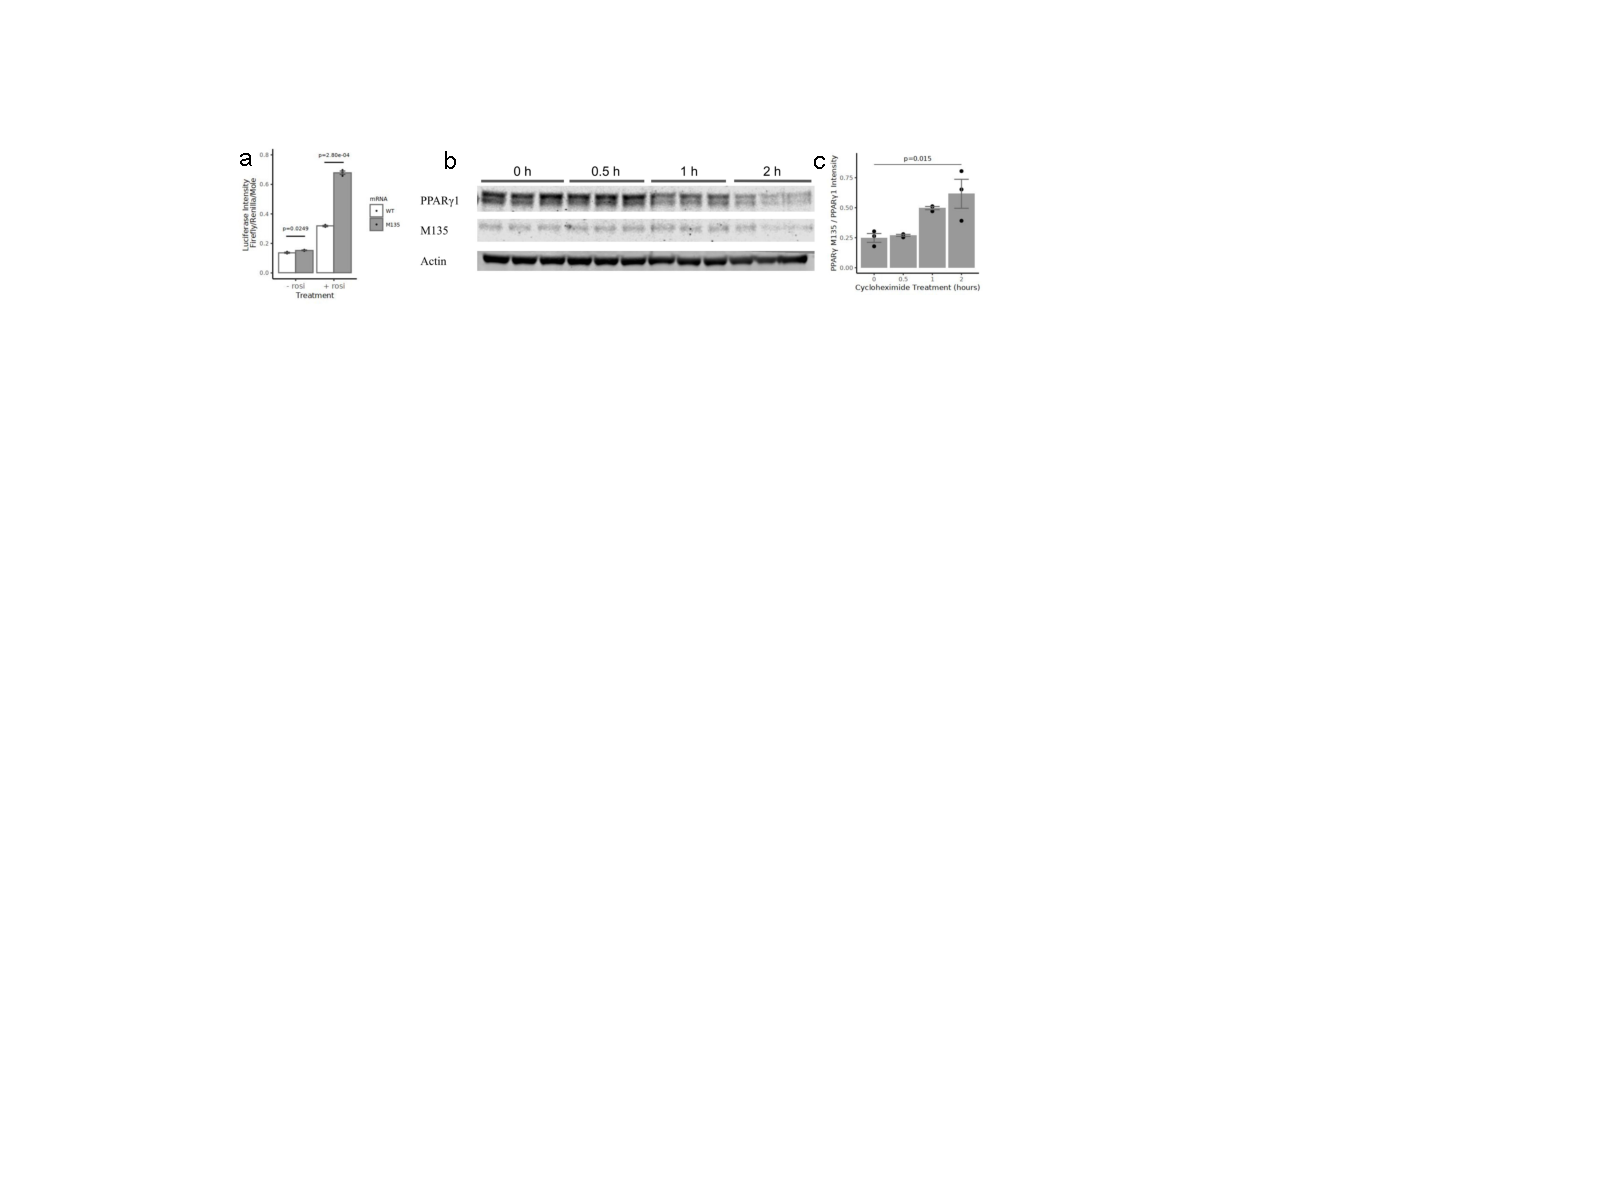
\includegraphics[width=\textwidth]{1_figures-and-files/FigS2.pdf}
    \caption[PPAR$\gamma$ M135 responds more strongly to ligands and degrades more slowly than PPAR$\gamma$1.]{\textbf{PPAR$\gamma$ M135 responds more strongly to ligands and degrades more slowly than PPAR$\gamma$1.} a. PPRE-driven luciferase promoter activity, normalized to Renilla and by mRNA moles, with 0 and 0.5 uM rosiglitazone treatments. PPAR$\gamma$ M135 activates transcription more strongly than WT PPAR$\gamma$ at baseline (n=3 each, t-test) and even more potently when stimulated with rosiglitazone (n=3 each, t-test). b. Western blot for the C-terminus of PPAR$\gamma$ in heterozygous Ex1-sgRNA THP-1 cells, which endogenously express both PPAR$\gamma$1 and PPAR$\gamma$ M135, after a 0-2 hour treatment with 5 uM cycloheximide (n=3). Actin serves as the loading control. c. Mean and sem of PPAR$\gamma$ M135/PPAR$\gamma$1 measured from b. PPAR$\gamma$ M135/PPAR$\gamma$1 increases over time after protein synthesis arrest, indicating slower degradation of PPAR$\gamma$ M135. ANOVA with Tukey post hoc test shows a significant difference between 0 and 2 hour time points.
    }
\end{figure}

\clearpage
\begin{figure}[h]
    \centering
    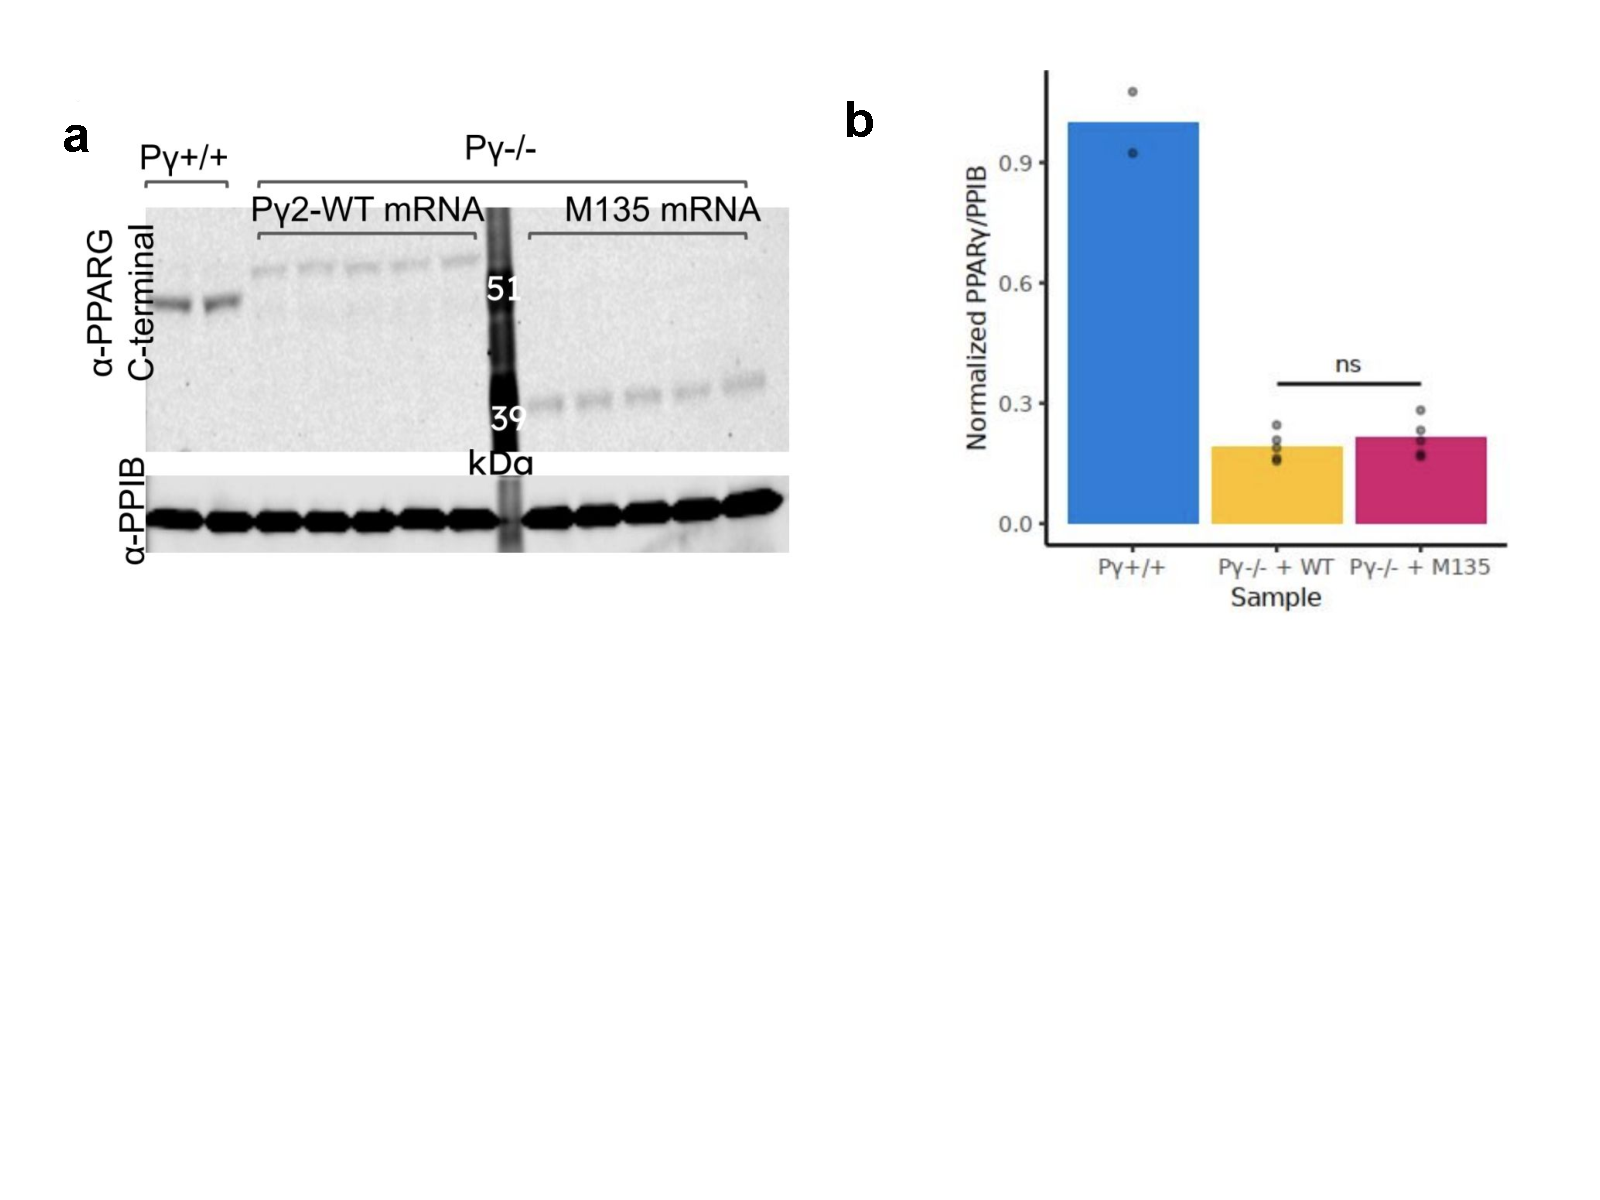
\includegraphics[width=\textwidth]{1_figures-and-files/FigS3.pdf}
    \caption[PPAR$\gamma$ protein abundance in rescue experiments.]{\textbf{PPAR$\gamma$ protein abundance in rescue experiments.} a. Western blot for the C-terminus of PPAR$\gamma$ with protein lysates from wild-type THP-1s (P$\gamma$+/+), PPAR$\gamma$ null THP-1s (P$\gamma$-/-) electroporated with PPAR$\gamma$2 wild-type (P$\gamma$2-WT) mRNA, and P$\gamma$-/- THP-1s electroporated with M135 mRNA. 8 $\mu$g WT mRNA and 2 $\mu$g M135 mRNA were electroporated to obtain similar protein expression. b. Normalized relative abundance of PPAR$\gamma$ protein in P$\gamma$+/+ (WT) THP-1, P$\gamma$-/- THP-1 electroporated with WT mRNA, and P$\gamma$-/- THP-1 electroporated with M135 mRNA. The ratio of PPAR$\gamma$ to the loading control of cyclophilin B (PPIB) was normalized to the mean of the P$\gamma$+/+ ratios, and data is presented as the mean with the data points. Statistical significance for the difference between P$\gamma$-/- + WT and P$\gamma$-/- + M135 was assessed by a two sample t-test, and the threshold used for significance was p=0.05.
    }
\end{figure}

\clearpage
\begin{table}[t]
    \centering
    \caption[Gene ontology pathway names for Figure 1.4.]{\textbf{Gene ontology pathway names for Figure 1.4.} GO IDs and pathways for the 28 pathways identified by the M135-specific DEGs.}
    \begin{tabular}{|c|m{13cm}|}
    \hline
        GO ID & GO Pathway Name \\ 
        \hline
        GO:0071674 & GOBP\_MONONUCLEAR\_CELL\_MIGRATION \\ 
        \hline
        GO:0009615 & GOBP\_RESPONSE\_TO\_VIRUS \\ \hline
        GO:0002252 & GOBP\_IMMUNE\_EFFECTOR\_PROCESS \\ \hline
        GO:0002684 & GOBP\_POSITIVE\_REGULATION\_OF\_IMMUNE\_SYSTEM\_PROCESS \\ \hline
        GO:0019079 & GOBP\_VIRAL\_GENOME\_REPLICATION \\ \hline
        GO:0006954 & GOBP\_INFLAMMATORY\_RESPONSE \\ \hline
        GO:0002711 & GOBP\_POSITIVE\_REGULATION\_OF\_T\_CELL\_MEDIATED\_IMMUNITY \\ \hline
        GO:0042330 & GOBP\_TAXIS \\ \hline
        GO:0002521 & GOBP\_LEUKOCYTE\_DIFFERENTIATION \\ \hline
        GO:0008284 & GOBP\_POSITIVE\_REGULATION\_OF\_CELL\_\newline POPULATION\_PROLIFERATION \\ \hline
        GO:0010628 & GOBP\_POSITIVE\_REGULATION\_OF\_GENE\_EXPRESSION \\ \hline
        GO:0003013 & GOBP\_CIRCULATORY\_SYSTEM\_PROCESS \\ \hline
        GO:0048878 & GOBP\_CHEMICAL\_HOMEOSTASIS \\ \hline
        GO:0051338 & GOBP\_REGULATION\_OF\_TRANSFERASE\_ACTIVITY \\ \hline
        GO:0051050 & GOBP\_POSITIVE\_REGULATION\_OF\_TRANSPORT \\ \hline
        GO:0048732 & GOBP\_GLAND\_DEVELOPMENT \\ \hline
        GO:0051301 & GOBP\_CELL\_DIVISION \\ \hline
        GO:0051130 & GOBP\_POSITIVE\_REGULATION\_OF\_CELLULAR\_\newline COMPONENT\_ORGANIZATION \\ \hline
        GO:1903047 & GOBP\_MITOTIC\_CELL\_CYCLE\_PROCESS \\ \hline
        GO:1901135 & GOBP\_CARBOHYDRATE\_DERIVATIVE\_METABOLIC\_PROCESS \\ \hline
        GO:0043254 & GOBP\_REGULATION\_OF\_PROTEIN\_CONTAINING\_\newline COMPLEX\_ASSEMBLY \\ \hline
        GO:0033865 & GOBP\_NUCLEOSIDE\_BISPHOSPHATE\_METABOLIC\_PROCESS \\ \hline
        GO:0046039 & GOBP\_GTP\_METABOLIC\_PROCESS \\ \hline
        GO:0043604 & GOBP\_AMIDE\_BIOSYNTHETIC\_PROCESS \\ \hline
        GO:0042274 & GOBP\_RIBOSOMAL\_SMALL\_SUBUNIT\_BIOGENESIS \\ \hline
        GO:0042255 & GOBP\_RIBOSOME\_ASSEMBLY \\ \hline
        GO:0042254 & GOBP\_RIBOSOME\_BIOGENESIS \\ \hline
        GO:0002181 & GOBP\_CYTOPLASMIC\_TRANSLATION \\ \hline
    \end{tabular}
\end{table}
\chapter{Supplemental Material for Chapter \ref{chap:chapter 2}}

Additional supplemental material can be found in the published location at \url{https://doi.org/10.2337/db24-0497}. 

\begin{table}[ht]
    \centering
    \caption[Human variants in \texorpdfstring{\(PPARG\)}{PPARG} upstream of M135.]{\textbf{Human variants in \texorpdfstring{\(PPARG\)}{PPARG} upstream of M135.} Each variant encodes a frameshift (fs) that results in a termination (Ter) or a stop codon (*), and the protein consequence is relative to ENSP00000287820.6. The first variant, p.Thr41ProfsTer12, encodes a stop codon at amino acid 52 on Exon 1. The second variant, p.Ile45SerfsTer8, encodes a stop codon at amino acid 52. The third variant, p.Lys63GlnfsTer7, encodes a stop codon at amino acid 69. The fourth variant, p.Ser74TyrfsTer24, results in a stop codon at amino acid 97. The fifth variant, p.Tyr78Ter, encodes a stop codon at amino acid 78. The sixth variant, p.Phe65SerfsTer33, encodes a stop codon at amino acid 97. The seventh variant, p.Gln121*, encodes a stop codon at amino acid 121. All of these occur upstream of p.M135.
  }
    \begin{tabular}{|c|c|m{4.2cm}|m{2cm}|}
    \hline
        Variant ID (hg38) & Protein Consequence & Database & Sample Size \newline (n) \\ \hline
        3-12379738-GC-G & p.Thr41ProfsTer12 & All of Us & 245400 \\ \hline
        3-12379750-TG-T & p.Ile45SerfsTer8 & Regeneron Genetics Center (RGC) Million Exome & 983578 \\ \hline
        3-12379805-A-AT & p.Lys63GlnfsTer7 & 1000G & 2548 \\ \hline
        3-12379837-C-CATTT & p.Ser74TyrfsTer24 & All of Us & 245400 \\ \hline
        3-12379855-C-G & p.Tyr78Ter & RGC Million Exome & 983578 \\ \hline
        3-12379813-CT-C & p.Phe65SerfsTer33 & RGC Million Exome & 983578 \\ \hline
        3-12381372-C-T & p.Gln121* & Framingham Heart Study (FHS) & 1637 \\ \hline
    \end{tabular}
\end{table}


\begin{figure}[ht]
    \centering
    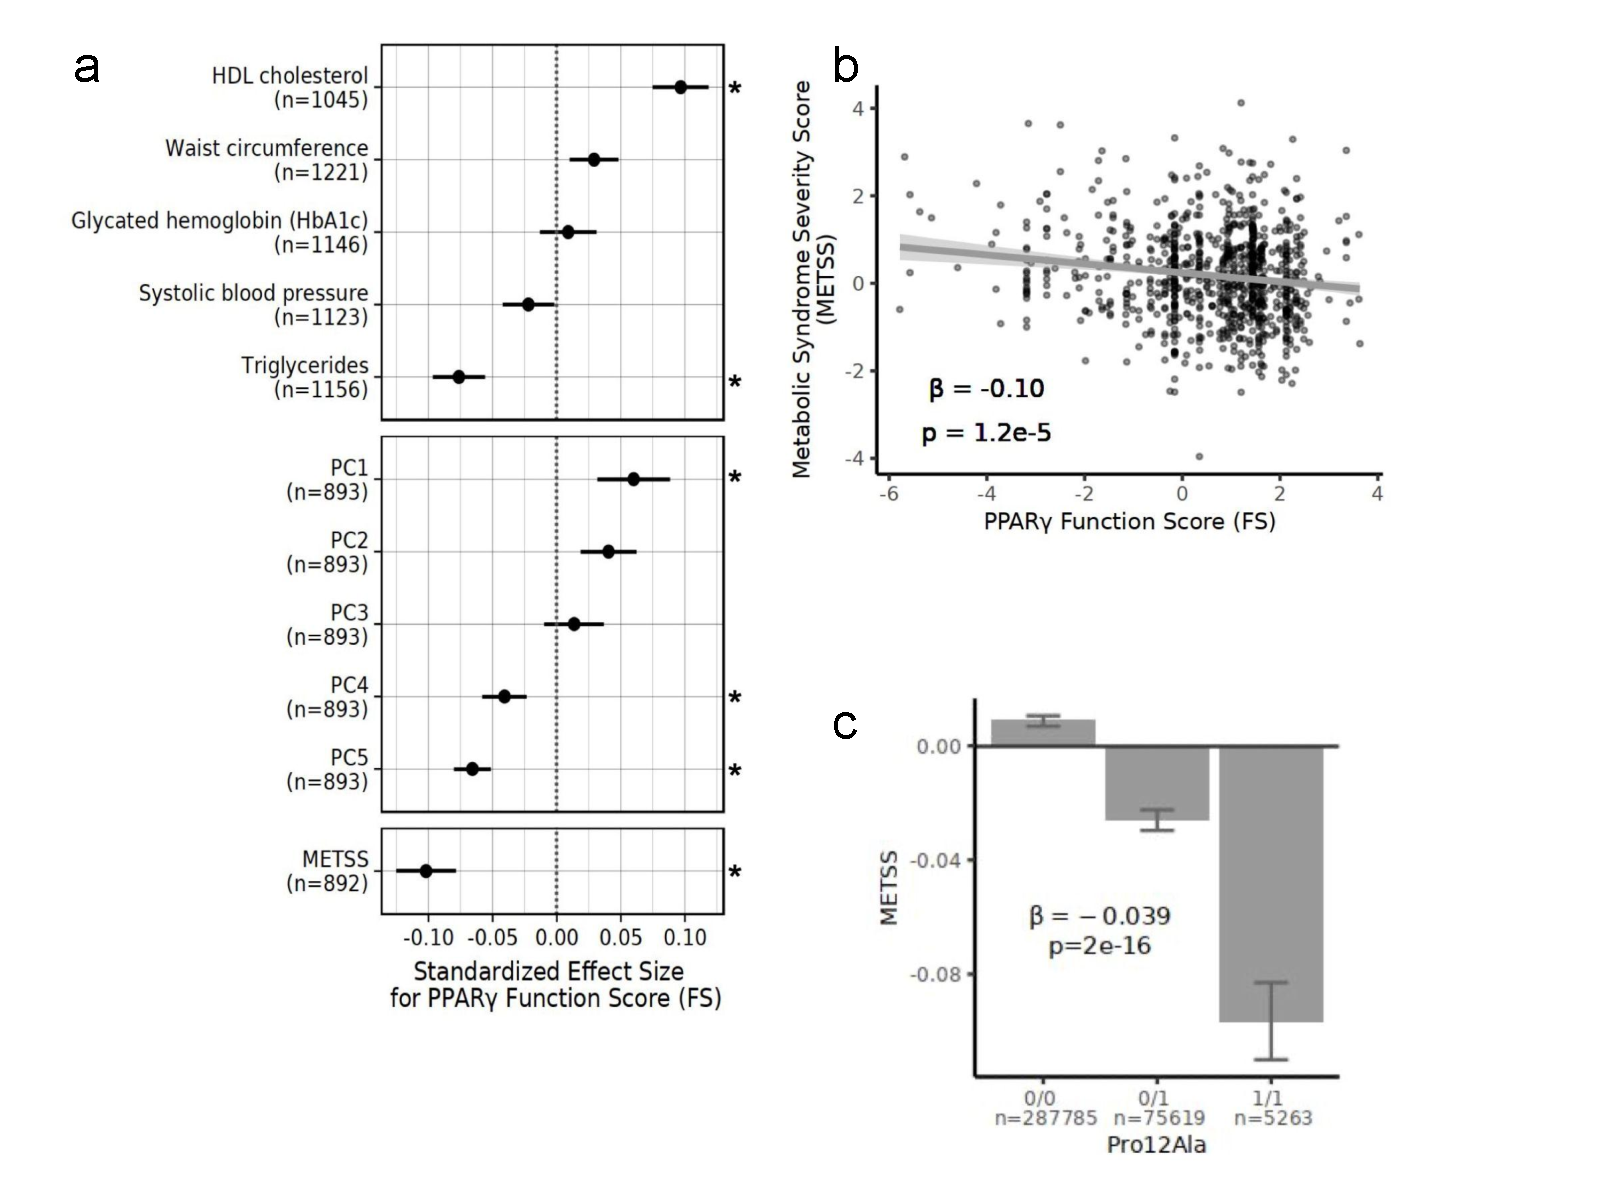
\includegraphics[width=\textwidth]{2_figures-and-files/FigS1.pdf}
    \caption[Aggregation of clinical phenotypes into a metabolic syndrome severity score (METSS).]{\textbf{Aggregation of clinical phenotypes into a metabolic syndrome severity score (METSS).} a. A metabolic syndrome severity score (METSS) was computed from five clinical phenotypes: serum HDL cholesterol, waist circumference, serum triglycerides, systolic blood pressure, and glycated hemoglobin (HbA1c). Regression coefficients for each phenotype against PPAR$\gamma$ function score (FS) are plotted with covariate adjustments for age, age2, sex, and 10 genetic principal components. Only serum triglycerides and HDL cholesterol show significant regression slopes. Analogous regression analysis was performed and plotted for principal components (PCs) derived from dimensionality reduction (i.e. PCA) performed on the five clinical phenotypes. PC1, PC4 and PC5 had significant effect sizes when regressed against the PPAR$\gamma$ FS. Standardized effect size (dot) and standard error (lines) are shown for each value; the sample size is the number of individuals with each phenotype/PC and the PPAR$\gamma$ FS, and significance was determined by p $<$ 0.05. Only 892 individuals were carriers of rare, protein-coding \(PPARG\) variants with PPAR$\gamma$ FS and had computable METSS. b. In carriers of \(PPARG\) missense variants with METSS (n=892), the metabolic syndrome severity score decreases with increasing PPAR$\gamma$ function (linear regression, effect size = -0.10, p=1.2e-5). c. Mean and sem of METSS by Pro12Ala genotype. METSS decreases with increasing alleles of the alternate, as modeled by METSS ~ number of alternate alleles, which has effect size of -0.039 and p-value=2e-16.
    }
\end{figure}


%%%%%%%%%%%%%%%%%%%%%%%%%%%%%%%%%%%%%%%%%%%%%%%%%%%%%%%%%%%%%%%%%%%%%%%%%%%%%%%%
% End of the Dissertation
%%%%%%%%%%%%%%%%%%%%%%%%%%%%%%%%%%%%%%%%%%%%%%%%%%%%%%%%%%%%%%%%%%%%%%%%%%%%%%%%
%\backmatter{}
%\bibliographystyle{unsrtnat} 
%\bibliography{bibliography}

\end{document}
